\newcommand\thesistypedebug{}
\newcommand\thesistitle{Masterthesis}
%\newcommand\thesissubtitle{Orderbook Agent}
\newcommand\thesisdate{July 31, 2017}

% -- Vektor fett darstellen -----------------
% \let\oldvec\vec
% \def\vec#1{{\boldsymbol{#1}}} %Fetter Vektor
% \newcommand{\ve}{\vec} %
% -------------------------------------------

\newcommand{\itemmath}[1]{$\bm{\mathsf{#1}}$}
\newcommand{\captionmath}[1]{$\protect\captionmathfont{#1}$}
  \newcommand{\captionmathfonttoc}[1]{\mathsf{#1}}
  \newcommand{\captionmathfonttext}[1]{\bm{\mathsf{#1}}}
  \let\captionmathfont=\captionmathfonttext
\newcommand{\sectionmath}[1]{$\protect\sectionmathfont{#1}$}
  \newcommand{\sectionmathfonttoc}[1]{#1}
  \newcommand{\sectionmathfonttext}[1]{\mathsf{#1}}
  \let\sectionmathfont=\sectionmathfonttext

%% from package braket
{\catcode`\|=\active
  \xdef\Concat{\protect\expandafter\noexpand\csname Concat \endcsname}
  \expandafter\gdef\csname Concat \endcsname#1{\begingroup
     \ifx\SavedDoubleVert\relax
       \let\SavedDoubleVert\|\let\|\BraDoubleVert
     \fi
     \mathcode`\|32768\let|\BraVert
     \left[{#1}\right]\endgroup}
}

\newcommand{\mathup}[1]{\mathrm{#1}}

\newcommand\eref[1]{\tag*{\ref{#1}}} % Formel erscheint erneut und soll gleiche Formelnummer wie beim ersten Auftreten erhalten

\newcommand\const{\mathrm{const}}
\newcommand\rp{^{-1}}
\newcommand\rps{^{-2}}
\newcommand\rpc{^{-3}}

\newcommand\transpose{^T} %{^\top}
\newcommand\rptranspose{^{-T}} %^{^{-\top}}
\newcommand\pseudoinverse{^{+}}

\newcommand\define{:=} % :=, \ensuremath{\mathrel{\stackrel{\mathrm{def}}{=}}}
\newcommand\ldefine{=:}
\newcommand{\setsep}{\, | \,}
%\newcommand\set[1]{\left{#1\right}}
%\newcommand\set*[2]{\left{ #1 \setsep #2 \right}}
%\newcommand{\set}[2][]{%
%    \ifthenelse{\equal{#1}{}}{\left\{ #2 \right\}}{\left\{ #1 \setsep #2 \right\}}%
%  }

\newcommand{\norm}[1]{\left\Vert #1 \right\Vert_2}
\newcommand{\floor}[1]{\left\lfloor #1 \right\rfloor}
\newcommand{\ceil}[1]{\left\lceil #1 \right\rceil}

%\newcommand{\vecval}[1]{\mathbf{#1}}
\newcommand{\vecval}[1]{{\color{MathsVectorColor}\bm{#1}}}
\newcommand{\matval}[1]{{\color{MathsMatrixColor}#1}}
  %\newcommand{\vecval}[1]{\bm{#1}}
  %\newcommand{\matval}[1]{#1}

\newcommand{\sspace}{\quad}
\newcommand{\wspace}{\qquad}

\newcommand{\sand}{\sspace\text{and}\sspace}
\newcommand{\wand}{\wspace\text{and}\wspace}
\newcommand{\for}{\text{for }}

\newcommand{\R}{\mathbb{R}}
\newcommand{\N}{\mathbb{N}}

\newcommand{\unitvec}[2]{{\vecval{u}_{#1}^{(#2)}}}
\newcommand{\identitymat}[1]{\matval{\mathup{I}}_{#1,#1}}
\newcommand{\permutemat}{\matval{\Pi}}
\newcommand{\zerovec}[1]{\vecval{0}_{#1}}
\newcommand{\zeromat}[2]{\matval{0}_{#1,#2}}

\newcommand{\eqnannotate}[1]{\tag*{\color{AnnotationColor} #1}}
\newcommand{\eqnannotatefrom}[2][]{\eqnannotate{#1 from \Cref{#2}}}
\newcommand{\eqnannotatecf}[1]{\eqnannotate{\cf (\explicitref{#1})}}
\newcommand{\equalref}[1]{\,\stackrel{\text{\footnotesize(\explicitref{#1})}}{=}\,}

\newcommand{\fulfill}{\stackrel{!}{=}}
\newcommand{\inlineortho}{\bot}
\newcommand{\ortho}{\,\, \inlineortho \,\,}
\newcommand{\iszero}[1]{\underbrace{#1}_{=0}}

\newcommand{\vecsize}[1]{\in\R^{#1}}
\newcommand{\matsize}[2]{\in\R^{#1 \times #2}}

\newcommand{\Tsstep}[1]{\matval{\overline{#1}}}
\newcommand{\sstep}[1]{\matval{\overline{#1}}}
\newcommand{\Sstep}[1]{\matval{\ddot{#1}}}
\newcommand{\dual}[1]{\matval{\hat{#1}}}
\newcommand{\dualvec}[1]{\hat{#1}}
\newcommand{\append}[1]{\underline{#1}}

%\newcommand{\ATpower}[1]{{\left( \matval{A}\transpose \right)}^{#1}}
\newcommand{\ATpower}[1]{{( \matval{A}\transpose )}^{#1}}
\newcommand{\bracketT}[1]{{\left( #1 \right)}\transpose}

\newcommand{\abs}[1]{\left\lvert #1 \right\rvert}
\newcommand{\linearspan}[1]{\mathrm{span}\left( #1 \right)}
\newcommand{\conj}[1]{\overline{#1}}

\newcommand{\concatmat}[1]{\Concat{#1}}
\newcommand{\concatvec}[1]{\left[#1\right]}
\newcommand{\concatmatsep}{\, | \,}
%\newcommand{\lincomb}[1]{\left\langle #1 \right\rangle}
\newcommand{\lincomb}[1]{\linearspan{#1}}
%\newcommand{\vecprod}[2]{\left( #1, #2 \right)}
\newcommand{\vecprod}[2]{\left\langle #1, #2 \right\rangle}

%\newcommand{\sign}[1]{\mathrm{sign}\left( #1 \right)}
%\newcommand{\ssign}{\mathrm{sign}}
\newcommand{\diag}{\operatorname{diag}}
%\renewcommand\Re[1][]{\mathrm{Re}\,#1}
%\renewcommand\Im[1][]{\mathrm{Im}\,#1}

\newcommand{\vvector}[2]{\left[\begin{array}{c} #1 \\ #2 \end{array} \right]}
\newcommand{\vvvector}[3]{\left[\begin{array}{c} #1 \\ #2 \\ #3 \end{array} \right]}

\newcommand{\intervaloo}[2]{\left(#1,#2\right)}
\newcommand{\intervaloc}[2]{\left(#1,#2\right]}
\newcommand{\intervalco}[2]{\left[#1,#2\right)}
\newcommand{\intervalcc}[2]{\left[#1,#2\right]}

\newenvironment{mmatrix}{\begin{bmatrix}}{\end{bmatrix}}

\newcommand{\Oh}[1]{\mathrm{O}\left(#1\right)}

\newcommand{\e}[1]{\mathup{e}^{#1}}

\newcommand{\dd}{\mathop{}\!\mathrm{d}}
\newcommand{\Laplace}{\mathrm{\Delta}}

\newcommand\op[1]{{\hat{\mathrm{#1}}}}  % Operator

\newcommand\imaginary{\mathup{i}}

% use together with long limits in \sum, \prod, etc
% from mathmode, p. 63
  \def\clap#1{\hbox to 0pt{\hss#1\hss}}
  \def\mathclap{\mathpalette\mathclapinternal}
  \def\mathclapinternal#1#2{%
    \clap{$\mathsurround=0pt#1{#2}$}
  }
	
	
\newcommand{\argmax}{\operatornamewithlimits{arg \, max}}


\newcommand\ie{i.\,e.\xspace}
\newcommand\eg{e.\,g.\xspace}
\newcommand\Eg{E.\,g.\xspace}
\newcommand\NB{N.\,B.\xspace}
\newcommand\BSc{B.\,Sc.\xspace}
\newcommand\MSc{M.\,Sc.\xspace}
\newcommand\PhD{Ph.\,D.\xspace}
\newcommand\etc{etc.\xspace}
\newcommand\cf{cf.\xspace}
\newcommand\Cf{Cf.\xspace}
\newcommand\etal{et\,al.\xspace}
\newcommand\page[1]{p.\,#1}
\newcommand\pages[1]{pp.\,#1}

\newcommand\zB{z.\,B.\xspace}
\newcommand\proz{\,\%\xspace}

\newcommand\thesis{thesis\xspace}
%\newcommand\person[1]{#1} % f�r Personennamen
%\newcommand\software[1]{#1} % f�r Softwarenamen
%\newcommand\name[1]{\textsc{#1}} % f�r Personennamen
\newcommand\software[1]{\textsc{#1}} % f�r Softwarenamen

\newcommand\Index[1]{#1\index{#1}} % f�r Eintr�ge, die im Text als auch im Index erscheinen sollen

\newcommand\cell[1]{\textcolor{gray}{#1}} % f�r Excel-Zellen
\newcommand\stress[1]{\emph{\Index{#1}}} % Hervorhebung von Schl�sselw�rtern in Definitionen
%%\newcolumntype{Q}{>{$}r<{$}}
%\newcolumntype{C}{>{$}c<{$}}
%\newcolumntype{J}{>{$}l<{$}}

%\newcolumntype{.}[1]{D{.}{,}{#1}}
%\newcolumntype{,}[1]{D{,}{,}{#1}}

%% Kommandos fuer Tabellen. Entnommen aus The LateX Companion, tabsatz.ps und diversen Dokus:

%%% ---| Farben fuer Tabellen |-------------------
\IfPackageLoaded{xcolor}{
   \colorlet{tablesubheadcolor}{gray!30}
   \colorlet{tableheadcolor}{gray!25}
   \colorlet{tableblackheadcolor}{black!100}
   \colorlet{tablerowcolor}{gray!10.0}
}
%%% ---------------------------------------------


%%% -| Neue Spaltendefinitionen 'columntypes' |--
%
% Belegte Spaltentypen:
% l - links
% c - zentriert
% r - rechts
% p,m,b  - oben, mittig, unten
% X - tabularx Auto-Spalte

% um Tabellenspalten mit Flattersatz zu setzen, muss \\ vor
% (z.B.) \raggedright geschuetzt werden:
\newcommand{\PreserveBackslash}[1]{\let\temp=\\#1\let\\=\temp}


% Spalten mit Flattersatz und definierte Breite:
% m{} -> mittig
% p{} -> oben
% b{} -> unten
%
% Linksbuendig:
\newcolumntype{v}[1]{>{\PreserveBackslash\RaggedRight\hspace{0pt}}p{#1}}
\newcolumntype{M}[1]{>{\PreserveBackslash\RaggedRight\hspace{0pt}}m{#1}}
% % Rechtsbuendig :
% \newcolumntype{R}[1]{>{\PreserveBackslash\RaggedLeft\hspace{0pt}}m{#1}}
% \newcolumntype{S}[1]{>{\PreserveBackslash\RaggedLeft\hspace{0pt}}p{#1}}
% % Zentriert :
% \newcolumntype{Z}[1]{>{\PreserveBackslash\Centering\hspace{0pt}}m{#1}}
% \newcolumntype{A}[1]{>{\PreserveBackslash\Centering\hspace{0pt}}p{#1}}

\newcolumntype{Y}{>{\PreserveBackslash\RaggedLeft\hspace{0pt}}X}
%%% Spalten fuer Mathematik
%
% serifenlose Matheschrift
%\newcolumntype{s}[1]{%
%  >{\DC@{.}{,}{#1}\mathsf\bgroup}l%
%  <{\egroup\DV@end}%
%}

% Tabellenspaltentyp fuer den Kopf: (Farbe + Ausrichtung)
\newcolumntype{H}[1]{>{\columncolor{tableheadcolor}}l}

% aequivalent aus typokurz (fett+grau+links)
% \newcolumntype{H}{>{\fontseries{b}\selectfont%
%     \columncolor[gray]{.8}[6pt][0pt]}l}
%%% --------------------------------------------


%%% ---|Listen in Tabellen |--------------------
\newcommand{\removeindentation}{%
  \leftmargini=\labelsep%
  \advance\leftmargini by \labelsep%
}
%
\makeatletter
\newcommand\tableitemize{
  \@minipagetrue%
  \removeindentation
}
\makeatother
%%% --------------------------------------------

%%% ---|Layout der Tabellen |-------------------

% Neue Umgebung fuer Tabellen:

\newenvironment{Tabelle}[2][c]{%
  \tablestylecommon
  \begin{longtable}[#1]{#2}
  }
  {\end{longtable}%
  \tablerestoresettings
}


% Groesse der Schrift in Tabellen
\newcommand{\tablefontsize}{ \footnotesize}
\newcommand{\tableheadfontsize}{\footnotesize}

% Layout der Tabelle: Ausrichtung, Schrift, Zeilenabstand
\newcommand\tablestylecommon{%
  \renewcommand{\arraystretch}{1.4} % Groessere Abstaende zwischen Zeilen
  \normalfont\normalsize            %
  \sffamily\tablefontsize           % Serifenlose und kleine Schrift
  \centering%                       % Tabelle zentrieren
}

\newcommand{\tablestyle}{
  \tablestylecommon
  %\tablealtcolored
}

% Ruecksetzten der Aenderungen
\newcommand\tablerestoresettings{%
  \renewcommand{\arraystretch}{1}% Abstaende wieder zuruecksetzen
  \normalsize\rmfamily % Schrift wieder zuruecksetzen
}

% Tabellenkopf: Serifenlos+fett+schraeg+Schriftfarbe
\newcommand\tablehead{%
  \tableheadfontsize%
  \sffamily\bfseries%
  %\slshape
  %\color{white}
}

\newcommand\tablesubheadfont{%
  \tableheadfontsize%
  \sffamily\bfseries%
  \slshape
  %\color{white}
}


\newcommand\tableheadcolor{%
  %\rowcolor{tablesubheadcolor}
  %\rowcolor{tableblackheadcolor}
  \rowcolor{tableheadcolor}%
}

\newcommand\tablesubheadcolor{%
  \rowcolor{tablesubheadcolor}
  %\rowcolor{tableblackheadcolor}
}


\newcommand{\tableend}{\arrayrulecolor{black}\hline}

% Tabellenkopf (1=Spaltentyp, 2=Text)
% \newcommand{\tablehead}[2]{
%   \multicolumn{1}{#1@{}}{%
%     \raisebox{.1mm}{% Ausrichtung der Beschriftung
%       #2%
%     }\rule{0pt}{4mm}}% unsichtbare Linie, die die Kopfzeile hoeher macht
% }


\newcommand{\tablesubhead}[2]{%
  \multicolumn{#1}{>{\columncolor{tablesubheadcolor}}l}{\tablesubheadfont #2}%
}

% Tabellenbody (=Inhalt)
\newcommand\tablebody{%
\tablefontsize\sffamily\upshape%
}

\newcommand\tableheadshaded{%
  \rowcolor{tableheadcolor}%
}
\newcommand\tablealtcolored{%
  \rowcolors{1}{tablerowcolor}{white!100}%
}
%%% --------------------------------------------

\newlength{\mylen}
\newlength{\adjusthspace}

\newenvironment{tabularc}[2]
{%
  \setlength\mylen{#2/(#1)-\tabcolsep*2-\arrayrulewidth*(#1+1)/(#1)}%
  %\setlength{\adjusthspace}{((#2-1)/2)*\linewidth}
  %\par\noindent
  %\hspace*{-\the\adjusthspace}
  \begin{tabular}%{#2}%
    {*{#1}{v{\the\mylen}}}%
}
{\end{tabular}\par}

 
%% Document class: Koma Script
\documentclass[%
   %draft,     % Entwurfsstadium
   final,      % fertiges Dokument
   % --- Paper Settings ---
   paper=a4,% [Todo: add alternatives]
   paper=portrait, % landscape
   pagesize=auto, % driver
	 abstracton,
   % --- Koma Script Version ---
   version=last, %
 ]{scrartcl} % Classes: scrartcl, scrreprt, scrbook

%%% === Headings ==============================================================
\KOMAoptions{%
   %%%% headings
   %headings=small,  % Small Font Size, thin spacing above and below
   % headings=normal, % Medium Font Size, medium spacing above and below
   %headings=big, % Big Font Size, large spacing above and below
   %
   %headings=noappendixprefix, % chapter in appendix as in body text
   %headings=nochapterprefix,  % no prefix at chapters
   % headings=appendixprefix,   % inverse of 'noappendixprefix'
   % headings=chapterprefix,    % inverse of 'nochapterprefix'
   %headings=openany,   % Chapters start at any side
   % headings=openleft,  % Chapters start at left side
   % headings=openright, % Chapters start at right side      
   %%% Add/Dont/Auto Dot behind section numbers 
   %%% (see DUDEN as reference)
   % numbers=autoenddot
   % numbers=enddot %<--Header punkt nach zahl
   numbers=noenddot,
   % secnumdepth=3 % depth of sections numbering (???)
}%

\setcounter{secnumdepth}{3}

%%% === Page Layout ===========================================================
\KOMAoptions{% (most options are for package typearea)
   % twoside=false, % two side layout (alternating margins, standard in books)
   % twoside=false, % single side layout 
   twoside=semi,  % two side layout (non alternating margins!)
   %
   twocolumn=false, % (true)
   %
   headinclude=true,%
   footinclude=false,%
   mpinclude=false,%      
   %
   headlines=2.1,%
   % headheight=2em,%
   headsepline=true,%
   footsepline=false,%
   cleardoublepage=empty %plain, headings
}%

%%% === Paragraph Separation ==================================================
\KOMAoptions{%
  % parskip=relative, % change indentation according to fontsize (recommanded)
   parskip=absolute, % do not change indentation according to fontsize
   parskip=false,    % indentation of 1em
   % parskip=true   % parksip of 1 line - with free space in last line of 1em
   % parskip=full-  % parksip of 1 line - no adjustment
   % parskip=full+  % parksip of 1 line - with free space in last line of 1/4
   % parskip=full*  % parksip of 1 line - with free space in last line of 1/3
   % parskip=half   % parksip of 1/2 line - with free space in last line of 1em
   % parskip=half-  % parksip of 1/2 line - no adjustment
   % parskip=half+  % parksip of 1/2 line - with free space in last line of 1/3
   % parskip=half*  % parksip of 1/2 line - with free space in last line of 1em
}%

%%% === Table of Contents =====================================================
\setcounter{tocdepth}{3} % Depth of TOC Display
\KOMAoptions{%
   %%% Setting of 'Style' and 'Content' of TOC
   % toc=left, %
   toc=indented,%
   %
   toc=bib,
   % toc=nobib,
   % toc=bibnumbered,
   %
   % toc=index,%
   toc=noindex,
   %
    toc=listof,
   %toc=nolistof
   % toc=listofnumbered,
   %    
}%  
%%% === Lists of figures, tables etc. =========================================
\KOMAoptions{%
   %%% Setting of 'Style' and 'Content' of Lists 
   %%% (figures, tables etc)
  % --- General List Style ---
   %listof=left, % tabular styles
   %listof=indented, % hierarchical style
   % --- chapter highlighting ---
   % listof=chapterentry, % ??? Chapter starts are marked in figure/table
   % listof=chaptergapline, % New chapter starts are marked by a gap 
                        % of a single line
   % listof=chaptergapsmall, % New chapter starts are marked by a gap 
                      % of a smallsingle line
   %listof=nochaptergap, % No Gap between chapters
   %
   % listof=leveldown, % lists are moved one level down ???
   % --- Appearance of Lists in TOC
   %listof=notoc, % Lists are not part of the TOC
   % listof=totoc % add Lists to TOC without number
    listof=totocnumbered, % add Lists to TOC with number
}%  

%%% === Bibliography ==========================================================
%% Setting of 'Style' and 'Content' of Bibliography
\KOMAoptions{%
   % bibliography=oldstyle,%
   bibliography=openstyle,%
   % bibliography=nottotoc, % Bibliography is not part of the TOC
    bibliography=totocnumbered, % add Bibliography to TOC with number
   %bibliography=totoc % add Bibliography to TOC without number
}%

%%% === Index =================================================================
%% Setting of 'Style' and 'Content' of Index in TOC
\KOMAoptions{%
   index=nottotoc % index is not part of the TOC
  % index=totoc, % add index to TOC without number
}%
 
%%% === Titlepage =============================================================
\KOMAoptions{%
   titlepage=true %
   %titlepage=false %
}%

%%% === Page / Font size ======================================================
\KOMAoptions{%
   % --- Base Font Size ---
   fontsize=11pt,%
	%\linespread{1.25}
 %  DIV=9,% Default: 8 for 10pt, 10 for 11pt, 11 for 12pt
}%

%%% === Miscellaneous =========================================================
\KOMAoptions{%   
   footnotes=multiple% nomultiple
   %open=any,%
   %open=left,%
   %open=right,%
   %chapterprefix=false,%
   %appendixprefix=false,%
   %chapteratlists=10pt,% entry
}%


\usepackage{scrhack}
% Encoding der Dateien (sonst funktionieren Umlaute nicht)
% Fuer Linux -> utf8
% Fuer Windows, alte Linux Distributionen -> latin1
  
% Empfohlen latin1, da einige Pakete mit utf8 Zeichen nicht
% funktionieren, z.B: listings, soul. 
\usepackage[latin1]{inputenc}
%\usepackage[ansinew]{inputenc}
%\usepackage[utf8]{inputenc}
%\usepackage{ucs}
%\usepackage[utf8x]{inputenc}
%%% Packages for LaTeX - programming
%
% Define commands that don't eat spaces.
\usepackage{xspace}
% IfThenElse
\usepackage{ifthen}

%%% Doc: http://www.bakoma-tex.com/doc/latex/oberdiek/ifdraft.pdf
%% Usage: \iffdraft{draft-Modus}{final-Modus}
\usepackage{ifdraft}

%%% Doc: ftp://tug.ctan.org/pub/tex-archive/macros/latex/contrib/oberdiek/ifpdf.sty
% command for testing for pdf-creation
\usepackage{ifpdf} %\ifpdf \else \fi
 
%%% Internal Commands: ----------------------------------------------
\makeatletter
%
\providecommand{\IfPackageLoaded}[2]{\@ifpackageloaded{#1}{#2}{}}
\providecommand{\IfPackageNotLoaded}[2]{\@ifpackageloaded{#1}{}{#2}}
\providecommand{\IfElsePackageLoaded}[3]{\@ifpackageloaded{#1}{#2}{#3}}
%
\newboolean{chapteravailable}%
\setboolean{chapteravailable}{false}%
 
\ifcsname chapter\endcsname
  \setboolean{chapteravailable}{true}%
\else
  \setboolean{chapteravailable}{false}%
\fi
 
 
\providecommand{\IfChapterDefined}[1]{\ifthenelse{\boolean{chapteravailable}}{#1}{}}%
\providecommand{\IfElseChapterDefined}[2]{\ifthenelse{\boolean{chapteravailable}}{#1}{#2}}%
 
\providecommand{\IfDefined}[2]{%
\ifcsname #1\endcsname
   #2 %
\else
     % do nothing
\fi
}
%
% Check for 'draft' mode - commands.
\newcommand{\IfNotDraft}[1]{\ifdraft{}{#1}}
\newcommand{\IfNotDraftElse}[2]{\ifdraft{#2}{#1}}
\newcommand{\IfDraft}[1]{\ifdraft{#1}{}}
 
% Definde frontmatter, mainmatter and backmatter if not defined
\@ifundefined{frontmatter}{%
   \newcommand{\frontmatter}{%
      %In Roemischen Buchstaben nummerieren (i, ii, iii)
      \pagenumbering{roman}
			\hypersetup{pageanchor=false}
   }
}{}
\@ifundefined{mainmatter}{%
   % scrpage2 benoetigt den folgenden switch
   % wenn \mainmatter definiert ist.
   \newif\if@mainmatter\@mainmattertrue
   \newcommand{\mainmatter}{%
      % -- Seitennummerierung auf Arabische Zahlen zuruecksetzen (1,2,3)
      \pagenumbering{arabic}%
      \hypersetup{pageanchor=true}
   }
}{}
\@ifundefined{backmatter}{%
   \newcommand{\backmatter}{
      %In Roemischen Buchstaben nummerieren (i, ii, iii)
      \pagenumbering{roman}
			\hypersetup{pageanchor=true}

			
   }
}{}
 
% Pakete speichern die spaeter geladen werden sollen
\newcommand{\LoadPackagesNow}{}
\newcommand{\LoadPackageLater}[1]{%
   \g@addto@macro{\LoadPackagesNow}{%
      \usepackage{#1}%
   }%
}
 
 
 
\makeatother
%%% ----------------------------------------------------------------
% ~~~~~~~~~~~~~~~~~~~~~~~~~~~~~~~~~~~~~~~~~~~~~~~~~~~~~~~~~~~~~~~~~~~~~~~~
% Einige Pakete muessen unbedingt vor allen anderen geladen werden
% ~~~~~~~~~~~~~~~~~~~~~~~~~~~~~~~~~~~~~~~~~~~~~~~~~~~~~~~~~~~~~~~~~~~~~~~~
 
%%% Doc: www.cs.brown.edu/system/software/latex/doc/calc.pdf
% Calculation with LaTeX
\usepackage{calc}
 
%%% Doc: ftp://tug.ctan.org/pub/tex-archive/macros/latex/required/babel/babel.pdf
% Languagesetting
\usepackage[
%  german,
%  ngerman,
  english,
%  frensh,
]{babel}

%%% Info: http://www.mail-archive.com/ctan-ann@dante.de/msg01512.html
% For adding/using translations like "Theorem/Satz" inside babel, especially for beamer
\usepackage{translator}
 
%%% Doc: ftp://tug.ctan.org/pub/tex-archive/macros/latex/contrib/xcolor/xcolor.pdf
% Farben
% Incompatible: Do not load when using pstricks !
\usepackage[
  dvipsnames,
  table % Load for using rowcolors command in tables
]{xcolor}
 
 
%%% Doc: ftp://tug.ctan.org/pub/tex-archive/macros/latex/required/graphics/grfguide.pdf
% Bilder
\usepackage[%
  %final,
  %draft % do not include images (faster)
]{graphicx}
 
%%% Doc: ftp://tug.ctan.org/pub/tex-archive/macros/latex/contrib/oberdiek/epstopdf.pdf
%% If an eps image is detected, epstopdf is automatically called to convert it to pdf format.
%% Requires: graphicx loaded
\usepackage{epstopdf}
 
 
%%% Doc: ftp://tug.ctan.org/pub/tex-archive/macros/latex/required/amslatex/math/amsldoc.pdf
% Amsmath - Mathematik Basispaket
%
% fuer pst-pdf displaymath Modus vor pst-pdf benoetigt.
\usepackage[
   centertags, % (default) center tags vertically
   %tbtags,    % 'Top-or-bottom tags': For a split equation, place equation numbers level
               % with the last (resp. first) line, if numbers are on the right (resp. left).
   sumlimits,  %(default) Place the subscripts and superscripts of summation
               % symbols above and below
   %nosumlimits, % Always place the subscripts and superscripts of summation-type
               % symbols to the side, even in displayed equations.
   intlimits,  % Like sumlimits, but for integral symbols.
   %nointlimits, % (default) Opposite of intlimits.
   namelimits, % (default) Like sumlimits, but for certain 'operator names' such as
               % det, inf, lim, max, min, that traditionally have subscripts placed underneath
               % when they occur in a displayed equation.
   %nonamelimits, % Opposite of namelimits.
   %leqno,     % Place equation numbers on the left.
   %reqno,     % Place equation numbers on the right.
   %fleqn,     % Position equations at a fixed indent from the left margin rather than
               % centered in the text column.
]{amsmath} %
% eqnarray nicht zusammen mit amsmath benutzen, siehe l2tabu.pdf f�r Hintergruende.
 
%%% Doc: http://www.ctan.org/tex-archive/macros/latex/contrib/pst-pdf/pst-pdf-DE.pdf
% Used to automatically integrate eps graphics in an pdf document using pdflatex.
% Requires ps4pdf macro !!!
% Download macro from http://www.ctan.org/tex-archive/macros/latex/contrib/pst-pdf/scripts/
%
\usepackage[%
   %active,       % Aktiviert den Extraktionsmodus (DVI-Ausgabe). Die explizite Angabe ist
                  % normalerweise unn�tig (Standard im LATEX-Modus).
   %inactive,     % Das Paket wird deaktiviert, Zu�tzlich werden die Pakete pstricks und
                  % graphicx geladen
   nopstricks,    % Das Paket pstricks wird nicht geladen.
   %draft,        % Im pdfLATEX-Modus werden aus der Containerdatei eingef�gte Grafiken nur
                  % als Rahmen dargestellt.
   %final,        % Im pdfLATEX-Modus werden aus der Containerdatei eingef�gte Grafiken
                  % vollst�ndig dargestellt (Standard).
   %tightpage,    % Die Abmessung Grafiken in der Containerdatei entsprechen denen der
                  % zugeh�rigen TEX-Boxen (Standard).
   %notightpage,  % die Grafiken in der Containerdatei nehmen
                  % mindestens die Gr��e des gesamten Blattes einnehmen.
   displaymath,   %  Es werden zus�tzlich die mathematischen Umgebungen displaymath,
                  % eqnarray und $$ extrahiert und im pdf-Modus als Grafik eingef�gt.
]{pst-pdf}
%
% Notwendiger Bugfix f�r natbib Paket bei Benutzung von pst-pdf (Version <= v1.1o)
\IfPackageLoaded{pst-pdf}{
   \providecommand\makeindex{}
   \providecommand\makeglossary{}
}{}
 
 
%% Doc: ftp://tug.ctan.org/pub/tex-archive/graphics/pstricks/README
% load before graphicx
% \usepackage{pstricks}
% \usepackage{pst-plot, pst-node, pst-coil, pst-eps}
 
% This package implements a workaround for the LaTeX bug that marginpars
% sometimes appear on the wrong margin.
% \usepackage{mparhack}
% in some case this causes an error in the index together with package pdfpages
% the reason is unkown. Therefore I recommend to use the margins of marginnote
  
%% Doc: (inside relsize.sty )
%% ftp://tug.ctan.org/pub/tex-archive/macros/latex/contrib/misc/relsize.sty
%  Set the font size relative to the current font size
\usepackage{relsize}
 
%% Doc: ftp://tug.ctan.org/pub/tex-archive/macros/latex/contrib/ms/ragged2e.pdf
% Besserer Flatternsatz (Linksbuendig, statt Blocksatz)
\usepackage{ragged2e}
% ~~~~~~~~~~~~~~~~~~~~~~~~~~~~~~~~~~~~~~~~~~~~~~~~~~~~~~~~~~~~~~~~~~~~~~~~
% Fonts Fonts Fonts
% ~~~~~~~~~~~~~~~~~~~~~~~~~~~~~~~~~~~~~~~~~~~~~~~~~~~~~~~~~~~~~~~~~~~~~~~~
 
\usepackage[T1]{fontenc} % T1 Schrift Encoding
\usepackage{textcomp}   % Zusatzliche Symbole (Text Companion font extension)
 
% Alle Schriften die hier angegeben sind sehen im PDF richtig aus.
% Die LaTeX Standardschrift ist die Latin Modern (lmodern Paket).
% If Latin Modern is not available for your distribution you must install the
% package cm-super instead. Otherwise your fonts will look horrible in the PDF
 
% DO NOT LOAD ae Package for the font !

%%% Textverzierungen/Auszeichnungen ======================================
%
%%% Doc: ftp://tug.ctan.org/pub/tex-archive/macros/latex/contrib/misc/ulem.sty
%\usepackage[normalem]{ulem}      % Zum Unterstreichen
%%% Doc: ftp://tug.ctan.org/pub/tex-archive/macros/latex/contrib/soul/soul.pdf
%\usepackage{soul}                % Unterstreichen, Sperren
%%% Doc: ftp://tug.ctan.org/pub/tex-archive/macros/latex/contrib/misc/url.sty
\usepackage{url} % Setzen von URLs. In Verbindung mit hyperref sind diese auch aktive Links.

%%% Doc: ftp://tug.ctan.org/pub/tex-archive/macros/latex/contrib/lettrine/doc/lettrine.pdf
% Dropping capitals
% \usepackage{lettrine}
 
%% ==== Zusammengesetzte Schriften  (Sans + Serif) =======================

  % load sans-serif font
\usepackage{lmodern}
  % font in math mode
\usepackage{mathptmx}
  % default font: charter
\usepackage{charter}\linespread{1.05} 
  % switch sans-serif to lmodern
\renewcommand{\sfdefault}{lmss} %lmss Standardschrift  
%\renewcommand{\rmdefault}{pcr} %lmss  Standardschrift
% Fix: mathptmx has no support for bold math
%http://www.foonews.info/de-comp-text-tex/2435035-re-fette-caligraphische-buchstaben-mit-bm-mathcal-n.html
  \renewcommand\boldmath{\mathversion{bold}}

  \SetSymbolFont{operators}   {bold}  {OT1}{lmr} {bx}{n}
  \SetSymbolFont{letters}     {bold}  {OML}{lmm} {b}{it}
  \SetSymbolFont{symbols}     {bold}  {OMS}{lmsy}{b}{n}
  \SetSymbolFont{largesymbols}{bold}  {OMX}{lmex}{m}{n}
  %\SetMathAlphabet{\mathbf}{bold}  {OT1}{lmr}{bx}{n}
  %\SetMathAlphabet{\mathsf}{bold}  {OT1}{lmss}{bx}{n}
  %\SetMathAlphabet{\mathit}{bold}  {OT1}{lmr}{bx}{it}
  %\SetMathAlphabet{\mathtt}{bold}  {OT1}{lmtt}{m}{n}


%% - Latin Modern
%\usepackage{lmodern}

%% -------------------
%
%% - Times, Helvetica, Courier (Word Standard...)
%\usepackage{mathptmx}
%\usepackage[scaled=.90]{helvet}
%\usepackage{courier}
%% -------------------
%%
%% - Palantino , Helvetica, Courier
%\usepackage{mathpazo}
%\usepackage[scaled=.95]{helvet}
%\usepackage{courier}
%% -------------------
%
%% - Bera Schriften
%\usepackage{bera}
%% -------------------
%
%% - Charter, Bera Sans
%\usepackage{charter}\linespread{1.05}
%\renewcommand{\sfdefault}{fvs}
 
%% ===== Serifen =========================================================
 
%\usepackage{mathpazo}                 %% --- Palantino
%\usepackage{charter}\linespread{1.05} %% --- Charter
%\usepackage{bookman}                  %% --- Bookman (laedt Avant Garde !!)
%\usepackage{newcent}                  %% --- New Century Schoolbook (laedt Avant Garde !!)
 
%\usepackage[%                         %% --- Fourier
%   upright,     % Math fonts are upright
%   expert,      % Only for EXPERT Fonts!
%   oldstyle,    % Only for EXPERT Fonts!
%   fulloldstyle % Only for EXPERT Fonts!
%]{fourier} %
 
 
 
%% ===== Sans Serif ======================================================
 
%\usepackage[scaled=.95]{helvet}        %% --- Helvetica
%\usepackage{cmbright}                  %% --- CM-Bright (eigntlich eine Familie)
%\usepackage{tpslifonts}                %% --- tpslifonts % Font for Slides
%\usepackage{avantgar}                  %% --- Avantgarde
 
%%%% =========== Italics ================
 
%\usepackage{chancery}                  %% --- Zapf Chancery
 
%%%% =========== Typewriter =============
 
%\usepackage{courier}                   %% --- Courier
%\renewcommand{\ttdefault}{cmtl}        %% --- CmBright Typewriter Font
%\usepackage[%                          %% --- Luxi Mono (Typewriter)
%   scaled=0.9
%]{luximono}
 
 
 
%%%% =========== Mathe ================
 
%% Recommanded to use with fonts: Aldus, Garamond, Melior, Sabon
%\usepackage[                           %% --- EulerVM (MATH)
%   small,       %for smaller Fonts
%  euler-digits % digits in euler fonts style
%]{eulervm}
 
% \usepackage[
% %   utopia,
% %   garamond,
%    charter
% ]{mathdesign}
 
%%%% (((( !!! kommerzielle Schriften !!! )))))))))))))))))))))))))))))))))))))))))))))))))))
 
%% ===== Serifen (kommerzielle Schriften ) ================================
 
%% --- Adobe Aldus
%\renewcommand{\rmdefault}{pasx}
%\renewcommand{\rmdefault}{pasj} %%oldstyle digits
% math recommended: \usepackage[small]{eulervm}
 
%% --- Adobe Garamond
%\usepackage[%
%   osf,        % oldstyle digits
%   scaled=1.05 %appropriate in many cases
%]{xagaramon}
% math recommended: \usepackage{eulervm}
 
%% --- Adobe Stempel Garamond
%\renewcommand{\rmdefault}{pegx}
%\renewcommand{\rmdefault}{pegj} %%oldstyle digits
 
%% --- Adobe Melior
%\renewcommand{\rmdefault}{pml}
% math recommended: %\usepackage{eulervm}
 
%% --- Adobe Minion
%\renewcommand{\rmdefault}{pmnx}
%\renewcommand{\rmdefault}{pmnj} %oldstyle digits
% math recommended: \usepackage[small]{eulervm} or \usepackage{mathpmnt} % commercial
 
%% --- Adobe Sabon
%\renewcommand{\rmdefault}{psbx}
%\renewcommand{\rmdefault}{psbj} %oldstyle digits
% math recommended: \usepackage{eulervm}
 
%% --- Adobe Times
% math recommended: \usepackage{mathptmx} % load first !
%\renewcommand{\rmdefault}{ptmx}
%\renewcommand{\rmdefault}{ptmj} %oldstyle digits
 
%% --- Linotype ITC Charter
%\renewcommand{\rmdefault}{lch}
 
%% --- Linotype Meridien
%\renewcommand{\rmdefault}{lmd}
 
%%% ===== Sans Serif (kommerzielle Schriften) ============================
 
%% --- Adobe Frutiger
%\usepackage[
%   scaled=0.90
%]{frutiger}
 
%% --- Adobe Futura (=Linotype FuturaLT) : Sans Serif
%\usepackage[
%   scaled=0.94  % appropriate in many cases
%]{futura}
 
%% --- Adobe Gill Sans : Sans Serif
%\usepackage{gillsans}
 
%% -- Adobe Myriad  : Sans Serif
%\renewcommand{\sfdefault}{pmy}
%\renewcommand{\sfdefault}{pmyc} %% condensed Font
 
%% --- Syntax : sans serif font
%\usepackage[
%   scaled
%]{asyntax}
 
%% --- Adobe Optima : Semi Sans Serif
%\usepackage[
%   medium %darker medium weight fonts
%]{optima}
 
%% --- Linotype ITC Officina Sans
%\renewcommand{\sfdefault}{lo9}
    \definecolor{BottomBoxColor}{rgb}{0,0,0}
    \definecolor{HiddenContentColor}{rgb}{0.5,0.5,0.5}
    \definecolor{MarginNoteColor}{rgb}{0,0,0.8}
    \definecolor{ListingsKeywordColor}{rgb}{0,0,0.4}
    \definecolor{ListingsIdentifierColor}{rgb}{0,0.5,0}
    \definecolor{ListingsCommentColor}{rgb}{0.4,0.4,0.4}
    \definecolor{ListingsStringColor}{rgb}{0.6000,0.3333,0.7333}%{0.8,0,0}
    \definecolor{ListingsRuleSepColor}{rgb}{0,0,0}
    \definecolor{ListingsEmphColor}{rgb}{0,0.6667,0.6667}
    \definecolor{ListingsBreakSymbolColor}{rgb}{0.780,0.082,0.522}
    \definecolor{SectionColor}{rgb}{0,0,0}
    \definecolor{MathsCancelColor}{rgb}{0.5,0.5,0.5}
    \definecolor{AnnotationColor}{rgb}{0,0,0}
    
    \definecolor{mygreen}{rgb}{0,0.6,0}
    \definecolor{mygray}{rgb}{0.5,0.5,0.5}
    \definecolor{mymauve}{rgb}{0.58,0,0.82}

\IfDefined{thesistypedebug}{%
    \definecolor{LinkColor}{rgb}{0,0,0.5}
    \definecolor{UnitColor}{rgb}{0,0.6,1}
    \definecolor{MathsVectorColor}{rgb}{0,0.5,0}
    \definecolor{MathsMatrixColor}{rgb}{0.5,0,0}
}
\IfDefined{thesistypeprint}{%
    \definecolor{LinkColor}{rgb}{0,0,0}
    \definecolor{UnitColor}{rgb}{0,0,0}    
    \definecolor{MathsVectorColor}{rgb}{0,0,0}
    \definecolor{MathsMatrixColor}{rgb}{0,0,0}
}
\IfDefined{thesistypescreen}{%
    \definecolor{LinkColor}{rgb}{0,0,0.5}
    \definecolor{UnitColor}{rgb}{0,0,0}    
    \definecolor{MathsVectorColor}{rgb}{0,0,0}
    \definecolor{MathsMatrixColor}{rgb}{0,0,0}
}
% ~~~~~~~~~~~~~~~~~~~~~~~~~~~~~~~~~~~~~~~~~~~~~~~~~~~~~~~~~~~~~~~~~~~~~~~~
% Math Packages
% ~~~~~~~~~~~~~~~~~~~~~~~~~~~~~~~~~~~~~~~~~~~~~~~~~~~~~~~~~~~~~~~~~~~~~~~~
 
% *** Mathematik **************************************
%
% amsmath schon vorher geladen da es vor pst-pdf geladen werden muss
 
 
%%% Doc: ftp://tug.ctan.org/pub/tex-archive/macros/latex/contrib/mh/doc/mathtools.pdf
% Erweitert amsmath und behebt einige Bugs
\usepackage[fixamsmath,disallowspaces]{mathtools}

 
%%% Doc: http://www.ctan.org/info?id=fixmath
% LaTeX's default style of typesetting mathematics does not comply
% with the International Standards ISO31-0:1992 to ISO31-13:1992
% which indicate that uppercase Greek letters always be typset
% upright, as opposed to italic (even though they usually
% represent variables) and allow for typsetting of variables in a
% boldface italic style (even though the required fonts are
% available). This package ensures that uppercase Greek be typeset
% in italic style, that upright $\Delta$ and $\Omega$ symbols are
% available through the commands \upDelta and \upOmega; and
% provides a new math alphabet \mathbold for boldface
% italic letters, including Greek.
% \usepackage{fixmath}
 
%%% Doc: ftp://tug.ctan.org/pub/tex-archive/macros/latex/contrib/onlyamsmath/onlyamsmath.dvi
% Warnt bei Benutzung von Befehlen die mit amsmath inkompatibel sind.
%\usepackage[
  %all,
  %warning
%]{onlyamsmath}
 
 
%------------------------------------------------------

 
%%% Doc: ftp://tug.ctan.org/pub/tex-archive/macros/latex/contrib/misc/braket.sty
\usepackage{braket}  % Quantenmechanik Bracket Schreibweise
 
%%% Doc: ftp://tug.ctan.org/pub/tex-archive/macros/latex/contrib/misc/cancel.sty
%\usepackage{cancel}  % Durchstreichen
 
%%% Doc: ftp://tug.ctan.org/pub/tex-archive/macros/latex/contrib/mh/doc/empheq.pdf
%\usepackage{empheq}  % Hervorheben
 
%%% Doc: ftp://tug.ctan.org/pub/tex-archive/info/math/voss/mathmode/Mathmode.pdf
%\usepackage{exscale} % Skaliert Mathe-Modus Ausgaben in allen Umgebungen richtig.
 
%%% Doc: ftp://tug.ctan.org/pub/tex-archive/macros/latex/contrib/was/icomma.dtx
% Erlaubt die Benutzung von Kommas im Mathematikmodus
\usepackage{icomma}

%%% Doc: http://www.ctex.org/documents/packages/special/units.pdf
% \usepackage[nice]{nicefrac}

%%% Doc: ftp://tug.ctan.org/pub/tex-archive/macros/latex/contrib/numprint/numprint.pdf
% Modify printing of numbers
%\usepackage{numprint}

%------------------------------------------------------

% For nice arrows over vectors
% \usepackage{esvect}

% Using bold greek letters with \bf
\usepackage{bm}

% Allows arrows in matrices: ldelim, rdelim
\usepackage{bigdelim}

\usepackage[amsmath,hyperref,framed]{ntheorem} %,thmmarks <--endmark
  \theoremstyle{plain}
    %% Update \crefname for cleveref
     \newtheorem{theorem}{Theorem}[section]
%    \newtheorem{lemma}[theorem]{Lemma}
%    \newtheorem{proposition}[theorem]{Proposition}
%    \newtheorem{corollary}[theorem]{Corollary}
%    \newtheorem{remark}[theorem]{Remark}
%     \newtheorem{definition}[theorem]{Definition}
%    \newtheorem{example}[theorem]{Example}
%    \newtheorem{conjecture}[theorem]{Conjecture}
  
  %Proof environment
  \theoremstyle{nonumberplain}
    \theoremseparator{.}
    \theoremheaderfont{\bfseries}
    \theorembodyfont{\normalfont}
    \theoremsymbol{$\blacksquare$}
      \RequirePackage{amssymb}
    \newtheorem{proof}{Proof}
    
  %Fix to Definition as math is not in bold in "`Def. 1 ($s$-step)"'
      \makeatletter
    \let\copy@theorem@headerfont=\theorem@headerfont
    \newcommand{\my@theorem@headerfont}{%
        \boldmath\copy@theorem@headerfont\unboldmath
      }
    \let\theorem@headerfont=\my@theorem@headerfont
      \makeatother
   
%\usepackage{framed}
%\usepackage{thmbox}
\theoremstyle{nonumberplain}
\theoremseparator{:}
\setlength\theorempreskipamount{0.8cm}\setlength\theorempostskipamount{0.8cm}

\newtheorem{definition}[theorem]{Definition}



\usepackage{siunitx}
    \sisetup{
        %color=UnitColor,       %% Pr�fen, ob alle Einheiten mit siunitx erstellt wurden; vor Druck auskommentieren
        %forbid-literal-units,
        input-signs={+-<>\leq\geq\pm\mp\approx\sim},
        %per-mode=symbol-or-fraction,
        %retain-explicit-plus,
        %
        load-configurations={
            abbreviations,
        },
        %
				group-separator={,},
				detect-all,
				round-mode=places,round-precision=4,
				exponent-product=\cdot,
        retain-zero-exponent=true,
    }
    %\addto\extrasngerman{\sisetup{locale = DE}}

% Defines \Ordinalstringnum to convert number "2" to literal expression "second"
\usepackage{fmtcount}

% Allows page breaks in mathemaical environments
\allowdisplaybreaks

%------------------------------------------------------

 
%%% Tauschen von Epsilon und andere:
% \let\ORGvarrho=\varrho
% \let\varrho=\rho
% \let\rho=\ORGvarrho
%
\let\ORGvarepsilon=\varepsilon
\let\varepsilon=\epsilon
\let\epsilon=\ORGvarepsilon
%
% \let\ORGvartheta=\vartheta
% \let\vartheta=\theta
% \let\theta=\ORGvartheta
%
% \let\ORGvarphi=\varphi
% \let\varphi=\phi
% \let\phi=\ORGvarphi
% ~~~~~~~~~~~~~~~~~~~~~~~~~~~~~~~~~~~~~~~~~~~~~~~~~~~~~~~~~~~~~~~~~~~~~~~~
% Symbole
% ~~~~~~~~~~~~~~~~~~~~~~~~~~~~~~~~~~~~~~~~~~~~~~~~~~~~~~~~~~~~~~~~~~~~~~~~
%
%%% General Doc: http://www.ctan.org/tex-archive/info/symbols/comprehensive/symbols-a4.pdf
%
%% Symbole f�r Mathematiksatz
%\usepackage{mathrsfs} %% Schreibschriftbuchstaben f�r den Mathematiksatz (nur Gro�buchstaben)
%\usepackage{dsfont}   %% Double Stroke Fonts
%\usepackage[mathcal]{euscript} %% adds euler mathcal font
\usepackage{amssymb}
\usepackage[Symbolsmallscale]{upgreek} % upright symbols from euler package [Euler] or Adobe Symbols [Symbol]
\usepackage[upmu]{gensymb}             % Option upmu
 
%% Allgemeine Symbole
%\usepackage{wasysym}  %% Doc: http://www.ctan.org/tex-archive/macros/latex/contrib/wasysym/wasysym.pdf
%\usepackage{marvosym} %% Symbole aus der marvosym Schrift
%\usepackage{pifont}   %% ZapfDingbats
% ~~~~~~~~~~~~~~~~~~~~~~~~~~~~~~~~~~~~~~~~~~~~~~~~~~~~~~~~~~~~~~~~~~~~~~~~
% Tables (Tabular)
% ~~~~~~~~~~~~~~~~~~~~~~~~~~~~~~~~~~~~~~~~~~~~~~~~~~~~~~~~~~~~~~~~~~~~~~~~
 
\makeatletter
    \renewcommand{\fps@table}{htbp}         % default {tbp}
\makeatother
 
% Basispaket fuer alle Tabellenfunktionen
% -> wird automatisch durch andere Pakete geladen
% \usepackage{array}
%
% bessere Abstaende innerhalb der Tabelle (Layout))
% -------------------------------------------------
%%% Doc: ftp://tug.ctan.org/pub/tex-archive/macros/latex/contrib/booktabs/booktabs.pdf
\usepackage{booktabs}
%
% Farbige Tabellen
% ----------------
% Das Paket colortbl wird inzwischen automatisch durch xcolor geladen
%
% Erweiterte Funktionen innerhalb von Tabellen
% --------------------------------------------
%%% Doc: ftp://tug.ctan.org/pub/tex-archive/macros/latex/contrib/multirow/multirow.sty
\usepackage{multirow} % Mehrfachspalten
%
%%% Doc: Documentation inside dtx Package
\usepackage{dcolumn}  % Ausrichtung an Komma oder Punkt
 
%%% Neue Tabellen-Umgebungen:
% ---------------------------
% Spalten automatischer Breite:
%%% Doc: Documentation inside dtx Package
% \usepackage{tabularx}
% -> nach hyperref Laden
% -> wird von ltxtable geladen
% \LoadPackageLater{tabularx}
 
 
% Tabellen ueber mehere Seiten
% ----------------------------
%%% Doc: ftp://tug.ctan.org/pub/tex-archive/macros/latex/contrib/carlisle/ltxtable.pdf
% \usepackage{ltxtable} % Longtable + tabularx
                        % (multi-page tables) + (auto-sized columns in a fixed width table)
% -> nach hyperref laden
\LoadPackageLater{ltxtable}
 
 
%%% Doc: ftp://tug.ctan.org/pub/tex-archive/macros/latex/contrib/supertabular/supertabular.pdf
%\usepackage{supertabular}

%    \setlength\extrarowheight{0pt}      % f�r kleinen space zwischen rows

%%% Listen ===============================================================
%
%
%%% Doc: ftp://tug.ctan.org/pub/tex-archive/macros/latex/contrib/paralist/paralist.pdf
% \usepackage{paralist}
%
%%% Doc: ftp://tug.ctan.org/pub/tex-archive/macros/latex/contrib/enumitem/enumitem.pdf
% Better than 'paralist' and 'enumerate' because it uses a keyvalue interface !
% Do not load together with enumerate.
\IfPackageNotLoaded{enumerate}{
  \usepackage{enumitem} %[shortlabels]
    \setlist{itemsep=0ex plus0.2ex}
    \setenumerate{label=(\arabic*),font=\sffamily\upshape}
    \setdescription{font=\sffamily\bfseries\upshape}
}
%
%%% Doc: ftp://tug.ctan.org/pub/tex-archive/macros/latex/contrib/ncctools/doc/desclist.pdf
% Improved description environment
%\usepackage{declist}
\usepackage[                 % !! what about the ``biblatex.cfg''?
        backend=bibtex,      % (bibtex), bibtex8, biber
%        %
        style=numeric-comp,
%        bibstyle=,          % should not be used without citestyle and vice versa
%        citestyle=,
%        natbib=true,
        %
%        sorting=nty,        % (nty), nyt, nyvt, anty, anyt, anyvt, debug, none
%        sortlos=los,        % bib, (los)
%        sortcites=false,    % false
%        maxnames=3,         % <integer> (3)
%        minnames=1,         % (1)
%        maxitems=3,         % (3)
%        minitems=1,         % (1)
%        autocite=,          % inline, footnote, superscript, ...
%        autopunct=true,     % true
%        babel=none,         % (none), hyphen, other, other*
%        block=none,         % (none), space, par, nbpar, ragged
        hyperref=true,      % false
%        backref=false,      % false
%        indexing=false,     % true, (false), cite, bib
%        refsection=none,    % (none), part, chapter, section, subsection
%        refsegment=none,    % (none), part, chapter, section, subsection
%        citereset=none,     % (none), part, chapter, section, subsection
%        abbreviate=true,    % true
%        date=long,          % short, (long)
%        urldate=short,      % (short), long
%        defernums=false,    % false
%        punctfont=false,    % false
        %
%        mincrossrefs=2,     % 2
        bibencoding=inputenc,   % (ascii), inputenc, <encoding>
        %%
%        keywsort=false,     % false
    %
%     useauthor=false,   % true
%     useeditor=false,   % true
%        useprefix=true,     % false
    %
%        pagetracker=true,   % true, (false), page, spread
%     citetracker=true,   % true, (false), context, strict, constrict
%     ibidtracker=true,   % true, (false), context, strict, constrict
%     opcittracker=true,   % true, (false), context, strict, constrict
%     loccittracker=true, % true, (false), context, strict, constrict
%        terseinits=true,    % false
%     labelalpha=true,   % false
%     labelnumber=true,   % false
%     labelyear=true,   % false
%     singletitle=true,   % false
%     uniquename=true,   % true, (false), init
%
        doi=false,
        url=false,
        firstinits=true, % render first/middle names as initals
            ]{biblatex}
            
   \bibliography{bib/literature}
   
      %  \DefineBibliographyStrings{ngerman}{%
         %   bibliography     = {Literaturverzeichnis},  % = \bibname
         %   references       = {Literatur},             % = \refname
     %   }
        \defbibnote{alphabetic}{%
            Die Literaturangaben sind alphabetisch nach den Namen
            der Autoren sortiert. Bei mehreren Autoren wird nach
            dem ersten Autor sortiert.\par
            Und mit dem neuen \LPack{biblatex}-Paket funktioniert
            das auch, wie man unschwer erkennen kann.\par\bigskip
        }


% -------------------------------------------------------------------------------------------------
%% declare author names as "last, first".
%% Either for the first author only or for all authors
%\DeclareNameFormat{author}{%
%    \ifthenelse{\value{listcount}=1}
%        {#1%                                            % first author
%            \ifblank{#3}{}{\addcomma\space #3}}
%        {#1%                                            % all the other authors (last, first)
%            \ifblank{#3}{}{\addcomma\space #3}}%
%%        {\ifblank{#3}{}{#3\space}%                      % all the other authors (first last)
%%            #1}%
%    \ifthenelse{\value{listcount}<\value{liststop}}
%        {,\space}
%            {}
%}
%
%%http://projekte.dante.de/DanteFAQ/BiblatexReihenfolgeAutoren
%\DeclareNameFormat{last-first}{%
%  \iffirstinits
%    {\usebibmacro{name:last-first}{#1}{#4}{#5}{#7}}
%    {\usebibmacro{name:last-first}{#1}{#3}{#5}{#7}}%
%  \usebibmacro{name:andothers}}
%\DeclareNameFormat{labelname}{%
%   \ifuseprefix
%     {\usebibmacro{name:last-first}{#1}{#4}{#5}{#8}}
%     {\usebibmacro{name:last-first}{#1}{#4}{#6}{#8}}%
%   \usebibmacro{name:andothers}}

%  \DefineBibliographyStrings{english}{%
%    typeeditor = {{}{}},
%    typeeditors = {{}{}},
%    in = {{}{}},
%    inseries = {{}{}},
%    byeditor = {{}{}}
%  }

%-------------------------------------------------------------------------------------------------

%% http://www.golatex.de/biblatex-anpassen-die-x-te-frage-t4657.html
\renewbibmacro*{journal+issuetitle}{%
  \usebibmacro{journal}%
  \setunit*{\addcomma\space}%
  \iffieldundef{series}
    {}
    {\newunit
     \printfield{series}%
     \setunit{\addcomma\space}}%
  \printfield{volume}%
  \setunit*{\addcomma\space}%
  \printfield{number}%
  \setunit{\addcomma\space}%
  \printfield{eid}%
  \setunit{\addspace}%
  \usebibmacro{issue+date}%
  \setunit{\addcolon\space}%
  \usebibmacro{issue}%
  \newunit}

\DeclareFieldFormat[article]{volume}{\bibstring{jourvol}~#1}
\DeclareFieldFormat[article]{number}{\bibstring{number}~#1} 
%\DeclareFieldFormat[article]{edition}{\bibstring{edition}~#1} 

%% http://mrunix.de/forums/showthread.php?t=67386
\DefineBibliographyStrings{english}{jourvol={Vol\adddot}} 
\DefineBibliographyStrings{english}{number={No\adddot}} 
\DefineBibliographyStrings{english}{edition={Ed\adddot}} 

\AtBeginBibliography{%
  % Setzt die Autoren-Vornamen auf Kapit�lchen 
  \renewcommand*{\mkbibnamefirst}{\textsc}
  \renewcommand*{\mkbibnamelast}{\textsc}
  \renewcommand*{\mkbibnameprefix}{\textsc}
  \renewcommand*{\mkbibnameaffix}{\textsc}
  
  %%Doppelpunkt nach Namen, kein Punkt
  %\renewcommand*{\labelnamepunct}{\addcolon\space} 
  
  \DeclareFieldFormat{name}{\textsc{#1\isdot}}
  \DeclareFieldFormat{title}{\mkbibemph{#1\isdot}}
  
  %%\DeclareFieldFormat[article]{title}{#1}
  %%\DeclareFieldFormat[article]{title}{\mkbibquote{#1}}
  \renewcommand*{\mkbibquote}[1]{\mkbibemph{#1\isdot}}
 
  % http://tex.stackexchange.com/ ...
  % questions/16716/spell-out-volume-and-edition-in-words-biblatex-in-german
  %\renewcommand*{\mkbibordedition}[1]{\Ordinalstringnum{#1}[f]}
  \renewcommand*{\mkbibordedition}[1]{\ordinalnum{#1}}
}
% ~~~~~~~~~~~~~~~~~~~~~~~~~~~~~~~~~~~~~~~~~~~~~~~~~~~~~~~~~~~~~~~~~~~~~~~~
% PDF related packages
% ~~~~~~~~~~~~~~~~~~~~~~~~~~~~~~~~~~~~~~~~~~~~~~~~~~~~~~~~~~~~~~~~~~~~~~~~
 
%%% Doc: ftp://tug.ctan.org/pub/tex-archive/macros/latex/contrib/microtype/microtype.pdf
% Optischer Randausgleich mit pdfTeX
\ifpdf
\usepackage[%
  expansion=true, % better typography, but with much larger PDF file.
  protrusion=true
]{microtype}
\fi
 
 
%% Use only instead of hyperref !
% \usepackage[%
%    %ref,     % verweist auf Abschnitte
%    pageref, % verweist auf Seiten
% ]{backref} % Links in BiB back to Citation page/section (can be loaded by hyperref too)
 
 
%%% Doc: ftp://tug.ctan.org/pub/tex-archive/macros/latex/contrib/hyperref/doc/manual.pdf
% �=\304; �=\326; �=\334; �=\344; �=\366; �=\374; �=\377
\usepackage[
   % Farben fuer die Links
   colorlinks=true,         % Links erhalten Farben statt Kaeten
   urlcolor=LinkColor,    % \href{...}{...} external (URL)
   filecolor=LinkColor,  % \href{...} local file
   linkcolor=LinkColor,  %\ref{...} and \pageref{...}
	 menucolor=LinkColor,
   citecolor=LinkColor,
   % Links
   raiselinks=true,       % calculate real height of the link
   breaklinks,              % Links berstehen Zeilenumbruch
   %backref=page,            % Backlinks im Literaturverzeichnis (section, slide, page, none)
   %pagebackref=true,        % Backlinks im Literaturverzeichnis mit Seitenangabe
   verbose,
   hyperindex=true,         % backlinkex index
   linktocpage=true,        % Inhaltsverzeichnis verlinkt Seiten
   hyperfootnotes=false,     % Keine Links auf Fussnoten
   % Bookmarks
   bookmarks=true,          % Erzeugung von Bookmarks fuer PDF-Viewer
   bookmarksopenlevel=1,    % Gliederungstiefe der Bookmarks
   bookmarksopen=false,      % Expandierte Untermenues in Bookmarks
   bookmarksnumbered=true,  % Nummerierung der Bookmarks
   bookmarkstype=toc,       % Art der Verzeichnisses
	 bookmarksdepth=2,				%Tiefe Lesezeichen	
   % Anchors
   plainpages=false,        % Anchors even on plain pages ?
   pageanchor=true,         % Pages are linkable
   % PDF Informationen
   pdftitle={\thesistitle},             % Titel
   pdfauthor={John Doe},            % Autor
   pdfcreator={LaTeX, hyperref, KOMA-Script, pdfeTeX-0.\the\pdftexversion\pdftexrevision}, % Ersteller
   %pdfproducer={pdfeTeX 1.10b-2.1} %Produzent
   pdfstartview=Fit,       % Dokument wird Fit Height geaefnet
   pdffitwindow=true,
   pdfpagemode=UseOutlines, % Bookmarks im Viewer anzeigen
   pdfpagelabels=true,      % set PDF page labels
	% draft=true								%Draft-Mode f�r Druck
]{hyperref}
 
\IfPackageLoaded{backref}{
   % % Change Layout of Backref
   \renewcommand*{\backref}[1]{%
     % default interface
     % #1: backref list
     %
     % We want to use the alternative interface,
     % therefore the definition is empty here.
   }%
   \renewcommand*{\backrefalt}[4]{%
     % alternative interface
     % #1: number of distinct back references
     % #2: backref list with distinct entries
     % #3: number of back references including duplicates
     % #4: backref list including duplicates
     \mbox{(Zitiert auf %
     \ifnum#1=1 %
       Seite~%
     \else
       Seiten~%
     \fi
     #2)}%
   }
}
 
%%% Doc: ftp://tug.ctan.org/pub/tex-archive/macros/latex/contrib/oberdiek/hypcap.pdf
% Links auf Gleitumgebungen springen nicht zur Beschriftung,
% sondern zum Anfang der Gleitumgebung
\IfPackageLoaded{hyperref}{%
  \usepackage[figure]{hypcap}
}
 
% Auch Abbildung und nicht nur die Nummer wird zum Link (abgeleitet
% aus Posting von Heiko Oberdiek (d09n5p$9md$1@news.BelWue.DE);
% Verwendung: In \abbvref{label} ist ein Beispiel dargestellt
\providecommand*{\abbvrefname}{Abbildung}
\newcommand*{\abbvref}[1]{%
  \hyperref[#1]{\abbvrefname}\vref{#1}%
}
 
%%% Doc: ftp://tug.ctan.org/pub/tex-archive/macros/latex/contrib/pdfpages/pdfpages.pdf
\usepackage{pdfpages} % Include pages from external PDF documents in LaTeX documents
 
%%% Doc: ftp://tug.ctan.org/pub/tex-archive/macros/latex/contrib/oberdiek/pdflscape.sty
%\usepackage{pdflscape} %  Querformat mit PDF
%
% Pakete Laden die nach Hyperref geladen werden sollen
\LoadPackagesNow % (ltxtable, tabularx)

%% Komprimierung von Bildern in PDF ausschalten
% \ifpdf
%    \pdfcompresslevel=0
% \fi
% ~~~~~~~~~~~~~~~~~~~~~~~~~~~~~~~~~~~~~~~~~~~~~~~~~~~~~~~~~~~~~~~~~~~~~~~~
% verbatim packages
% ~~~~~~~~~~~~~~~~~~~~~~~~~~~~~~~~~~~~~~~~~~~~~~~~~~~~~~~~~~~~~~~~~~~~~~~~
 
%%% Doc: ftp://tug.ctan.org/pub/tex-archive/macros/latex/contrib/upquote/upquote.sty
\usepackage{upquote} % Setzt "richtige" Quotes in verbatim-Umgebung
 
%%% Doc: No Documentation;
  \usepackage{verbatim} %Reimplemntation of the original verbatim
 
%%% Doc: http://www.cs.brown.edu/system/software/latex/doc/fancyvrb.pdf
% \usepackage{fancyvrb} % Superior Verbatim Class

\IfPackageLoaded{fancyvrb}{
  \DefineShortVerb{\|} % Nur mit fancyvrb zusammen laden!
}
 
%% Listings Paket ------------------------------------------------------
%%% Doc: ftp://tug.ctan.org/pub/tex-archive/macros/latex/contrib/listings/listings-1.3.pdf
% f�r source code listings; verwenden mit \lstinline|...|, \begin{lstlisting}...\end{lstlisting} oder \lstinputlisting{file}
\usepackage{listings}
  \lstset{%
    language=Python,
		basicstyle=\scriptsize\ttfamily,
    tabsize=3,
    showtabs=false,
    showspaces=false,
    showstringspaces=false,
    tab=\rightarrowfill,
    keywordstyle=\color{ListingsKeywordColor},
    identifierstyle=\color{ListingsIdentifierColor},
    commentstyle=\color{ListingsCommentColor},
    stringstyle=\color{ListingsStringColor},
    emphstyle=\color{ListingsEmphColor}\bfseries\underbar,
    frame=none,
    rulesepcolor=\color{ListingsRuleSepColor},
    numbers=left, 
    numberstyle=\tiny, 
    numbersep=5pt,
    captionpos=top,
    frame=single, %tb,
    firstnumber=1,
    stepnumber=5,
    numberfirstline=false,
    breaklines=true,
    breakatwhitespace=true,
    prebreak=\mbox{\,$\color{ListingsBreakSymbolColor}\mathbf{\hookleftarrow}$},
    mathescape=false,
    escapeinside={(*}{*)},
    morekeywords={},
}
%  \lstset{%
%         basicstyle=\small\ttfamily, % Standardschrift
%         numbers=left,               % Ort der Zeilennummern
%         numberstyle=\tiny,          % Stil der Zeilennummern
%         stepnumber=2,               % Abstand zwischen den Zeilennummern
%         numbersep=5pt,              % Abstand der Nummern zum Text
%         tabsize=2,                  % Groesse von Tabs
%         extendedchars=true,         %
%         breaklines=true,            % Zeilen werden Umgebrochen
% %        keywordstyle=[1]\textbf,    % Stil der Keywords
% %        keywordstyle=[2]\textbf,    %
% %        keywordstyle=[3]\textbf,    %
% %        keywordstyle=[4]\textbf,    %
%         stringstyle=\color{stringcolor}, % Farbe der String
%         showspaces=false,           % Leerzeichen anzeigen ?
%         showtabs=false,             % Tabs anzeigen ?
%         showstringspaces=false      % Leerzeichen in Strings anzeigen ?
%  }
  \lstloadlanguages{% Check Dokumentation for further languages ...
          % [Sharp]C
%         [Visual]Basic
%         %Pascal
%         %C
%         %C++
%         %XML
%         %HTML
					R
  }
 
%%% Doc: ftp://tug.ctan.org/pub/tex-archive/macros/latex/contrib/examplep/eurotex_2005_examplep.pdf
% LaTeX Code und Ergebnis nebeneinander darstellen
%\usepackage{examplep}
%\usepackage[boxed,ruled]{algorithm2e}
%\usepackage[chapter]{algorithm}

%\usepackage{algorithmic}        % f�r Pseudo-Code-Algorithmen
%  \renewcommand{\algorithmicrequire}{\reallynopagebreak\textbf{Input:}}
%  \renewcommand{\algorithmicensure}{\reallynopagebreak\textbf{Output:}}
  
\usepackage[ruled]{algorithm2e}    %,algochapter      % f�r Algorithmus-Einbettungs-Umgebung

  \makeatletter
	%\newcommand\AND{\FuncSty{ AND }}
	\SetKw{AND}{and}
	\SetKw{not}{not}
	\DontPrintSemicolon%
\newenvironment{inlinealgorithm}[1]{%
  \medskip%
  \noindent\parbox{\linewidth}{\def\@fs@cfont{\bfseries}%
  \let\@fs@capt\relax%
  \par\noindent%
  \rule{\linewidth}{.8pt}%
  \vspace{-10pt}%
  \noindent\captionof{algorithm}{#1}%
  \vspace{-0.7\baselineskip}%
  \noindent\rule{\linewidth}{.4pt}%
  \vspace{0.2\baselineskip}}%
%  \vspace{-1.3\baselineskip}\reallynopagebreak%
%% My hack, as algorithmic uses the overall number of lines in the whole document for labels, instead of using the description from within a single algorithm
  \renewcommand*\theALC@unique{\theALC@line}%
  \reallynopagebreak%
}{%
  \vspace{-.75\baselineskip}%
  \rule{\linewidth}{.4pt}%
  \medskip%
	
}


\newenvironment{inlinelisting}[1]{%
  \def\@fs@cfont{\bfseries}%
  \let\@fs@capt\relax%
  \par\noindent%
  %\medskip%
  \rule{\linewidth}{.8pt}%
  \vspace{-10pt}%
%  \noindent\captionof{algorithm}{#1}%
  \vspace{-0.35\baselineskip}%
}{}
\makeatother


\usepackage{lipsum}
% ~~~~~~~~~~~~~~~~~~~~~~~~~~~~~~~~~~~~~~~~~~~~~~~~~~~~~~~~~~~~~~~~~~~~~~~~
% figures and placement
% ~~~~~~~~~~~~~~~~~~~~~~~~~~~~~~~~~~~~~~~~~~~~~~~~~~~~~~~~~~~~~~~~~~~~~~~~
 
\makeatletter
    \renewcommand{\fps@figure}{tbp}         % default {tbp}
\makeatother 

%% Bilder und Graphiken ==================================================
 
%%% Doc: only dtx Package
\usepackage{float}             % Stellt die Option [H] fuer Floats zur Verfgung
 
%%% Doc: No Documentation
\usepackage{flafter}          % Floats immer erst nach der Referenz setzen
 
% Defines a \FloatBarrier command, beyond which floats may not
% pass; useful, for example, to ensure all floats for a section
% appear before the next \section command.
\usepackage[
  section    % "\section" command will be redefined with "\FloatBarrier"
]{placeins}
  % Bug fix: FloatBarrier for subsection
    \makeatletter
  \AtBeginDocument{%
     \expandafter\renewcommand\expandafter\subsection\expandafter
       {\expandafter\@fb@secFB\subsection}%
     %\newcommand\@fb@secFB{\FloatBarrier
     %\gdef\@fb@afterHHook{\@fb@topbarrier \gdef\@fb@afterHHook{}}}
     \g@addto@macro\@afterheading{\@fb@afterHHook}
     \gdef\@fb@afterHHook{}
  }
    \makeatother



%%% Doc: ftp://tug.ctan.org/pub/tex-archive/macros/latex/contrib/subfig/subfig.pdf
% Incompatible: loads package capt-of. Loading of 'capt-of' afterwards will fail therefor
%\usepackage{subfig} % Layout wird weiter unten festgelegt !
 
%%% Bilder von Text Umfliessen lassen : (empfehle wrapfig)
%
%%% Doc: ftp://tug.ctan.org/pub/tex-archive/macros/latex/contrib/wrapfig/wrapfig.sty
\usepackage{wrapfig}          % defines wrapfigure and wrapfloat
%\setlength{\wrapoverhang}{\marginparwidth} % aeerlapp des Bildes ...
%\addtolength{\wrapoverhang}{\marginparsep} % ... in den margin
\setlength{\intextsep}{0.5\baselineskip} % Platz ober- und unterhalb des Bildes
% \intextsep ignoiert bei draft ???
%\setlength{\columnsep}{1em} % Abstand zum Text
 
%%% Doc: Documentation inside dtx Package
%\usepackage{floatflt}       % LaTeX2e Paket von 1996
                             % [rflt] - Standard float auf der rechten Seite
 
%%% Doc: ftp://tug.ctan.org/pub/tex-archive/macros/latex209/contrib/picins/picins.doc
%\usepackage{picins}          % LaTeX 2.09 Paket von 1992. aber Layout kombatibel
 
 
% Make float placement easier
\renewcommand{\floatpagefraction}{.75} % vorher: .5
\renewcommand{\textfraction}{.1}       % vorher: .2
\renewcommand{\topfraction}{.8}        % vorher: .7
\renewcommand{\bottomfraction}{.5}     % vorher: .3
\setcounter{topnumber}{3}              % vorher: 2
\setcounter{bottomnumber}{2}           % vorher: 1
\setcounter{totalnumber}{5}            % vorher: 3
 
 
%%% Doc: ftp://tug.ctan.org/pub/tex-archive/macros/latex/contrib/psfrag/pfgguide.pdf
  \usepackage{psfrag}  % Ersetzen von Zeichen in eps Bildern
 
 
%%% Doc: http://www.ctan.org/tex-archive/macros/latex/contrib/sidecap/sidecap.pdf
\usepackage[%
%  outercaption,%  (default) caption is placed always on the outside side
%  innercaption,% caption placed on the inner side
%  leftcaption,%  caption placed on the left side
  rightcaption,% caption placed on the right side
%  wide,%      caption of float my extend into the margin if necessary
%  margincaption,% caption set into margin
  ragged,% caption is set ragged
]{sidecap}
 
\renewcommand\sidecaptionsep{2em}
%\renewcommand\sidecaptionrelwidth{20}
\sidecaptionvpos{table}{c}
\sidecaptionvpos{figure}{c}

% ------------------------------------------------------------------------
% PStricks stuff
% ------------------------------------------------------------------------

%    \usepackage{pst-plot}

\usepackage{tikz}
  \usetikzlibrary{matrix,arrows,decorations.pathmorphing}
  
%% \usepackage{rotating}
  
%% Diagramme mit LaTeX ===================================================
%
 
%%% Doc: ftp://tug.ctan.org/pub/tex-archive/macros/latex/contrib/pict2e/pict2e.pdf
% Neuimplementation der Picture Umgebung.
%
% The new package extends the existing LaTeX picture environment, using
% the familiar technique (cf. the graphics and color packages) of driver
% files.  The package documentation (pict2e.dtx) has a fair number of
% examples of use, showing where things are improved by comparison with
% the LaTeX picture environment.
% \usepackage{pict2e}
 
%%% Doc: ftp://tug.ctan.org/pub/tex-archive/macros/latex/contrib/curve2e/curve2e.pdf
% Extensions for package pict2e.
%\usepackage{curve2e}
%

\usepackage{pgfplots}
\usepackage{pgfplotstable}
  \usepgfplotslibrary{groupplots}
  \usetikzlibrary{pgfplots.groupplots}

  \pgfplotscreateplotcyclelist{blue}{%
    violet,
    teal,
    cyan,
    Blue,
    pink,
    magenta,
    RawSienna
  }
  \pgfplotsset{%
    legend style={font=\footnotesize},
    label style={font=\footnotesize},
    tick label style={font=\footnotesize},
    every mark/.append style={scale=0.7},
    no markers,
    width=0.95\linewidth,
    height=7cm,
    legend cell align=left,
    every axis/.append style={line width=0.5pt},
    cycle list name=blue,
    xlabel=Iteration index $n$,
    grid=major,
    every axis grid/.append style={dotted,black!40},
    enlarge x limits=0.05,
    %axis x line=bottom,
    %axis y line=left
  }  

  %% Hack: Disable tikzpicture in draft mode
  \IfDraft{%
    % Requires: verbatim for \comment
    \newcommand{\mydrafttikzpicture}{\rule{0.9\textwidth}{8cm}\comment}
    \let\tikzpicture=\mydrafttikzpicture
    \let\endtikzpicture=\endcomment
  }
	%% pgfplots compat-mode
	\pgfplotsset{compat=1.8}
\usepackage{makeidx}    % Index
\IfDraft{
  \IfDefined{makeindex}{\usepackage{showidx}}    % Indexierte Begriffe am Rand (Korrekturlesen)
}

%%% Index & Co. ===========================================================
%% gibts dafuer noch eine sauberere Loesung ?
%%%%%%%%% Index zweispaltig %%%%%%%
%% \makeatletter
%% \renewenvironment{theindex}{%
%% \setlength{\columnsep}{2em}
%% \begin{multicols}{2}[\section*{\indexname}]
%% \parindent\z@
%% \parskip\z@ \@plus .3\p@\relax
%% \let\item\@idxitem}%
%% {\end{multicols}\clearpage}
%% \makeatother
%%%%%%%%%%%%%%%%%%%%%%%%%%%%%%%%%%%

%%% Doc: ftp://tug.ctan.org/pub/tex-archive/macros/latex/contrib/nomencl/nomencl.pdf
%\usepackage[%
%  %german,
%  english
%]{nomencl}[2005/09/22]

% Symbolverzeichnis
%\usepackage[english,notintoc]{nomentbl}
%    \def\nompreamble{Hier evtl. Text \par\bigskip}


% Quotes =================================================================
% Doc: ftp://tug.ctan.org/pub/tex-archive/macros/latex/contrib/csquotes/csquotes.pdf
% Advanced features for clever quotations
\usepackage[%
   babel=true,            % the style of all quotation marks will be adapted
%   german=quotes                 % to the document language as chosen by 'babel'
%   german=guillemets,    % Styles of quotes in each language
%   english=british,
%   french=guillemets
%   style=guillemets
]{csquotes}


  %\MakeAutoQuote{\guillemotright}{\guillemotleft}                % ALT+174, ALT+175
  %\MakeAutoQuote{{\guillemotright}}{{\guillemotleft}}
  %\MakeAutoQuote{�}{�}
 
% All facilities which take a 'cite' argument will not insert
% it directly. They pass it to an auxiliary command called \mkcitation
% which  may be redefined to format the citation.
\renewcommand*{\mkcitation}[1]{{\,}#1}
\renewcommand*{\mkccitation}[1]{ #1}
 
\SetBlockThreshold{2} % Anzahl von Zeilen
 
\newenvironment{myquote}%
  {\begin{quote}\small}%
  {\end{quote}}%
\SetBlockEnvironment{myquote}
%\SetCiteCommand{} % Changes citation command 

\usepackage[%
  %capitalize,
  sort&compress,
	%german
]{cleveref}
  \crefname{subsection}{section}{sections}
	\Crefname{subsection}{Section}{Sections}
	\crefname{lemma}{lemma}{lemmas}
  \Crefname{lemma}{Lemma}{Lemmas}  
	\crefname{equation}{equation}{equations}  
	\Crefname{equation}{Equation}{Equations}  
  \crefname{proposition}{proposition}{propositions}
  \Crefname{proposition}{Proposition}{Propositions}
  \crefname{corollary}{corollary}{corollaries}
  \Crefname{corollary}{Corollary}{Corollaries}
  \crefname{remark}{remark}{remarks}
  \Crefname{remark}{Remark}{Remarks}
  \crefname{definition}{definition}{definitions}
  \Crefname{definition}{Definition}{Definitions}
  \crefname{example}{example}{examples}
  \Crefname{example}{Example}{Examples}
  \crefname{conjecture}{conjecture}{conjectures}
  \Crefname{conjecture}{Conjecture}{Conjectures}
  \crefname{proof}{proof}{proofs}
  \Crefname{proof}{Proof}{Proofs}
	\crefname{enumi}{task}{tasks}
	\Crefname{enumi}{Task}{Tasks}
	%\Crefname{enumi}{Regel}{Regel}
		\IfPackageLoaded{algorithmic}{%
    \crefname{ALC@unique}{step}{steps}
    \Crefname{ALC@unique}{Step}{Steps}
    \crefname{ALC@line}{step}{steps}
    \Crefname{ALC@line}{Step}{Steps}
  }

%%Custom enumerate	
\makeatletter
\newcommand{\labitem}[2]{%
\def\@itemlabel{\textbf{#1}}
\item
\def\@currentlabel{#1}\label{#2}}
\makeatother

%% Adds info boxes on the margin with the name of \label, \ref and \cite
%% Works only in draft mode!
\usepackage[
    notref,
    notcite
  ]{showkeys}
  \providecommand*\showkeyslabelformat[1]{%
\fbox{\tiny\ttfamily#1}}
  
%\usepackage[english]{varioref}                  % cooles Zeug auf S. 72/73
%    \labelformat{table}{\tablename~#1}
%    \labelformat{figure}{\figurename~#1}
%    \labelformat{chapter}{\chaptername~#1}
%    \labelformat{section}{Section~#1}
%    \labelformat{subsection}{Section~#1}
%    \labelformat{subsubsection}{Section~#1}
%    \labelformat{equation}{(#1)}
%%    \labelformat{footnote}{Fu�note~#1\protect\iscurrentchapter{\thechapter}}
%%        \newcommand\iscurrentchapter[1]{%
%%            \ifthenelse{\equal{#1}{\thechapter}}{}{\space in Kapitel~#1}}

%% Doc: ftp://tug.ctan.org/pub/tex-archive/macros/latex/contrib/isodate/README
%%% Incompatible: draftcopy
% Tune the output format of dates.
%\usepackage{isodate}

% ~~~~~~~~~~~~~~~~~~~~~~~~~~~~~~~~~~~~~~~~~~~~~~~~~~~~~~~~~~~~~~~~~~~~~~~~
% fancy packages
% ~~~~~~~~~~~~~~~~~~~~~~~~~~~~~~~~~~~~~~~~~~~~~~~~~~~~~~~~~~~~~~~~~~~~~~~~
 
%%% Doc: No documentation - documented in 'The LaTeX Companion'
% \usepackage{fancybox}   % for shadowbox, ovalbox
 
%%% Doc: ftp://tug.ctan.org/pub/tex-archive/macros/latex/contrib/misc/framed.sty
% \usepackage{framed}
% \renewcommand\FrameCommand{\fcolorbox{black}{shadecolor}}
 
 
%%% Doc: No documentation - documented in 'The LaTeX Companion'
% \usepackage{boxedminipage}

\usepackage[
%  footnote,  % Full names appear in the footnote
%  smaller,    % Print acronym in smaller fontsize
  printonlyused %
]{acronym}


%% Doc: ftp://tug.ctan.org/pub/tex-archive/macros/latex/contrib/marginnote/marginnote.pdf
% Summary description: marginnote allows margin note, where \marginpar fails
\usepackage{marginnote}
  \renewcommand*{\marginfont}{\noindent\scriptsize\color{MarginNoteColor}}
  
\usepackage[
    colorinlistoftodos,
%    disable,
    textsize=footnotesize,
        ]{todonotes}
%    \newcommand\todosp[2][]{\todo[color=blue!40,#1]{#2}}
% ~~~~~~~~~~~~~~~~~~~~~~~~~~~~~~~~~~~~~~~~~~~~~~~~~~~~~~~~~~~~~~~~~~~~~~~~
% layout packages
% ~~~~~~~~~~~~~~~~~~~~~~~~~~~~~~~~~~~~~~~~~~~~~~~~~~~~~~~~~~~~~~~~~~~~~~~~

%%% Diverse Pakete und Einstellungen =====================================
 
%%% Doc: Documentation inside dtx file
% Mehrere Text-Spalten
\usepackage{multicol}

\usepackage{lscape}
\usepackage{rotating}
 
%\nonfrenchspacing     % liefert extra Platz hinter Satzenden.
                                % Fuer deutschen Text standardmaessig ausgeschaltet!
 
\usepackage{ellipsis}  % >>Intelligente<< \dots

%% bei Zweiseitigem Druck besser auskommentieren
\clubpenalty = 10000        % Disable single lines at the start of a paragraph (Schusterjungen)
\widowpenalty = 10000       % Disable single lines at the end of a paragraph (Hurenkinder)
\displaywidowpenalty = 10000

%% Zeilenabstand =========================================================
%
%%% Doc: ftp://tug.ctan.org/pub/tex-archive/macros/latex/contrib/setspace/setspace.sty
\usepackage{setspace}
%\doublespace          % 2-facher Abstand
\onehalfspace        % 1,5-facher Abstand
% hereafter load 'typearea' again

%% Seitenlayout ==========================================================
%
% Layout laden um im Dokument den Befehl \layout nutzen zu koennen
%%% Doc: no documentation
%\usepackage[verbose]{layout}
%
 
% Layout mit 'geometry'
%%% Doc: ftp://tug.ctan.org/pub/tex-archive/macros/latex/contrib/geometry/manual.pdf
\usepackage{geometry}
 
\IfPackageLoaded{geometry}{%
\geometry{%
%%% Paper Groesse
   a4paper, % Andere a0paper, a1paper, a2paper, a3paper, , a5paper, a6paper,
            % b0paper, b1paper, b2paper, b3paper, b4paper, b5paper, b6paper
            % letterpaper, executivepaper, legalpaper
   %screen,  % a special paper size with (W,H) = (225mm,180mm)
   %paperwidth=,
   %paperheight=,
   %papersize=, %{ width , height }
   %landscape,  % Querformat
   portrait,    % Hochformat
%%% Koerper Groesse
   %hscale=,      % ratio of width of total body to \paperwidth
                  % hscale=0.8 is equivalent to width=0.8\paperwidth. (0.7 by default)
   %vscale=,      % ratio of height of total body to \paperheight
                  % vscale=0.9 is equivalent to height=0.9\paperheight.
   %scale=,       % ratio of total body to the paper. scale={ h-scale , v-scale }
   %totalwidth=,    % width of total body % (Generally, width >= textwidth)
   %totalheight=,   % height of total body, excluding header and footer by default
   %total=,        % total={ width , height }
   %textwidth=,    % modifies \textwidth, the width of body
   %textheight=,   % modifies \textheight, the height of body
   %body=,        % { width , height } sets both \textwidth and \textheight of the body of page.
 %  lines=50,       % enables users to specify \textheight by the number of lines.
   %includefoot,  % includes the foot of the page, \footskip, into body.
   %includehead,  % includes the head of the page, \headheight and \headsep, into total body.
   %includeheadfoot, % sets both includehead and includefoot to true
   %includemp,    % includes the margin notes, \marginparwidth and \marginparsep, into body
   %includeall,   % sets both includeheadfoot and includemp to true.
   %ignorehead,   % disregards the head of the page, headheight and headsep in determining vertical layout
   %ignorefoot,   % disregards the foot of page, footskip, in determining vertical layout
   %ignoreheadfoot, % sets both ignorehead and ignorefoot to true.
   %ignoremp,     % disregards the marginal notes in determining the horizontal margins
   ignoreall,     % sets both ignoreheadfoot and ignoremp to true
   heightrounded, % This option rounds \textheight to n-times (n: an integer) of \baselineskip
   %hdivide=,     % { left margin , width , right margin }
                  % Note that you should not specify all of the three parameters
   %vdivide=,     % { top margin , height , bottom margin }
   %divide=,      % ={A,B,C} %  is interpreted as hdivide={A,B,C} and vdivide={A,B,C}.
 %Margin
   lmargin=2.5cm,        % left margin (for oneside) or inner margin (for twoside) of total body
                  % alias: lmargin, inner
   rmargin=2.5cm,       % right or outer margin of total body
                  % alias: rmargin outer
   tmargin=2.5cm,         % top margin of the page.
                  % Alias : tmargin
   bmargin=2cm,      % bottom margin of the page
                  % Alias : bmargin
   %hmargin=,     % left and right margin. hmargin={ left margin , right margin }
   %vmargin=,     % top and bottom margin. vmargin={ top margin , bottom margin }
   %margin=,      % margin={A,B} is equivalent to hmargin={A,B} and vmargin={A,B}
   %hmarginratio, % horizontal margin ratio of left (inner) to right (outer).
   %vmarginratio, % vertical margin ratio of top to bottom.
   %marginratio,  % marginratio={ horizontal ratio , vertical ratio }
   %hcentering,   % sets auto-centering horizontally and is equivalent to hmarginratio=1:1
   %vcentering,   % sets auto-centering vertically and is equivalent to vmarginratio=1:1
   %centering,    % sets auto-centering and is equivalent to marginratio=1:1
  % twoside,       % switches on twoside mode with left and right margins swapped on verso pages.
   %asymmetric,   % implements a twosided layout in which margins are not swapped on alternate pages
                  % and in which the marginal notes stay always on the same side.
 %  bindingoffset=5mm,  % removes a specified space for binding
%%% Dimensionen
   %headheight=,  % Alias:  head
   %headsep=,     % separation between header and text
   %footskip=,    % distance separation between baseline of last line of text and baseline of footer
                  % Alias: foot
   %nohead,       % eliminates spaces for the head of the page
                  % equivalent to both \headheight=0pt and \headsep=0pt.
   %nofoot,       % eliminates spaces for the foot of the page
                  % equivalent to \footskip=0pt.
   %noheadfoot,   % equivalent to nohead and nofoot.
   %footnotesep=, % changes the dimension \skip\footins,.
                  % separation between the bottom of text body and the top of footnote text
  % marginparwidth=0pt, % width of the marginal notes
                  % Alias: marginpar
   %marginparsep=,% separation between body and marginal notes.
   %nomarginpar,  % shrinks spaces for marginal notes to 0pt
   %columnsep=,   % the separation between two columns in twocolumn mode.
   %hoffset=,
   %voffset=,
   %offset=,      % horizontal and vertical offset.
                  % offset={ hoffset , voffset }
   %twocolumn,    % twocolumn=false denotes onecolumn
   %twoside,
   %textwidth=380pt,   % sets \textwidth directly
   %textheight=,  % sets \textheight directly
   %reversemp,    % makes the marginal notes appear in the left (inner) margin 
                  % Alias: reversemarginpar
}
} % Endif
 
% - Anzeigen des Layouts -
\IfPackageLoaded{geometry}{%
   %\geometry{showframe}
}
 
% Layout mit 'typearea'
%%% Doc: ftp://tug.ctan.org/pub/tex-archive/macros/latex/contrib/koma-script/scrguide.pdf
\usepackage{typearea} 
 
\IfPackageLoaded{typearea}{% Wenn typearea geladen ist
   \IfPackageNotLoaded{geometry}{% aber nicht geometry
      \typearea[current]{last}
   }
}
 
% BCOR
%    current  % Satzspiegelberechnung mit dem aktuell g�ltigen BCOR-Wert erneut
%             % durchf�hren.
% DIV
%    calc     % Satzspiegelberechnung einschlie�lich Ermittlung eines guten
%             % DIV-Wertes erneut durchf�hren.
%    classic  % Satzspiegelberechnung nach dem
%             % mittelalterlichen Buchseitenkanon
%             % (Kreisberechnung) erneut durchf�hren.
%    current  % Satzspiegelberechnung mit dem aktuell g�ltigen DIV-Wert erneut
%             % durchf�hren.
%    default  % Satzspiegelberechnung mit dem Standardwert f�r das aktuelle
%             % Seitenformat und die aktuelle Schriftgr��e erneut durchf�hren.
%             % Falls kein Standardwert existiert calc anwenden.
%    last     % Satzspiegelberechnung mit demselben DIV -Argument, das beim
%             % letzten Aufruf angegeben wurde, erneut durchf�hren
 
 
%\usepackage[colorgrid,texcoord,gridunit=mm]{showframe}
 
\raggedbottom     % Variable Seitenhoehen zulassen

%% Aussehen der URLS======================================================
 
%fuer URL (nur wenn url geladen ist)
\IfDefined{urlstyle}{
  \urlstyle{tt} %sf
}

%% Kopf und Fusszeilen====================================================
%%% Doc: ftp://tug.ctan.org/pub/tex-archive/macros/latex/contrib/koma-script/scrguide.pdf
\usepackage[%
   automark,         % automatische Aktualisierung der Kolumnentitel
   nouppercase,      % Grossbuchstaben verhindern
   %markuppercase    % Grossbuchstaben erzwingen
   %markusedcase     % vordefinierten Stil beibehalten
   %komastyle,       % Stil von Koma Script
   %standardstyle,   % Stil der Standardklassen
]{scrpage2}
 
\IfElseChapterDefined{%
   \pagestyle{scrheadings} % Seite mit Headern
}{
   \pagestyle{scrplain} % Seiten ohne Header
}
%\pagestyle{empty} % Seiten ohne Header
%
% loescht voreingestellte Stile
\clearscrheadings
\clearscrplain
%
% Was steht wo...
\IfElseChapterDefined{
   % Oben aussen: Kapitel und Section
   % Unten aussen: Seitenzahl
   % \ohead{\headmark} % Oben au�en: Setzt Kapitel und Section automatisch
   % \ofoot[\pagemark]{\pagemark}
   % oder...
   % Oben aussen: Seitenzahlen
   % Oben innen: Kapitel und Section
	 \ohead{\pagemark}
   \ihead{\headmark}
}{
   %\cfoot[\pagemark]{\pagemark} % Mitte unten: Seitenzahlen bei plain
}


\ohead[\pagemark]{\pagemark}
\ihead[\headmark]{\headmark}
% Vollstaendige Liste der moeglichen Positionierungen
% \lehead[scrplain-links-gerade]{scrheadings-links-gerade}
% \cehead[scrplain-mittig-gerade]{scrheadings-mittig-gerade}
% \rehead[scrplain-rechts-gerade]{scrheadings-rechts-gerade}
% \lefoot[scrplain-links-gerade]{scrheadings-links-gerade}
% \cefoot[scrplain-mittig-gerade]{scrheadings-mittig-gerade}
% \refoot[scrplain-rechts-gerade]{scrheadings-rechts-gerade}
% \lohead[scrplain-links-ungerade]{scrheadings-links-ungerade}
% \cohead[scrplain-mittig-ungerade]{scrheadings-mittig-ungerade}
% \rohead[scrplain-rechts-ungerade]{scrheadings-rechts-ungerade}
% \lofoot[scrplain-links-ungerade]{scrheadings-links-ungerade}
% \cofoot[scrplain-mittig-ungerade]{scrheadings-mittig-ungerade}
% \rofoot[scrplain-rechts-ungerade]{scrheadings-rechts-ungerade}
% \ihead[scrplain-innen]{scrheadings-innen}
% \chead[scrplain-zentriert]{scrheadings-zentriert}
% \ohead[scrplain-au�en]{scrheadings-au�en}
% \ifoot[scrplain-innen]{scrheadings-innen}
% \cfoot[scrplain-zentriert]{scrheadings-zentriert}
% \ofoot[scrplain-au�en]{scrheadings-au�en}
 
 
%\usepackage{lastpage} % Stellt 'LastPage' zur Verfuegung
%\cfoot[Seite \pagemark~von \pageref{LastPage}]{} % Seitenzahl von Anzahl Seiten
 
% Angezeigte Abschnitte im Header
\IfElseChapterDefined{
   \automark[section]{chapter} %[rechts]{links}
}{
   \automark[section]{section} %[rechts]{links}  <- Chapter im header (z.b. bei k�rzerem scrartcl)       
	  %\automark[chapter]{section} %[rechts]{links} <- Section im header
}
%
% Linien (moegliche Kombination mit Breiten)
%\IfChapterDefined{
   %\setheadtopline{}     % modifiziert die Parameter fuer die Linie ueber dem Seitenkopf
   \setheadsepline{.4pt}[\color{black}]
                         % modifiziert die Parameter fuer die Linie zwischen Kopf
                         % und Textk�rper
   %\setfootsepline{}    % modifiziert die Parameter fuer die Linie zwischen Text
                         % und Fu�
   %\setfootbotline{}    % modifiziert die Parameter fuer die Linie unter dem Seitenfuss
%}

% Groesse des Headers
\setlength{\headheight}{1.1\baselineskip}
% -> eingestellt �ber Option 'headlines'.
 
% Breite von Kopf und Fusszeile einstellen
% \setheadwidth[Verschiebung]{Breite}
% \setfootwidth[Verschiebung]{Breite}
% m�gliche Werte
% paper - die Breite des Papiers
% page - die Breite der Seite
% text - die Breite des Textbereichs
% textwithmarginpar - die Breite des Textbereichs inklusive dem Seitenrand
% head - die aktuelle Breite des Seitenkopfes
% foot - die aktuelle Breite des Seitenfusses
\setheadwidth[0pt]{text}
\setfootwidth[0pt]{text}

%% Fussnoten =============================================================
% Keine hochgestellten Ziffern in der Fussnote (KOMA-Script-spezifisch):
\deffootnote{1.5em}{1em}{\makebox[1.5em][l]{\thefootnotemark}}
\addtolength{\skip\footins}{\baselineskip} % Abstand Text <-> Fussnote
 
\setlength{\dimen\footins}{10\baselineskip} % Beschraenkt den Platz von Fussnoten auf 10 Zeilen
 
\interfootnotelinepenalty=10000 % Verhindert das Fortsetzen von
                                % Fussnoten auf der gegen�berligenden Seite
                                
%% Schriften (Sections )==================================================

\IfElsePackageLoaded{fourier}{
   \newcommand\SectionFontStyle{\rmfamily}
}{
   \newcommand\SectionFontStyle{\sffamily} %alt. \sffamily
}

% -- Koma Schriften --
\IfChapterDefined{%
   \setkomafont{chapter}{\SectionFontStyle}    % Chapter
}

\setkomafont{sectioning}{\SectionFontStyle} %  % Titelzeilen % \bfseries
\setkomafont{pagenumber}{\small\SectionFontStyle}             % Seitenzahl
\setkomafont{pageheadfoot}{\small\sffamily}        % Kopfzeile
%\setkomafont{pagefoot}{\small\sffamily}        % Kopfzeile
\setkomafont{descriptionlabel}{\itshape}        % Kopfzeile
%
\addtokomafont{minisec}{\bfseries}  %Bold minisec
\addtokomafont{sectioning}{\color{SectionColor}} % Farbe der Ueberschriften
\IfChapterDefined{%
  \addtokomafont{chapter}{\color{SectionColor}} % Farbe der Ueberschriften
}
\renewcommand*{\raggedsection}{\raggedright} % Titelzeile linksbuendig, haengend

%% UeberSchriften (Chapter und Sections) =================================
% -- Ueberschriften komlett Umdefinieren --
%%% Doc: ftp://tug.ctan.org/pub/tex-archive/macros/latex/contrib/titlesec/titlesec.pdf
\usepackage{titlesec}
 
% -- Section Aussehen veraendern --
% --------------------------------
%% -> Section mit Unterstrich
% \titleformat{\section}
%   [hang]%[frame]display
%   {\usekomafont{sectioning}\Large}
%  {\thesection}
%   {6pt}
%   {}
%   [\titlerule \vspace{0.5\baselineskip}]
% --------------------------------
 
% -- Chapter Aussehen veraendern --
% --------------------------------
%--> Box mit (Kapitel + Nummer ) +  Name
% \titleformat{\chapter}[display]     % {command}[shape]
%   {\usekomafont{chapter}\filcenter} % format
%   {                                 % label
%   {\fcolorbox{black}{shadecolor}{
%   {\huge\chaptertitlename\mbox{\hspace{1mm}}\thechapter}
%   }}}
%   {1pc}                             % sep (from chapternumber)
%   {\vspace{1pc}}                    % {before}[after] (before chaptertitle and after)
% --------------------------------
%--> Kapitel + Nummer + Trennlinie + Name + Trennlinie
%\titleformat{\chapter}[display]  % {command}[shape]
%  {\usekomafont{chapter}\Large \color{black}}  % format
%  {                       % label
%  \LARGE\MakeUppercase{\chaptertitlename} \Huge \thechapter \filright%
%  }%}
%  {1pt}                    % sep (from chapternumber)
%  {\titlerule \vspace{0.9pc} \filright \color{SectionColor}}   % {before}[after] (before chaptertitle and after)
%  [\color{black} \vspace{0.9pc} \filright {\titlerule}]
% --------------------------------
%--> Nummer + Name


%--> �berschriften definieren!
\titleformat{\chapter}[hang]{\usekomafont{sectioning}\Large\rmfamily\bfseries \color{black}}{\thechapter\filright}{1pc}{\phantomsection}
\titleformat{\section}[hang]{\usekomafont{sectioning}\Large\rmfamily\bfseries \color{black}}{\thesection\filright}{1pc}{\phantomsection} 
\titleformat{\subsection}[hang]{\usekomafont{sectioning}\Large\rmfamily\bfseries \color{black}}{\thesubsection\filright}{1pc}{\phantomsection} 
\titleformat{\subsubsection}[hang]{\usekomafont{sectioning}\large\rmfamily\bfseries \color{black}}{\thesubsubsection\filright}{1pc}{\phantomsection} 

%%% Doc: No documentation
% Indent first paragraph after section header
% \usepackage{indentfirst}

%% Add line break after \paragraph{}
  \let\ORGparagraph=\paragraph
  \newcommand{\MYparagraph}[1]{\hfill\vspace{0.1cm}\parbox{\linewidth}{\ORGparagraph{#1}\hfill\vspace{0.1cm}}\reallynopagebreak}
  \let\paragraph=\MYparagraph

%% Captions (Schrift, Aussehen) ==========================================
 
% % Folgende Befehle werden durch das Paket caption und subfig ersetzt !
% \setcapindent{1em} % Einrueckung der Beschriftung
%\setkomafont{caption}{\color{black}\small\sffamily\RaggedRight}  % Schrift fuer Caption
% \setkomafont{captionlabel}{\color{black}\small}   % Schrift fuer 'Abbildung' usw.
 
%%% Doc: ftp://tug.ctan.org/pub/tex-archive/macros/latex/contrib/caption/caption.pdf
\usepackage{caption}
% Aussehen der Captions
\captionsetup{
   margin = 10pt,
   font = {rm},
   labelfont = {bf},
   format = plain, % oder 'hang'
   indention = 0em,  % Einruecken der Beschriftung
   labelsep = colon, %period, space, quad, newline
   justification = RaggedRight, % justified, centering
   singlelinecheck = true, % false (true=bei einer Zeile immer zentrieren)
   position = bottom %top
}
%%% Bugfix Workaround
\DeclareCaptionOption{parskip}[]{}
\DeclareCaptionOption{parindent}[]{}
 
% Aussehen der Captions fuer subfigures (subfig-Paket)
\IfPackageLoaded{subfig}{
 \captionsetup[subfloat]{%
   margin = 10pt,
   font = {small,rm},
   labelfont = {small,bf},
   format = plain, % oder 'hang'
   indention = 0em,  % Einruecken der Beschriftung
   labelsep = space, %period, space, quad, newline
   justification = RaggedRight, % justified, centering
   singlelinecheck = true, % false (true=bei einer Zeile immer zentrieren)
   position = bottom, %top
   labelformat = parens % simple, empty % Wie die Bezeichnung gesetzt wird
 }
}
 
% Aendern der Bezeichnung fuer Abbildung und Tabelle
% \addto\captionsngerman{% "captionsgerman" fuer alte  Rechschreibung
%   \renewcommand{\figurename}{Abb.}%
%   \renewcommand{\tablename}{Tab.}%
% }
 
% Caption fuer nicht fliessende Umgebungen
%%% Doc: ftp://tug.ctan.org/pub/tex-archive/macros/latex/contrib/misc/capt-of.sty
\IfPackageNotLoaded{caption}{
  \usepackage{capt-of} % only load when caption is not loaded. Otherwise compiling will fail.
  %Usage: \captionof{table}[short Titel]{long Titel}
}
%
 
 
%%% Doc: ftp://tug.ctan.org/pub/tex-archive/macros/latex/contrib/mcaption/mcaption.pdf
% Captions in Margins
% \usepackage[
%   top,
%   bottom
% ]{mcaption}
 
%%% Example:
% \begin{figure}
%   \begin{margincap}[short caption]{margin caption}
%     \centering
%     \includegraphics{picture}
%   \end{margincap}
% \end{figure}
 
 
 
% \numberwithin{figure}{chapter} %Befehl zum Kapitelweise Nummerieren der Bilder, setzt `amsmath' vorraus
% \numberwithin{table}{chapter}  %Befehl zum Kapitelweise Nummerieren der Tabellen, setzt `amsmath' vorraus

%% Inhaltsverzeichnis (Schrift, Aussehen) sowie weitere Verzeichnisse ====
 
% http://mirror.ctan.org/macros/latex/contrib/tocvsec2/tocvsec2.pdf
% Change the tocdepth within document, e.g. adjust for appendix
\usepackage{tocvsec2}
  \maxtocdepth{section}
 
\setcounter{secnumdepth}{3}    % Abbildungsnummerierung mit groesserer Tiefe
\setcounter{tocdepth}{2}     % Inhaltsverzeichnis mit groesserer Tiefe
%
 
% Inhalte von List of Figures
\IfPackageLoaded{subfig}{
  \setcounter{lofdepth}{1}  %1 = nur figures, 2 = figures + subfigures
}
 
% -------------------------------------------------------
 
% Aussehen des Inhaltsverzeichnisses: tocloft
%%% Doc: ftp://tug.ctan.org/pub/tex-archive/macros/latex/contrib/tocloft/tocloft.pdf
%% Laden mit Option subfigure in Abhaengigkeit vom Paket subfigure und subfig
% \IfElsePackageLoaded{subfig}
%   % IF subfig
%   {\usepackage[subfigure]{tocloft}}{
%   % ELSE
%   \IfElsePackageLoaded{subfigure}
%     % IF subfigure
%     {\usepackage[subfigure]{tocloft}}
%      % Else (No subfig nor subfigure)
%     {\usepackage{tocloft}}
%   }
%
% %TOCLOFT zerstoert Layout der Ueberschriften von TOC, LOT, LOF
% \IfPackageLoaded{tocloft}{
% %
% %%%% Layout Matthias Pospiech (alles serifenlos)
% \IfChapterDefined{%
%   \renewcommand{\cftchappagefont}{\bfseries\sffamily}  % Kapitel Seiten Schrift
%   \renewcommand{\cftchapfont}{\bfseries\sffamily}      % Kapitel Schrift
% }
% \renewcommand{\cftsecpagefont}{\sffamily}            % Section Seiten Schrift
% \renewcommand{\cftsubsecpagefont}{\sffamily}         % Subsectin Seiten Schrift
% \renewcommand{\cftsecfont}{\sffamily\bfseries}                % Section Schrift
% \renewcommand{\cftsubsecfont}{\sffamily}             % Subsection Schrift
%
% %%%% Layout aus Typokurz:
% % % Seitenzahlen direkt hinter TOC-Eintrag:
% % % Ebene \chapter
% % \renewcommand{\cftchapleader}{}
% % \renewcommand{\cftchapafterpnum}{\cftparfillskip}
% % % Ebene \section
% % \renewcommand{\cftsecleader}{}
% % \renewcommand{\cftsecafterpnum}{\cftparfillskip}
% % % Ebene \subsection
% % \renewcommand{\cftsubsecleader}{}
% % \renewcommand{\cftsubsecafterpnum}{\cftparfillskip}
% % % Abstaende vor Eintraegen im TOC verkleinern
% % \setlength{\cftbeforesecskip}{.4\baselineskip}
% % \setlength{\cftbeforesubsecskip}{.1\baselineskip}
% }
% % Ende tocloft Einstellungen --------------
 
%%% Doc: ftp://tug.ctan.org/pub/tex-archive/macros/latex/contrib/ms/multitoc.dvi
% TOC in mehreren Spalten setzen
%\usepackage[toc]{multitoc}
 
% -------------------------


%% Fix for minitoc to disable warnings related to packages titlesec, hyperref
\RequirePackage{mtcmess}[2006/03/14]
  \let\mtcPackageWarningNoLineOLD=\mtcPackageWarningNoLine
  \renewcommand{\mtcPackageWarningNoLine}[3][]{%
    \ifthenelse{\equal{#1}{W0099}}{}{ % titlesec
    \ifthenelse{\equal{#1}{W0030}}{}{ % \part altered due to hyperref
    \ifthenelse{\equal{#1}{W0023}}{}{ % \part, \chapter change due to hyperref
    \ifthenelse{\equal{#1}{W0028}}{}{ % \chapter altered due to hyperref
    \ifthenelse{\equal{#1}{W0024}}{}{ % see log for details
      \mtcPackageWarningNoLineOLD[#1]{#2}{#3}
    }}}}}
  }
 
%Schriften fuer Minitoc (Inhaltsverzeichnis vor jedem Kapitel)
%% Doc: ftp://tug.ctan.org/pub/tex-archive/macros/latex/contrib/minitoc/minitoc.pdf
%% FAQ: http://www.tex.ac.uk/tex-archive/macros/latex/contrib/minitoc/minitoc.bug
\IfElseChapterDefined{%
 \usepackage{minitoc}
 % \usepackage{mtcoff} %% disables minitoc commands
 
 \setlength{\mtcindent}{0em} % default: 24pt
 \setcounter{minitocdepth}{1}
 \setlength{\mtcskipamount}{\bigskipamount} % default: \bigskipamount
 \mtcsettitlefont{minitoc}{\normalsize\SectionFontStyle}
 \mtcsetfont{minitoc}{*}{\small\SectionFontStyle} %\color{textcolor}
 \mtcsetfont{minitoc}{section}{\small\SectionFontStyle}
 \mtcsetfont{minitoc}{subsection}{\small\SectionFontStyle}
 \mtcsetfont{minitoc}{subsubsection}{\small\SectionFontStyle} 
 %\mtcselectlanguage{german}
 \renewcommand{\beforeminitoc}{\vspace*{0cm}}
 \renewcommand{\afterminitoc}{\vspace*{1cm}\noindent} % Added \noindent as a fix
}{
 \usepackage{minitoc}
 % \usepackage{mtcoff} %% disables minitoc commands
 
 \setlength{\stcindent}{0pt} %default
 \setcounter{secttocdepth}{2} %default
 \mtcsettitlefont{secttoc}{\SectionFontStyle}
 \mtcsetfont{secttoc}{*}{\small\SectionFontStyle}%
 \mtcsetfont{secttoc}{subsection}{\small\SectionFontStyle}
 \mtcsetfont{secttoc}{subsubsection}{\small\SectionFontStyle}
}

\let\mtcPackageWarningNoLine=\mtcPackageWarningNoLineOLD
 
% Packages that MUST be loaded before minitoc !
% hyperref, caption, sectsty, varsects, fncychap, hangcaption, quotchap, romannum, sfheaders, alnumsec, captcont

\usepackage{subcaption}

% ------------------------------------------------------------------------
% Document Informations:
% ------------------------------------------------------------------------

\title{\thesistitle}
\author{Author}
\date{\thesisdate}
\newcolumntype{L}{>{$}l<{$}} % math-mode version of "l" column type
\newcolumntype{R}{>{$}r<{$}} % math-mode version of "l" column type

%%Für scrartcl --> alternativ jeweils eine ebene tiefer
\let\chapter\section 
\let\section\subsection 
\let\subsection\subsubsection 

\begin{document}
	\frontmatter	
		\pagestyle{empty}	
			\newgeometry{tmargin=1in}
\begin{titlepage}
\subject{Master's Thesis}


\title{A forward oriented reinforcement learning approach to the problem of optimized trade execution}


\author{Axel Perschmann}


\date{July 24, 2017}

\publishers{%
\includegraphics{graphics_uni/ufcd-logo-e1-card-color}\vspace{\baselineskip}\\
\vspace{-4cm}
\large
\begin{tabular}{ ll}
Examiner: & Dr. Joschka B�decker\\
Second Examiner: & Dr. Frank Hutter
\end{tabular}\vspace{4cm}

Albert-Ludwigs-University Freiburg im Breisgau\\
Faculty of Engineering\\
Department of Computer Science\\
Machine Learning Lab\bigskip{}\ %\vspace{-3cm}\\
}

%\uppertitleback{
%Eingereichte Masterarbeit gem�� den Bestimmungen der Pr�fungsordnung
%der Albert-Ludwigs-Universit�t Freiburg f�r den Studiengang Master
%of Science (M.\,Sc.) Computer Science vom 5.\,9.\,2005.}

\lowertitleback{\textbf{Writing period}\smallskip{}
\\
12.\,01.\,2016 -- 31.\,07.\,2017 \bigskip{}
\\
\textbf{Examiners}\smallskip{}
\\
Dr. Joschka B�decker\smallskip{}
\\
Dr. Frank Hutter\bigskip{}
\\
\textbf{External Adviser:}\smallskip{}
\\
Manuel Blum, \emph{Psiori GmbH}}


\end{titlepage}

\maketitle








\dedication{Widmung, Zitat, kluger Spruch oder �hnliches (ist nat�rlich optional)}


\cleardoublepage{}



 
			\input{content/diverse/Declaration}
			\input{content/diverse/Acknowledgements}
			\KOMAoptions{titlepage=false}
\renewcommand*{\abstractname}{\Large\rmfamily\bfseries \color{black} Abstract}
\begin{abstract}
\normalfont\normalsize
This thesis tackles the important problem of optimized trade execution, which aims to obtain the best possible price for a trade instructed by higher level investment decisions. In its simplest form the problem is defined by a particular financial instrument, which must be bought or sold within a fixed time horizon, while minimizing the expenditure for doing so.

Modifications to an existing reinforcement learning approach are made and a novel forward-learning algorithm is proposed, outperforming the cost avoiding capabilites of all previous methods.

\end{abstract}\vspace{5cm}

\renewcommand*{\abstractname}{\Large\rmfamily\bfseries \color{black} Zusammenfassung}
\begin{abstract}
\normalfont\normalsize
Diese Thesis befasst sich mit dem Problem der Optimalen Handelsausf�hrung, welches darin besteht den bestm�glichen Preis f�r ein Finanzprodukt zu erzielen, dessen Handel von einer h�heren Investitionsstrategie angeordnet wurde. Am leichtesten l�sst sich dieses Problem beschreiben durch ein bestimmtes Finanzprodukt, welches innerhalb eines festgelegten Zeitraumes zum bestm�glichen Preis gekauft oder verkauft werden soll.

Hierf�r wurde ein bestehender Reinforcement Learning Ansatz verbessert und ein neuartiger, vorw�rts lernender Algorithm vorgestellt, der die kostenreduzierenden F�higkeiten der vorherigen Methoden �berbietet. 

\end{abstract}

\clearpage{}
			\pdfbookmark[1]{\contentsname}{TOC}

\tableofcontents

\eject
 
		
	\mainmatter
		\pagestyle{scrheadings}
			
\chapter{Introduction}
\label{chap:introduction}
\section{Motivation} 
\label{sec:motivation}
Modern markets have, to a large extend, become computerized technological systems. Opportunistic investors and market makers likewise interact within these high-frequency marketplaces with the use of electronic algorithms. While generally aiming for (large) profits, the typical portfolio manager diversifies the available capital in a variety of assets simultaneously in order to reduce risk. \emph{Technical analysis}, which is the analysis of past stock prices, and \emph{fundamental analysis}, which is the analysis of a companies intrinsic value, are used to estimate weather individual assets are currently under- or overvalued.\\

Based on these insights, high level strategies optimize which assets shall be bought or sold at what share count. These investment decisions are then entrusted to a \emph{trader}, which is specialized to the task of \emph{optimized trade execution}. While the high level strategy aims to maximize revenue through exploitation of profitable opportunities, the subsequent trading algorithm aims to maximize revenue through minimization of inevitably occurring costs.\\

In most exchange markets, asset prices are determined by supply and demand: While large demand for an asset results in higher prices, oversupply has the opposite effect of lowering prices. A \emph{fair} price is automatically derived from the universe of opposing trading interests. This observation is consolidated in Fama's \emph{efficient market hypothesis}\Cite{Fama70efficientcapital}, which assumes markets to be extremely \emph{efficient}. In efficient markets news are assumed to spread so fast, that all relevant informations are incorporated into the respective assets price instantaneously and unimpeded. Future price changes reflect only future news and are independent of todays price changes. Consequently, as news are per definition unpredictable, future price changes are unpredictable and random. According to this theory, it should neither be possible for investors to earn above average returns from the overall market by purchasing undervalued shares and selling shares for inflated prices, nor to profit from optimized trade execution deliberately.\\

In \Cite{TheEfficentMarketHypothesisAndItsCritics} Malkiel shows empirically and theoretically that the efficient market hypothesis is only valid under certain preconditions. While the paper concludes that most markets are very (not extremely!) efficient and that prices are far less predictable than some (at that time) recent academic papers claimed, there remains a certain degree at which asset prices are indeed predictable.\\

Investors participating in exchange markets must expect fees, charged by the respective market place organizer in return for granting access to their infrastructure. Other than that, there are hidden costs to be considered as well: While trades involving little capital\footnote{Little capital, relative to the whole market liquidity.} usually cause minor impact on the current market situation, large-scale investors must be cautious when it comes to order placements. Large orders can have a major impact on supply and demand, leading to diminishing availability and consequently \emph{hidden costs} in form of worsening prices.\\

While direct costs are contractually regulated and thus predictable to a large extend, this is not the case for hidden costs. The unpredictable nature of hidden costs bears a significant risk that grows exponentially with the trading volume pursued. This motivates for well considered trading strategies, that help to reduce the investors impact and avoid causing costly market turbulences by unwinding large orders of shares over time.



\section{Objectives}
\label{chap:objectives}
This thesis tackles the important problem of \emph{optimized trade execution}, which aims to obtain the best possible price for a trade instructed by higher level investment decisions.\\

\Cref{fig:optimizedtradeexecution} shows exemplary how a high level investment strategy delegates individual orders to independent instances of a specialized trading algorithm. While trade-execution algorithms may be offered as a service by banks or brokers, they are often proprietary and withheld to internal use of large institutional investors.\\




\begin{figure}[ht]
	\centering
\begin{tikzpicture}[node distance = 16em, auto, thick]
    \node[draw, minimum height=4.4cm, align=center, fill=black!5, line width=0.5mm] at (0, -0.5)   (A) {High Level\\Investment\\Strategy};
    \node[draw, black, dashed, minimum height=3.4cm, minimum width=6cm, line width=0.4mm, fill=black!40] at (8.3,0) (X2) {};
    \draw[->] (A.61) node[above, xshift=2.7cm] {}  node[above, align=center, xshift=0.93cm]{1. Buy x}  |- (X2.154);
    
    \node[draw, black, dashed, minimum height=3.4cm, minimum width=6cm, line width=0.4mm, fill=black!20] at (7.9,-0.4) (X1) {};
    \draw[->] (A.55.9) node[above, xshift=2.7cm] {}  node[below, align=center, xshift=0.93cm]{2. Sell y} |- (X1.154);

    \node[draw, orange, dashed, minimum height=3.4cm, minimum width=6cm, line width=0.7mm, fill=black!5, label={below, orange: optimized trade execution}] at (7.5,-0.8) (X) {}; 

    \node[draw, minimum height=1.2cm, align=center] at (5.4, 0)   (B) {Place\\order};
    \node[draw, minimum height=1.2cm, align=center] at (9.4, 0)   (C) {Monitor\\progress};
    \node[draw, align=center] at (9.4, -2)   (D) {Done};
    
    \draw[->] (A.-15) node[above, xshift=1.52cm] {3. Buy Bitcoins}  node[below, align=center, xshift=1.7cm]{for $70.000\$$,\\within 60min} |- (X);
    \draw[->] (C.south) node[below, xshift=-1.8cm, yshift=-0.7cm] {revise order}  -- ++(-0,0) -- ++(0,-0.7) -| (B);
    \draw[->] (C.south)  -- (D);
    \draw[->] (B) node[above, xshift=1.8cm] {(partial)} node[below, xshift=1.8cm] {execution}  -- (C);

\end{tikzpicture}
	\caption{Optimized Trade Execution.}
	\label{fig:optimizedtradeexecution}
\end{figure}


In its simplest form, the problem of optimized trade execution is defined by a particular financial instrument (here: Bitcoins), which must be bought or sold within a fixed time horizon, while minimizing the expenditure (share price) for doing so.\\

This problem constitutes an ideal playground for reinforcement learning approaches, which aim to learn optimal behavior based on observed states. Regularly monitoring trade progress and market situations, reinforcement learning agents hold the potential to automatically unwind large orders over time in an advantageous way.\\

The scope of this thesis is to examine and improve the reinforcement learning approach proposed by Nevmyvaka \etal\cite{Nevmyvaka:2006}. While the authors derived valuable strategies from a discretized state space in a brute force manner, a novel forward learning algorithm is proposed, which samples from a continuous state space and outperforms the foremost algorithm. As reinforcement learning requires interacting with an environment, a trading simulation framework is implemented. The accrued \acf{OTS} provides a full-featured reinforcement learning environment, that simulates the execution of orders on historic data and returns vital feedback to steer the agent towards optimal decisions.\\

While most research is performed on traditional stock markets with expensive, proprietary data sources, this was simply out of budget for this work. Instead, the relatively young market of bitcoin trading is assessed, as it offers inexpensive access to real-time prices through publicly retrievable interfaces. Snapshots of the current market situations are retrieved on a low-resolution, minute-scale basis from the open bitcoin exchange platform Poloniex\footnote{\url{http://www.poloniex.com}}. Consequently, the usability of the retrieved dataset is analyzed.



\section{Related Work}
\label{sec:relatedwork}
bla



\section{Contributions}
\label{sec:contributions}
The following contributions to the problem of optimized trade execution have been made by this work:
\begin{itemize}
\item With the \ac{OTS}, a full-featured reinforcement learning environment for the simulation of trade execution is presented. It simulates the execution of orders on historic orderbook data and returns vital feedback to steer reinforcement learning agents towards optimal decisions.

\item An existing reinforcement learning approach, deriving valuable strategies from a discretized state space in a brute force manner, has been examined and could be improved in detail. As an example, the proposed backward-sampling method neglected the agents own impact on the market situation. It was found, that the agents cost reducing capabilities may be further improved, if this impact is incorporated properly.

\item A novel reinforcement learning approach is presented, that applies growing batch reinforcement learning on the problem of optimal trade execution. The proposed forward-sampling method samples from a more realistic, continuous state space and outperforms the foremost algorithm.

\end{itemize}

\section{Outline of Contents}
\label{sec:outline}
The remainder of this thesis is structured as follows:\\

\Cref{chap:background} gives a general introduction into the vocabulary of financial computing and the machine learning techniques employed, \Cref{chap:simulator} describes the \acl{OTS}, that provides a full-featured reinforcement learning environment. \Cref{chap:reinforcementlearning} describes and discusses both reinforcement learning approaches, \ie the original brute-force method and the novel forward learning method. \Cref{chap:orderbookagents} evaluates the performance of several trading agents emerged and \Cref{chap:conclusion} closes with a conclusion and discussion.


\cleardoublepage{}
\chapter{Background}
\label{chap:background}
This chapter gives a general introduction into the vocabulary of financial computing and the machine learning techniques employed.

\section{Trading Basics}
In order to understand the objective of this thesis, fundamental knowledge about the domain of financial computing is obligatory. This section provides a quick overview.

\subsection{Financial Instruments}
Financial instruments represent legal agreements of monetary value between parties and can be traded as assets. These assets span from  actual cash, through evidence of entity or share ownership, to contractual rights to receive or deliver another type of financial instrument.

\subsection{Markets}
Financial instruments are typically traded through one of two basic market types:
\begin{description}
\item[Over-The-Counter (OTC)] In an OTC or off-exchange market, transactions take place directly between two parties, without a mediator. Prices are negotiated directly between buyer and seller and typically not published to the public.
\item[Exchange] In exchange markets, transactions are executed by a so called broker. A broker, which can be both, an individual or a firm, executes buy and sell orders on behalf of traders for a certain fee or commission. The respective prices are determined by the current market situation, in particular by supply and demand.
\end{description}

\subsection{Exchange Markets}

Specialized exchanges concentrate on certain sub-types of financial instruments and offer a trading venue for those willing to buy and sell these instruments. Some of them are listed below:
 
\begin{description}
\item[Stock Exchange Market] A stock exchange or bourse provides companies access to investment capital in exchange to a share of ownership. Especially in times with notoriously low interest rates, investors tend to accept the greater risk of business development over a risk free, but faint investment, to grow their assets.\\
\Eg \acs{NASDAQ}, Deutsche B�rse, \dots{}
\item[Commodity exchange market] Commodity exchange markets allow for speculations with goods like oil, gold, corn, \dots{} \\
\Eg \acs{Eurex}, \dots{}
\item[Foreign exchange market] Foreign exchange (short: forex) is considered the largest financial market in the world. The forex market is responsible for determining currency exchange rates.\\
\Eg FXCM, \dots{}
\item[Digital assets exchange market] Digital asset exchange markets allow for speculations with virtual goods, like digital documents, motion picture, audible content, or digital currencies (\ie electronic money).\\
\Eg Poloniex, \dots{}
\end{description}

In the past, exchanges were physical locations. In many cases, these physical locations have been replaced by fully electronically organized markets, accessible through the internet. As a result, more traders can execute orders in a higher frequency.

\subsection{Ask and Bid}
Most exchange markets function after the so called auction market model \Cite{Klemperer99auctiontheory}, where the exchange acts as a mediator between buyers and sellers to ensure fair trading. Here, buyers can \emph{bid} a price they are willing to pay for a certain number of shares and sellers can \emph{ask} a price they are aiming to make with a number of shares.
The highest of all bids is called the \emph{bid price}, the lowest of all offers is called the \emph{ask price}. Together they represent the current price at which an instrument is traded.\\

The difference between bid price and ask price is called \emph{bid-ask spread}, often abbreviated to \emph{spread}.

\subsection{Limit Order Book and Market Depth}
A \acf{LOB} reflects supply (asks) and demand (bids) for a particular financial instrument. It is usually maintained by the trading venue and lists the number of shares being bid or offered, organized by price levels in two opposing books. Incoming orders are constantly appended to this highly dynamic list, while a matching engine cautiously resolves any inconsistencies (\ie overlaps) between asks and bids by mediating between the involved parties.\\

It is usually not before the matching engine has arranged an actual trade, that a trading venue claims a certain percentage of the turnover as a service fee. To encourage active market participation, the pure submission, revision and cancelation of orders is typically free of charge.

\pagebreak

\begin{table}[h!]
\centering
	\scalebox{0.6}{
\rowcolors{1}{}{black!5}
\begin{tabular}{|RRcRRR|}
\toprule
{} &  \text{Amount} &    Type &  \text{Volume} &  \text{VolumeAcc} &  \text{norm\_Price} \\
\midrule
31.00 &   \color{mymauve}200.0 &     ask &  6200.0 &     8425.0 &    1.074533 \\
30.00 &    \color{mygreen}50.0 &     ask &  1500.0 &     2225.0 &    1.039871 \\
29.00 &    \color{red}25.0 &     ask &   725.0 &      725.0 &    1.005208 \\
28.85 &     NaN &  center &     NaN &        NaN &         NaN \\
28.70 &   200.0 &     bid &  5740.0 &     5740.0 &    0.994810 \\
28.50 &   100.0 &     bid &  2850.0 &     8590.0 &    0.987877 \\
28.00 &   300.0 &     bid &  8400.0 &    16990.0 &    0.970546 \\
\bottomrule
\end{tabular}}
\caption[Exemplary snapshot of a limit orderbook.]{Exemplary snapshot of a limit orderbook for stocks of AIWC\protect\footnotemark.}
\label{table:orderbook:example}
\end{table}\bigskip


\Cref{table:orderbook:example} shows a limit orderbook snapshot up to a market depth of 3, as seen by market participants. Here Alice offers {\color{red}25} shares per 29\$, Bob and Cedar offer {\color{mygreen}20 and 30} shares respectively per 30\$ and David offers {\color{mymauve}200} shares per 31\$\footnotetext{Acme Internet Widget Company}.\\


\label{sec:marketdata:levels}
Based on their trading needs, traders can typically choose between multiple levels of real-time market data.
\begin{description}
\item[Level 1 Market Data] Basic informations only:\\
Bid price + size, Ask price + size, Last price + size
\item[Level 2 Market Data] Additional access to the orderbook.\\
Usually data providers display the orderbook only up to a certain market depth $m$, \ie the lowest $m$ asks and the highest $m$ bids.
\item[Level 3 Market Data] Full data access.\\
Typically only accessible for the market maker.

\end{description}

\subsection{Slippage}
\label{chap:slippage}
Slippage is defined as the difference between expected and achieved price at which a trade is executed. Slippage may occur due to delayed trade execution. Especially during periods of high volatility, markets might change faster than the order takes to be executed. Slippage is also linked to the order size, as larger orders tend to \emph{eat} into the opposing book and are fulfilled at successively worse price levels. Slippage can be both positive or negative, depending on the current market movements and must be taken into account by serious investors.


\subsection{Order Types}
\label{chap:ordertypes}
Investors can execute orders of different types, of which the most common ones are described below:

\begin{description}
\item[Market Orders] are the most simple form of orders. Here, the investor only specifies the number of shares he want's to buy/sell and the full order is executed immediately, at any price. Especially for large-scale traders or traders with level 1 data access only, these simple market orders are rather hazardous, since the achieved price can significantly differ from the expected price due to sparse supply and demand.

\item[Limit Orders] additionally feature a worst price, \ie the highest price a buyer is willing to pay per share or respectively the lowest price a seller is willing to make per share. Limit orders are immediately placed into the \ac{LOB} and (partially) executed, once the matching engine finds a corresponding trade in the opposing book.\\
Limit orders reduce the risk of slippage, but do not guarantee execution.

\item[Hidden Orders] are placed into the market makers internal orderbook, but not displayed to other market participants with level 2 market data access. They represent a simple solution to large-scale investors seeking anonymity in the market, aiming to obfuscate their trading intention from other market participants.

\end{description}

\subsection{Trading strategies}
\label{chap:tradingstrategies}
An order placement typically originates from a carefully considered \emph{trading strategy}. An \emph{active} trading strategy buys and sells instruments frequently based on short-term price movements, whereas a \emph{passive} trading strategy such as \emph{Buy-And-Hold} believes in long-term price movements eventually outweighting any short-term fluctuations.\\

As the execution of trades typically implies trading costs and slippage, these have to be taken into account. Particularly active traders with a high order quantity and large-scale investors with high order volumes are concerned with this burden. The order type chosen has a major impact on speed of execution and slippage generated.\\

While \emph{limit orders} reduce the risk of slippage, they do not guarantee full order execution. This leads to the important problem of \emph{optimized trade execution}, which frequently occurs in the domain of financial computing. In its simplest form, the problem is defined by a particular financial instrument (here: Bitcoins), which must be bought or sold within a fixed time horizon, for the best achievable share price.\\

In \cite{Nevmyvaka2005SubmitAndLeave} Nevmyvaka \etal introduce a \ac{SL}, which cleverly combines market and limit orders: After an initial limit order submission, the order is left on the market for a predefined time horizon, after which it's unexecuted part is transformed into a market order and thus executed completely. They later extended their strategy to a \ac{SR} \cite{Nevmyvaka:2006}, where the order limit may be revised at discrete time steps, depending on trade progress and market changes.

%\subsection{Efficient Market Hypothesis}
%The \ac{EHM}, developed in 1970 by Eugene Fama\Cite{Fama70efficientcapital}, is an investment theory after that it is impossible to consistently \emph{beat the market} in exchange markets. According to this theory, financial instruments always trade at their fair price as new information are incorporated in real time, since all participants are inaugurated to the same information. Consequently, it should neither be possible for investors to earn above average returns from the overall market by purchasing undervalued shares or selling shares for inflated prices, nor to profit from proper market timing as addressed by the problem of \emph{optimized trade execution}.\\

%Later Malkiel showed empirically and theoretically\Cite{TheEfficentMarketHypothesisAndItsCritics} that the efficient market hypothesis is only valid under certain preconditions. While the paper concludes that most markets are very (not extremely!) efficient and that prices are far less predictable than some (at that time) recent academic papers claimed, there remains a certain degree at which asset prices are indeed predictable.\\


\section{Bitcoin}
\label{chap:bitcoins}
Bitcoin is a digital cryptocurrency, released in 2009 as open-source software under the name Satoshi Nakamoto \Cite{Davis:Bitcoin_inventor}. Motivated in part by anger over the foregone financial crisis, the underlying peer-to-peer system\Cite{Nakamoto_bitcoin:a}, provides a decentralized payment system. To this point, electronic transactions always required involving a third party to validate transactions, an inevitable necessity to forestall double-spending bitcoin tokens. Double-spending is a problem unique to digital currencies, as digital informations, in contrast to physical currencies, may be replicated arbitrarily. Rather than entrusting a central authority or central server with this validation task, a distributed public transaction log, known as the \emph{block chain}\Cite{Economist:Blockchain} is maintained among all participants.\\

The block chain is a continuously growing list of confirmed and timestamped transaction records, called \emph{blocks}. Every block includes a complex proof-of-work and a cryptographic hash of the previous block, making it extremely resistant against retrospective modifications. To motivate others to validate transactions, newly created bitcoins are rewarded to the first miner (or mining party), successfully serving the computationally demanding proof-of-work.\\

Through a manifold of legal and black markets, bitcoins may be exchanged for other currencies, products and services. In contrast to traditional exchanges, no regular trading hours exist. Transactions can be executed at all times, mostly unregulated and pseudonymous\footnote{Owners of bitcoin tokens are not explicitly identified, but bitcoin exchanges may collect personal data on their customers if required by law.}\Cite{WashingtonPost:Bitcoinfacts}. As a consequence, Bitcoin are particularly sensitive to extraordinary events or news, frequently causing immediate (panic) reactions. This effect is possibly leveraged by relatively low entry barriers, attracting amateur and professional traders likewise.

\subsection{Volatility}
\label{chap:bitcoin:volatility}
Bitcoin is a highly volatile currency, capable of massive price changes towards both directions within short periods of time. A high volatility provides profitable opportunities, but comes at the price of higher risk. Due to a very high trading volume\footnote{$\sim 40.000.000\$$ per 24h for currency pair BTC/USDT on Poloniex.\\Source: \url{https://coinmarketcap.com/exchanges/volume/24-hour} (accessed 12-July-2017)}, limit orderbooks are typically more condensed around the current best price than limit orderbooks of less frequently traded stocks. As a consequence, less slippage is to be expected from eating into the orderbook, while more slippages originates from general price fluctuations.\\

\Cref{fig:bitcoinvolatility} compares volatilities of currency pairs USDT/BTC (blue line) and USD/Pound (red line).

\begin{figure}[ht]
	\centering
	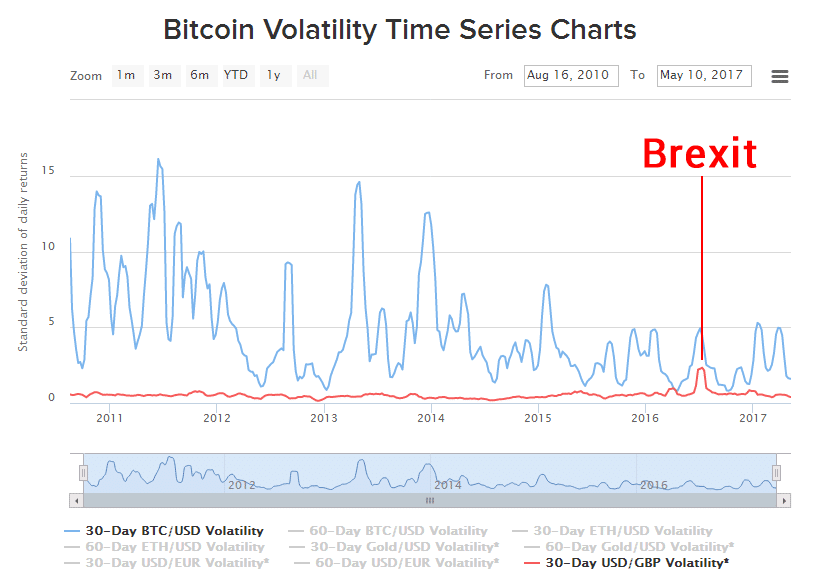
\includegraphics[width=0.6\textwidth]{content/images/BitcoinVolatility}
	\caption{BTC/USDT and USDT/Pound volatility compared.}
	\scriptsize Source: \url{https://99bitcoins.com/bitcoin-volatility-explained}
	\label{fig:bitcoinvolatility}
\end{figure}





%\section{Supervised Learning}
%Supervised learning is a subdomain of machine learning, where a function is learned from labeled training data $\{ (x_1, y_1), ..., (x_N, y_N) \} $. Each training sample maps a feature vector $x_i \in X$ to a desired target value or label $y_i \in Y$. Target values may either be categorial, making the learning task a \emph{classification} problem, or continuous, making the learning task a \emph{regression} problem.\\

%A supervised learning algorithms seeks to find a general function $g_\theta()$ (or it's parameters $\theta$), such that $g_\theta(x_i) \approx y_i | i \leq N$. The learned function should ideally avoid overfitting by finding a generalization to previously unseen data.

%{\color{red}Keep or Remove?! Or Move below \Cref{chap:RLfunctionapproximation}}

%\subsection{Random Forest}
%bla







\section{Reinforcement Learning}
\ac{RL} is a subdomain of machine learning. It was first defined by Sutton and Barto\Cite{Sutton98reinforcementlearning} as the problem of learning from interactions with an environment in order to achieve long-term goals. In contrast to \ac{SuL}, no labeled training data is present, such that sub-optimal actions can not be corrected explicitly. Instead, in each time step $t$, the agent takes the action $a_t$ which maximizes\footnote{Alternatively, it is possible to \emph{minimize} the future expected cost: $C_t = - R_t$} his future expected reward $R_t$, based on empirical knowledge.\\

\Cref{fig:rlagent} shows the typical \ac{RL} scenario. An agent (partially) observes a state $s_t$ and a reward $r_t$ at every discrete time step $t$. It takes an action $a_t$ and hereon receives a new state $s_{t+1}$ and reward $r_{t+1}$.\\


\tikzstyle{block} = [rectangle, draw, 
    text width=8em, text centered, rounded corners, minimum height=4em]
    
\tikzstyle{line} = [draw, -latex]

\begin{figure}[ht]
	\centering
\begin{tikzpicture}[node distance = 6em, auto, thick]
    \node [block] (Agent) {Agent};
    \node [block, below of=Agent] (Environment) {Environment};
    
     \path [line] (Agent.0) --++ (4em,0em) |- node [near start]{Action $a_t$} (Environment.0);
     \path [line] (Environment.190) --++ (-6em,0em) |- node [near start] {New state  $s_{t+1}$} (Agent.170);
     \path [line] (Environment.170) --++ (-4.25em,0em) |- node [near start, right] {Reward $r_{t+1}$} (Agent.190);
\end{tikzpicture}
	\caption{The discrete \ac{RL} scenario defined by Sutton and Barto\Cite{Sutton98reinforcementlearning}.}
	\label{fig:rlagent}
\end{figure}

Rather than learning from labeled training data, the agent applies a \emph{trial and error} pattern and exploits (delayed) external rewards to find actions, maximizing the expected future reward. As actions may not necessarily show an immediate effect, rewards are often delayed and must be accounted for in the so called \emph{credit assignment problem}\Cite{MinskyManuscript-MINSTA}.\\

The expected future reward $R_t$ can be expressed by the cumulative reward of all successive rewards. The discounting factor $\gamma \in [0,1]$ represents the importance between long-term and short-term rewards. With a high $\gamma$, the agent aims to maximize long-term rewards, whereas a small $\gamma$ leads to greedy actions, favouring short-term rewards. 
\begin{equation}
	R_t = \sum_{i=0}^{\infty} \gamma^i r_{t+i+1}
\end{equation}







\subsection{Markov Decision Process}
In reinforcement learning, the environment is typically formulated as \ac{MDP} \Cite{Bel}, which provides a mathematical framework for optimization problems.\\

An \ac{MDP} is a discrete time stochastic control process, written as 5-tuple $(S, A, P, R, \gamma)$. It consists of a (finite) set of environment states $s \in S$, a (finite) set of actions $a_t \in A$, a transition probability matrix $P: S \times A \rightarrow \mathbb{P}(S)$, which maps from state-action pairs $(s_t, a_t)$ to a probability distribution over all successor states $s_{t+1} \in S$,
\begin{equation}
	P^a_{ss'} = \mathbb{P}[s_{t+1}=s' | s_t=s, a_t=a]
\end{equation}

and a reward (or cost) function $R: S \times A \rightarrow \mathbb{R}$, that computes the immediate reward received after applying action $a_t$ in state $s_t$.
\begin{equation}
	R^a_{s} = \mathbb{E}[r_{t+1} | s_t=s, a_t=a] = -\mathbb{E}[c_{t+1} | s_t=s, a_t=a]
\end{equation}

The discount factor $\gamma \in [0,1]$ eventually defines the level of foresightedness. It is obligatory in \ac{MDP}s with an infinite time horizon, to impede infinite values for accumulated long-term returns.\\

The general goal in reinforcement learning is to find optimal policies $\pi^*: S \rightarrow A$, that map states to the best applicable actions, such that the (discounted) expected long-term reward is maximized, or respectively the (discounted) expected long-term cost is minimized.
\begin{equation}
    \pi^*(s) = arg\max_{a \in A(s)} \mathbb{E}[R_t | s_t=s] \>=\> arg\min_{a \in A(s)} \mathbb{E}[C_t | s_t=s]
\end{equation}





\subsection{Markov Property}
An important condition of \ac{MDP}s is the \emph{Markov Property}, which defines the probability distribution of future states to be independent of the past ($s_{t-n}$), given the present ($s_t$). As such, states must capture all relevant information from the history, to deliver sufficient statistics of the future. A state $s_t$ is \emph{Markov} if and only if:
\begin{equation}
     \mathbb{P}(S_{t+1} = s' | s_t, a_t) = \mathbb{P}(s_{t+1} = s' | s_t, a_t, s_{t-1}, a_{t-1}, \ldots{})
\end{equation}






\subsection{Value Function and Bellmann Equation}
In order to find the optimal strategy $\pi^*$, the value of states and actions must be estimated. The state-value function $V^\pi: S \rightarrow \mathbb{R}$ returns the expected reward (or cost) when following $\pi$ from state $s$:
\begin{equation}\label{eq:valuefunction}
\begin{split}
     V^\pi(s) & = \mathbb{E}[R_t | s_t = s] \\
      & = \mathbb{E}_\pi [\sum_{k=0}^\infty \gamma^k r_{t+k+1} | s_t=s] \\
      & = \mathbb{E}_\pi [r_{t+1} + \gamma \sum_{k=1}^\infty \gamma\,^k r_{t+k+1} | s_t=s] \\
      & = \sum_{s' \in S} P(s' \,|\, s, \pi(s))\>[r(s, \pi(s), s') + \gamma\, V^\pi(s')]
\end{split}
\end{equation}

where $0 \leq \gamma \leq 1$ is the discount rate. Assuming an optimal policy $\pi^*$, the optimal value function may be rewritten as $V^{\pi^*} = V^*$ and Bellmann's \emph{principle of optimality} holds:

\begin{quote}
\emph{"An optimal policy has the property that whatever the initial state and initial decision are, the remaining decisions must constitute an optimal policy with regard to the state resulting from the first decision."}

\begin{flushright}
      Richard Bellman, 1957 \cite{bellman1957}
   \end{flushright}
\end{quote}
\begin{equation}\label{eq:bellmanequation}
     V^*(s) = \max_{a \in A}\sum_{s' \in S} P(s' \,|\, s, a)\>[r(s, a, s') + \gamma\, V^*(s')]
\end{equation}

The \emph{Bellman equation} shown in \Cref{eq:bellmanequation} rewrites the value estimation problem as a recursive definition of the value function. This recursion breaks the complex optimization problem into simpler subproblems, that can be solved via \emph{Dynamic Programming}\cite{bellman1957}.





\subsection{Value Iteration}
Bellmanns \emph{value iteration algorithm} recursively applies the Bellman equation to an arbitrarily initialized value function, as shown in \Cref{alg:valueIteration}.  The algorithm repeatedly computes $V^{k+1}$ for all states $s \in S$, until convergence: $\lim\limits_{k \rightarrow \infty}{V^k} = V^*$. In practice, value iteration is stopped, once the Bellmann residual (\ie the difference between both sides of the equation) falls below a predefined threshold $\theta$.\\

\begin{algorithm}[H] 
 \caption{Value Iteration.}
     \SetAlgoLined
         \footnotesize
     
     \KwIn{MDP, $\theta > 0$}
     \KwOut{approximate of $V^*$}
     
     $V^0(s) \leftarrow$ arbitrary values\;
     $k \leftarrow 0$\;
     \Repeat{$\forall s \abs{V^k(s) - V^{k-1}(s)} < \theta$}{
         $k \leftarrow k + 1$\;
      	\ForEach{state $s \in S$}{
        	  $V^k(s) = \max\limits_{a \in A}   \sum\limits_{s' \in S} P(s' \,|\, s, a)\>[r(s, a, s') + \gamma\, V^{k-1}(s')$ \;
      	}
      }

\label{alg:valueIteration}
\end{algorithm}\bigskip

Once the optimal  value function $V^*(s)$ is known, the optimal policy $\pi^*$ can simply be extracted thereof:
\begin{equation}
     \pi^*(s) = \arg\max_{a \in A}\sum\limits_{s' \in S} P(s' \,|\, s, a)\>[r(s, a, s') + \gamma\, V^*(s')]
\end{equation}










\subsection{Q-learning}
A more challenging problem arises, if transition probability matrix $P: S \times A \rightarrow \mathbb{P}(S)$ and reward function $R: S \times A \rightarrow \mathbb{R}$ are unknown a priori. In such case, the \emph{model-free} reinforcement learning technique \mbox{\emph{Q-learning}} \Cite{Watkins:1989} can be utilized to learn an action-value function $Q$, based on previously observed state transitions. The action value function $Q^\pi: S \times A \rightarrow \mathbb{R}$ returns the expected reward (or cost) starting from state $s$, taking action $a$, and following $\pi$ thereafter:
\begin{equation}
\begin{split}
     Q^\pi(s, a) &= \mathbb{E}[R_t | s_t = s, a_t=a] \\
     & = \mathbb{E}_\pi [\sum_{k=0}^\infty \gamma^k r_{t+k+1} | s_t=s, a_t=a] \\
     & = \mathbb{E}_\pi [r_{t+1} + \gamma \sum_{k=1}^\infty \gamma\,^k r_{t+k+1} | s_t=s, a_t=a] \\
     & = \sum_{s' \in S} P(s' \,|\, s, a)\>[r(s, a, s') + \gamma\, Q^\pi(s', \pi(s'))]
\end{split}
\end{equation}

Similar to above, the optimal action-value function may be rewritten as $Q^{\pi^*} = Q^*$:
\begin{equation}
     Q^*(s, a) = \sum_{s' \in S} P(s' \,|\, s, a)\>[r(s, a, s') + \gamma\, \max_{a' \in A}Q^*(s', a')]
\end{equation}

The \emph{Q-learning algorithm}, shown in \Cref{alg:qlearning}, repeatedly computes $Q^{k+1}$ from a set of previously observed transition tuples $D = \{(s, a, r, s'), \dots{}| t=1..n\}$, until convergence: $\lim\limits_{k \rightarrow \infty}{Q^k} = Q^*$. Convergence is guaranteed if all state-actions pairs are visited an unbounded number of times and an appropriate learning rate is chosen \Cite{Watkins92q-learning}. \\

\begin{algorithm}[H] 
 \caption{Q-learning \Cite{Watkins:1989}.}
 
     \SetAlgoLined
     \footnotesize
     
     \KwIn{D=$\{(s, a, r, s'), \dots{}\}$, $\alpha>0$, $\theta > 0$}
     \KwOut{approximate of $Q^*$}
     
     $Q^0(s, a) \leftarrow$ arbitrary values\;
     $k \leftarrow 0$\;
     
     \Repeat{$\forall s\forall a \abs{Q^k(s, a) - Q^{k-1}(s, a)} < \theta$}{
         $k \leftarrow k + 1$\;
      	\ForEach{sample $(s,a,r,s') \in D$}{
        	  $Q^k(s, a) = (1-\alpha) Q_{k-1}(s,a) + \alpha(r + \gamma \max_{a' \in A} Q^{k-1}(s', a'))]$\;
      	}
      }

\label{alg:qlearning}
\end{algorithm}\bigskip

Once the optimal state-action function $Q^*(s, a)$ is known, the optimal policy $\pi^*$ can simply be extracted thereof:
\begin{equation}
     \pi^*(s) = \arg\max_{a \in A} Q^*(s,a)
\end{equation}







\subsection{Exploration}
In environments with a large (or infinite) number of states, is is not feasible to visit all state-action pairs an unbounded number of times. Instead, the environment must be examined at the best possible rate. The agent has to carefully balance between \emph{exploration} and \emph{exploitation}, \ie between testing out previously unknown paths and refining of promising actions. As the latter may get stuck in local optima, exploration helps to find the global optimum.\\

This balancing act can be tackled by a so called $\epsilon$-greedy strategy. With a probability of $p=\epsilon \in [0,1]$ the agent takes a random action and with the remaining probability $q=1-\epsilon$ the agent takes the presumably optimal action, as deduced from his current model. As the agent consolidates his model over time, $\epsilon$ may be slowly reduced.


\subsection{Function Approximation}
\label{chap:RLfunctionapproximation}
In small environments, $V$ and $Q$-values are usually stored in a lookup table. For continuous or (infinitely) large environments function approximators are used to generalize the $V$ and $Q$-functions to previously unseen states-action pairs. Besides scalability towards arbitrarily large environments, this may even speed up the learning process, as earlier experiences are generalized to previously unseen states.\\

More formally $V$ and $Q$ are replaced as follows:
\begin{equation}
     V(s) = \hat{V}(s; \theta)
\end{equation}
\begin{equation}
     Q(s, a) = \hat{Q}(s, a; \theta)
\end{equation}
where $\theta$ refers to function parameters, that must be learned through supervised learning methods\footnote{
Supervised learning is a subdomain of machine learning, where a function is learned from labeled training data $\{ (x_1, y_1), ..., (x_N, y_N) \} $. Each training sample maps a feature vector $x_i \in X$ to a desired target value or label $y_i \in Y$. Target values may either be categorial, making the learning task a \emph{classification} problem, or continuous, making the learning task a \emph{regression} problem.\\
A supervised learning algorithms seeks to find a general function $g_\theta$ (or it's parameters $\theta$), such that $g_\theta(x_i) \approx y_i | i \leq N$. The learned function should ideally avoid overfitting by finding a generalization to previously unseen data.
}.


\subsection{Batch Reinforcement Learning}
\label{chap:basics:batchreinforcementlearning}
In the general reinforcement learning problem, the agent observes a state $s_t$, executes an action $a_t$ and incrementally improves its policy $\pi$ in conformity with the obtained reward $r_t$ and successor state $s'_t$ in an infinite loop. In \emph{batch reinforcement learning} \Cite{Lange_batchreinforcement}, an optimal strategy is learned from a fixed set of known transition samples $D=\{(s,a,r,s'), \dots{}| t=1..n\}$. As shown in \Cref{fig:batchlearning}, the samples are collected a priori in an exploration phase, that is not part of the actual batch learning task.

\begin{figure}[ht]
	\centering
\begin{tikzpicture}[node distance = 16em, auto, thick]
    \node[draw] at (0, 0)   (A) {Exploration};
    \node[draw] at (5.4, 0)   (B) {Learning};
    \node[draw] at (10, 0)   (C) {Application};
    \draw[orange, dashed, line width=0.7mm] (5.4,-0.2) node[minimum height=1.6cm,minimum width=2.2cm,draw, label={above: batch learning}] {} ;
    
    \draw[->] (A) node[above, xshift=2.7cm] {transition set}  node[below, xshift=2.7cm] {$D = \{ (s_t, a_t r_t, s'_t)  \}$} -- (B);

    \draw[->] (B) node[above, xshift=2.1cm] {policy}  -- (C);
\end{tikzpicture}
	\caption{Batch Reinforcement Learning.}
	\label{fig:batchlearning}
\end{figure}

Because exploration has an important impact on the achieved strategy quality, more modern \emph{growing batch reinforcement learning} approaches frequently alternate between exploration and learning phase as shown in \Cref{fig:growingbatchlearning}. In doing so, the agent gets a rough idea of a good policy in order to focus on \emph{interesting} regions of the state space.

\begin{figure}[ht]
	\centering
\begin{tikzpicture}[node distance = 16em, auto, thick]
    \node[draw] at (0, 0)   (A) {Exploration};
    \node[draw] at (5.4, 0)   (B) {Learning};
    \node[draw] at (10, 0)   (C) {Application};
    \draw[orange, dashed, line width=0.7mm] (2.7,-0.6) node[minimum height=2.3cm,minimum width=8cm,draw, label={above: growing batch learning}] {} ;
    
    \draw[->] (A) node[above, xshift=2.7cm] {transition set}  node[below, xshift=2.7cm] {$D = \{ (s_t, a_t r_t, s'_t)  \}$} -- (B);
    \draw[->] (B.south) node[below, xshift=-2.7cm, yshift=-0.7cm] {exploration policy}  -- ++(-0,0) -- ++(0,-0.7) -| (A);
    \draw[->] (B) node[above, xshift=2.1cm] {policy}  -- (C);
\end{tikzpicture}
	\caption{Growing Batch Reinforcement Learning.}
	\label{fig:growingbatchlearning}
\end{figure}

\subsection{Tree-Based Batch Mode Reinforcement Learning}
\label{chap:background:treebasedBatchRL}
Randomized decision trees can be used to approximate the parameters of $Q(s, a; \theta)$, as proposed by Damien Ernst \Cite{Ernst:2005:TreeBasedBatchModeRL}. The batch reinforcement learning algorithm is shown in \Cref{alg:fittedQiteration}.\\

\begin{algorithm}[H] 
 \caption{Fitted Q Iteration \Cite{Ernst:2005:TreeBasedBatchModeRL}.}
     \SetAlgoLined
          \footnotesize
     
     \KwIn{$D=\{  (x_t, a_t, s_t, r_t), \dots{} | t=1..n  \}$}

     $\hat{Q} \leftarrow 0$\;
     $k \leftarrow 0$\;
     \Repeat{stopping condition reached}{
     $k \leftarrow k + 1$\;
      generate pattern set $P = \{(i^t, o^t) | t=1,.., n\}$ where\;
      \Indp    $i^t = (x^t, a^t),$ \hspace{0.7cm}  $o^t = r_t + \gamma * \max\limits_{u} \hat{Q}^k(s_t, u)$\;
      \Indm $\hat{Q}^{k+1} \leftarrow ^{fit} P$
     }
\label{alg:fittedQiteration}
\end{algorithm}\bigskip


\section{Optimized Trade Execution}
As outlined in \Cref{chap:objectives}, the problem of \emph{optimized trade execution} is defined by a particular financial instrument, which must be bought or sold within a fixed time horizon, while minimizing the expenditure (share price) for doing so. In order to achieve the best possible price, proper timing is crucial to reduce hidden costs like slippage (see \Cref{chap:slippage}).\\

The general task of this work is to apply reinforcement learning to successfully learn state-based strategies for optimal order placements. Based on the observed market situation and trade progress the obtained \acl{SR} (see \Cref{chap:tradingstrategies}) may become more or less aggressive as time passes.\\

The examined agents derive their strategies from a (growing) batch of sample transitions stemming from interactions with a simulated trading environment, that is described in the next chapter.




\cleardoublepage{}
\chapter{Orderbook Trading Simulator}
\label{chap:simulator}
As reinforcement learning requires agents to interact with an environment, a trading simulation framework is implemented. The accrued \acf{OTS} provides a full-featured reinforcement learning environment, that simulates the execution of orders on historic data and returns vital feedback to steer the agent towards optimal decisions. Additionally, it serves as a backtesting framework in order to evaluate the cost reducing capabilities of different trading strategies.\\

This chapter describes the origin and quality of the assessed orderbook data, as well as the \ac{OTS} and it's underlying OrderbookContainers.


\section{Data Origin}
\label{chap:dataorigin}
Since typical financial data providers must make an earning from their treasures, they typically only deliver delayed market data on a complimentary basis. Investors dependent on real time or level 2 market data (see \Cref{sec:marketdata:levels}) are usually charged horrendous monthly subscription fees.\\

A costless alternative exists in open cryptocurrencies, like bitcoins (see \Cref{chap:bitcoins}). The digital asset exchange platform Poloniex \footnote{\url{http://www.poloniex.com}} provides an open API for querying detailed market data in real time. As their push API, to receive live order book updates and trades, was rather error-prone and buggy when this project started, the decision was made, to query full orderbooks on a minutely basis.\\

On Nov, 10th 2016, 10:00 am, a daemon was started, to fetch orderbook snapshots up to a market depth of $5.000$ from Poloniex via HTTP GET requests (see \Cref{lst:PoloniexFetch}). The volume of recorded orderbook snapshots for nine distinct currency pairs\footnote{Recorded currency pairs include USDT/BTC, BTC/ETH, BT/XMR, BTC/XRP, BTC/FCT, BTC/NAV, BTC/DASH, BTC/MAID, BTC/ZEC} has since grown to roughly 100GB (as per 2017-06-20). This thesis is based on a condensed version of the currency pair USDT/Bitcoin.

\begin{lstlisting}[frame=single, breaklines=true, basicstyle=\scriptsize, caption=Data fetched from Poloniex via HTTP GET request, label=lst:PoloniexFetch]
# https://poloniex.com/public?command=returnOrderBook&currencyPair=USDT_BTC&depth=5000
{"asks" :[[ "705.450000" ,2.772181], [ "705.450196", 0.139212] ,["706.170000" ,0.052838] , ... ], "bids":[["705.000000",0.158232],["703.700000" ,0.001250], ... ], "isFrozen": 0, "seq": 63413296}
\end{lstlisting}

\begin{figure}[ht]
	\centering
   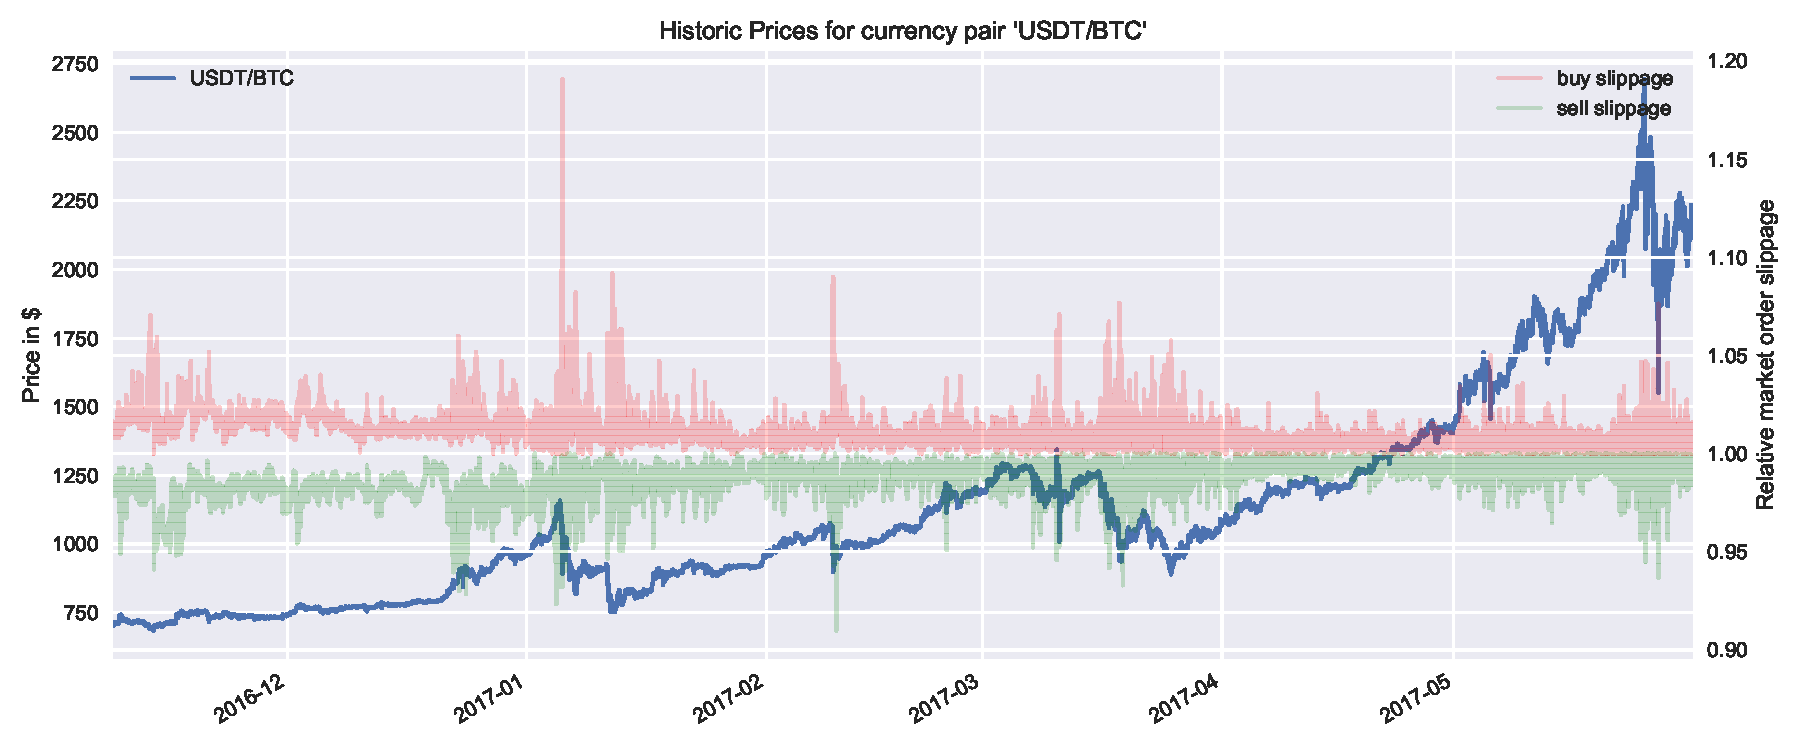
\includegraphics[width=1.\textwidth]{content/drawings/bitcoin_historicPrices}
	\caption{Historic center prices between Nov, 10th 2016 and May, 31 2017, as fetched from Poloniex.}
	\label{fig:ploniexPriceHistory}
\end{figure}

\Cref{fig:ploniexPriceHistory} shows the price evolution of currency pair USDT/Bitcoin over the period of recording. Prices have burst from roughly $700\$$ to more than $2.000\$$. Red and green lines depict the relative difference between the worst price paid/received for an immediate market order of $\pm70.000\$$ respectively\footnote{With a total trading volume of roughly $40.000.000\$$ per day (see \Cref{chap:bitcoin:volatility}), these $\pm70.000\$$ refer to roughly $4.2\%$ thereof.}.

\hspace{1cm}

\section{Data Preprocessing}
\label{chap:preprocessing}
The python \lstinline!class OrderbookContainer! aggregates all informations contained in an individual orderbook snapshot. It enforces correct price ordering in the two opposing bid and ask books and provides additional methods for market visualization and feature extraction. To restrict wasteful memory usage, orderbook snapshots are condensed in several ways:

\begin{itemize}
\item Almost identically price levels are round to the second decimal and their respective order volumes merged.

 \[ 
  \begin{rcases}
    0.139212 * 705.450000\\
    2.632969 * 705.450196\\
  \end{rcases} 
  = 2.772181 * 705.45
\]
\item Market depth is capped just above the threshold of 100 bitcoins, roughly corresponding to a market depth of 100-140 prices levels in both books. This threshold allows to simulate trades up to a market order price of $70.000\$$ at any time throughout the whole recording period.

\item Erroneous orderbook snapshots have been discarded. Occasional errors may occur, due to Poloniex API failures.

\end{itemize}

These measurements reduce the average individual orderbook snapshots size from 30KB to approximately 6.6KB. As for the december 2016, this results into $44.640$ snapshots with a total size of 295MB instead of 1.35GB, clearly reducing the memory consumption.\\

\Cref{lst:OrderbookContainer} shows the most important functions, provided by the OrderbookContainer class. OrderbookContainer instances are vigorously used by the \ac{OTS}. \Cref{fig:orderbook} shows a plain visualization of an individual orderbook snapshot.

\begin{lstlisting}[frame=single, breaklines=true, basicstyle=\scriptsize, caption=OrderbookContainer, label=lst:OrderbookContainer]
ob = OrderbookContainer(timestamp="2016-11-08T10:00",
                        bids=pd.DataFrame([200., 100., 300.],
                        columns=['Amount'], index=[28.7, 28.5, 28]),
                        asks=pd.DataFrame([25., 50., 200.],
                        columns=['Amount'], index=[29., 30., 31.]))
# Available methods
ob.plot(outfile='sample.pdf')  # plt.show or plt.savefig
ob.asks  # pd.DataFrame
ob.bids  # pd.DataFrame
ob.features  # returns a dict of precomputed features
ob.get_bid(), ob.get_ask(), ob.get_center()  # float
ob.get_current_price(volume=100)  # achievable cashflow by market order
ob.get_current_sharecount(cash=70000) # number of shares aquirable by market order
ob.compare_with(other_ob) # returns orderbook deltas used by the OTS
ob.enrich()  # computes Volume, VolumeAcc and norm_Price
ob.head(depth=3)  # returns the orderbook, capped at a market depth of 3
ob.plot()
\end{lstlisting}


\begin{figure}[ht]
	\centering
   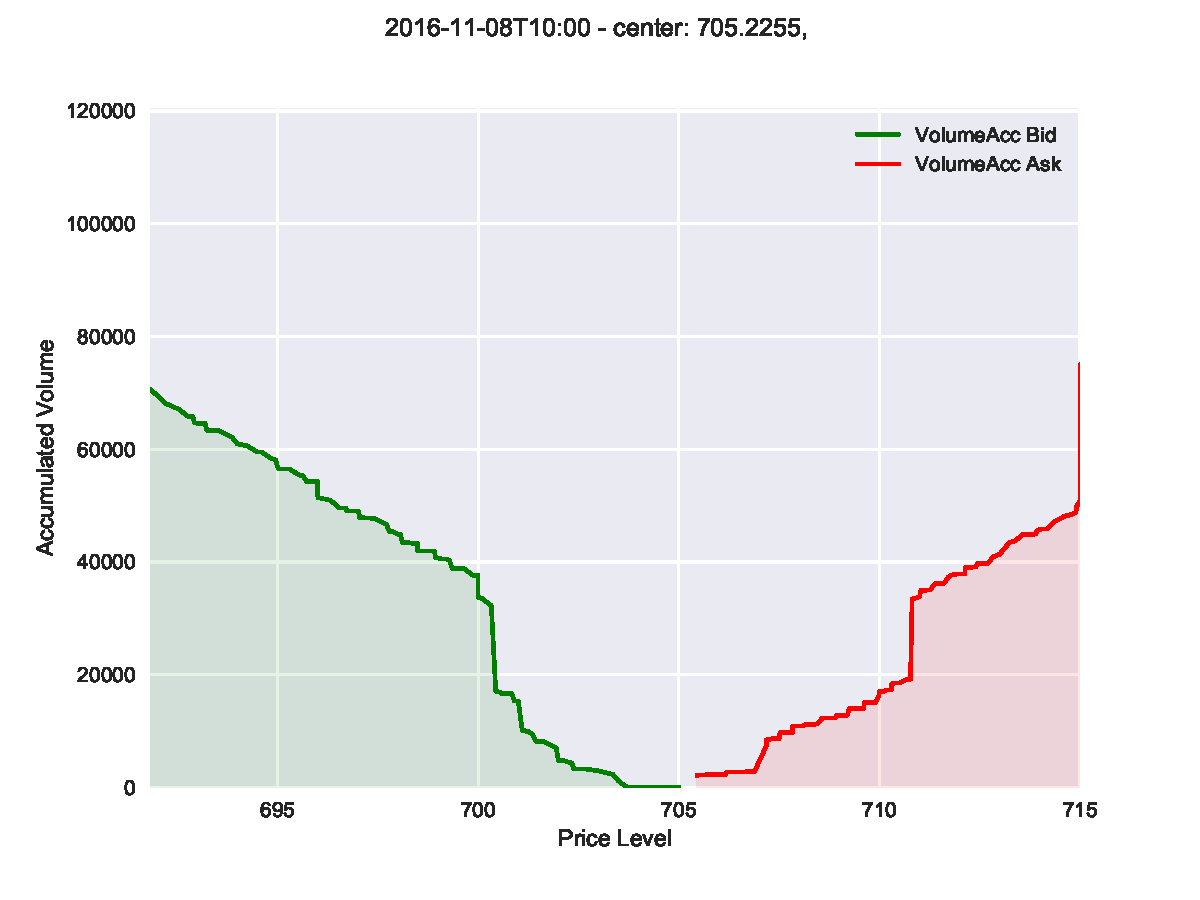
\includegraphics[width=0.7\textwidth]{content/drawings/orderbook}
	\caption{A simple visualization of an limit orderbook.}
	\label{fig:orderbook}
\end{figure}


\section{Simulator}
The \ac{OTS} framework serves as base for all preceding experiments and evaluations.
Each simulator instance is fed with an array of subsequent OrderbookContainers (\emph{orderbook windows}) and a targeted trading volume $V$, which it pretends to trade into cash or vice versa within a fixed time horizon $H$, according to an external strategy.\\

In the rare case of missing orderbook snapshots (see \Cref{chap:preprocessing}), the \emph{real} time horizon may be larger than usual, since always $H$ subsequent orderbooks are selected. By default, the \ac{OTS} refuses to work with orderbook windows, whose actual length differs from the presumed length by more than two minutes.\\

Limit orders may be placed at predefined, discrete time steps within the trading horizon $H$. This is done through the simulators main interface method \lstinline!trade(limit=...)!. The simulator is done, once the remaining trading volume is zero, which is enforced at the very last time point. Any remaining volume at $H-1$ is transformed into a simple market order and executed immediately, at any price. Additional parameters control the simulators precise behavior:

\begin{description}
\item[volume] : The targeted trading volume $V$.\\
Positive values indicate buy orders, negative values indicate sell orders.
\item[consume] : \lstinline!'cash'! or \lstinline!'volume'!\\
Defines whether \lstinline!volume! should be interpreted as \emph{cash} (goal: buy/sell shares for $V$ dollars), or as \emph{sharecount} (goal: buy/sell $V$ shares).
\item[period\_length] : \lstinline!default=15!\\
Defines the duration at which a limit order is executed. After a trade has been placed, the simulator iterates over the next \lstinline!period_length! orderbooks, before the results are reported and a reviewed order may be placed.

\item[tradingperiods] : \lstinline!default=4!\\
Defines the number of trade reviews, that can be made within the time horizon $H =$ \lstinline!period_length * tradingperiods!.

\item[max\_lengh\_tolerance] : \lstinline!default=2!\\
Defines the accepted tolerance between actual and presumed trading horizon in minutes. Throws \lstinline!ValueError!, if exceeded.

\item[costtype] : \lstinline!default='slippage'!\\
Defines which of multiple cost functions to use in the reports returned. 
\end{description}

\subsection{Orderbook and strategy visualization}

\Cref{fig:orderbookwindow} visualizes a 60 minutes long orderbook window, where the solid red lines mark the \emph{average} (\ref{fig:orderbookwindow:avg}) and \emph{worst} (\ref{fig:orderbookwindow:worst}) price, that has to be paid at a given time point, in case of an immediate market order of $100$, $75$, $50$ and $25$ bitcoins respectively. Analogously, the solid green lines represent achieved prices for sale orders of $-25$, $-50$, $-75$ and $-100$ bitcoins respectively.\\

As can be seen in this graph, ask prices (red) deviate slightly more from the center price than bid prices (green) do. An plausible inference is, that imbalances between demand and supply might serve as a valuable indicator for future price trends.

\begin{figure}[ht]
	\centering
	\begin{subfigure}[t]{0.5\textwidth}
        		\centering
        		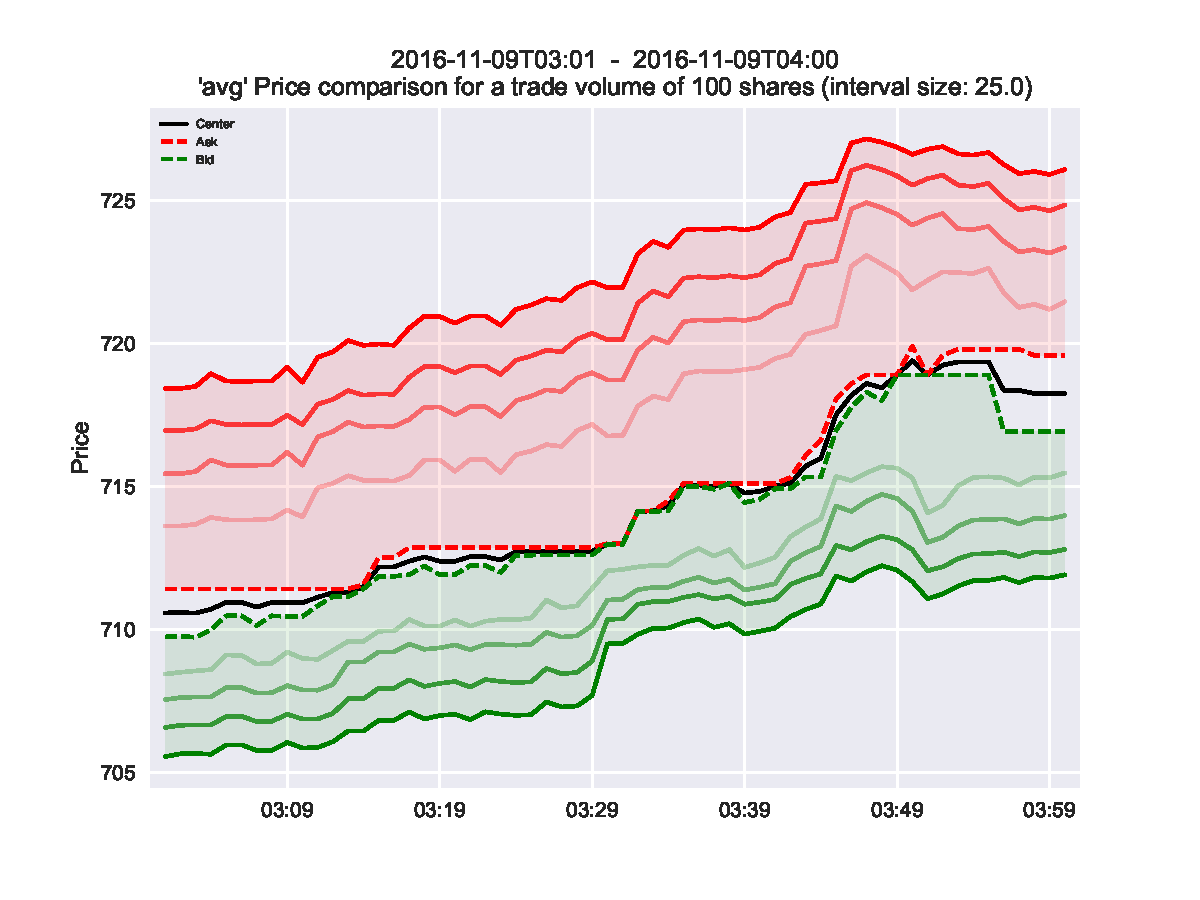
\includegraphics[width=\textwidth]{content/drawings/orderbook_window17}
        		\caption{Average market price.}
		\label{fig:orderbookwindow:avg}
    	\end{subfigure}%
	\begin{subfigure}[t]{0.5\textwidth}
        		\centering
        		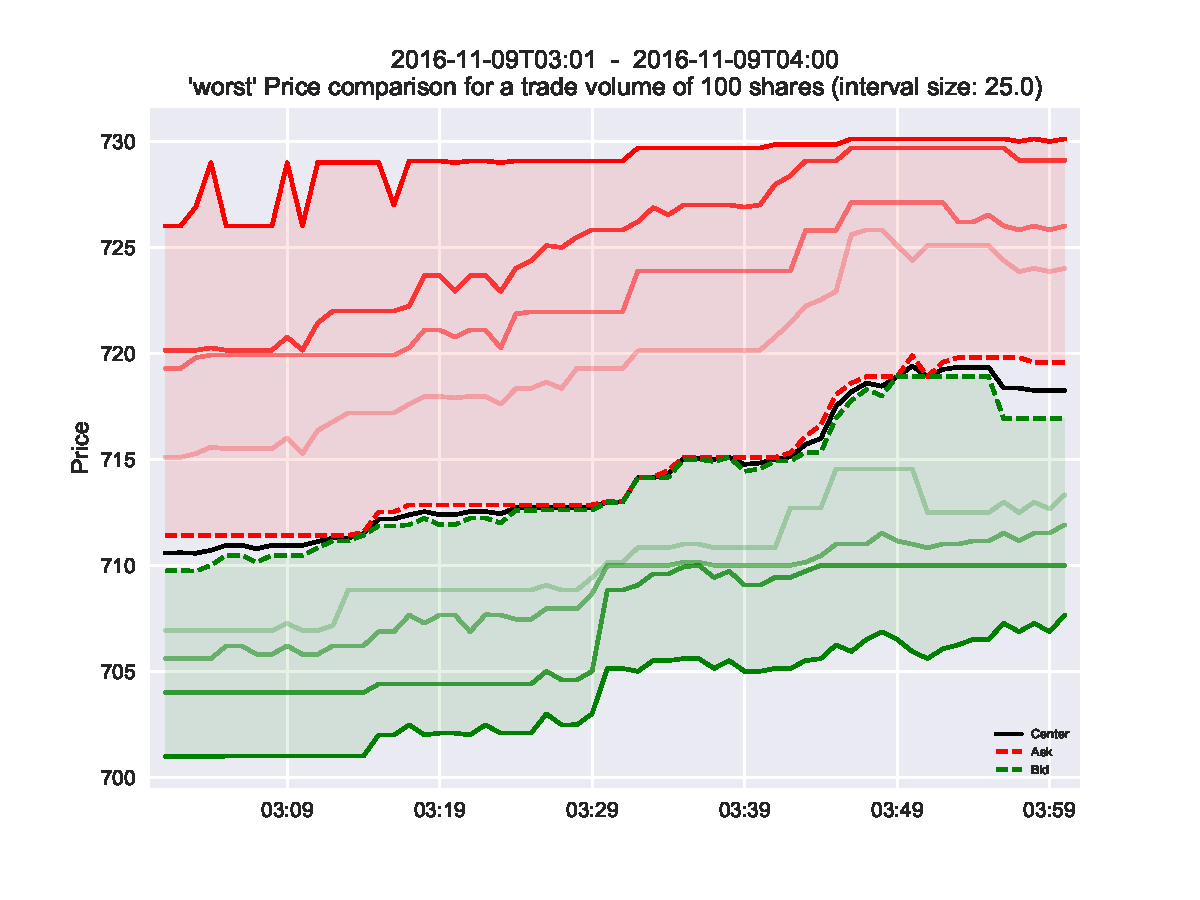
\includegraphics[width=\textwidth]{content/drawings/orderbook_window17_worst}
        		\caption{Worst market price.}
		\label{fig:orderbookwindow:worst}
    	\end{subfigure}%
	
	\caption{An orderbook window over a period of 60 minutes.}
	\label{fig:orderbookwindow}
\end{figure}

\subsection{Masterbook}
During instantiation, the \ac{OTS} creates a copy of the first orderbook, called the \emph{masterbook}. Hereinafter, executed trades do only affect this internal \emph{masterbook}. The remaining orderbooks are then converted into \emph{deltabooks}, containing only changes between subsequent orderbooks.\\

The \ac{OTS} may be reset to its initial state at any time via \lstinline!ots.reset()!. This avoids computational overhead, when testing out multiple strategies on the same \emph{window}, as only \emph{masterbook} and \emph{history} are reset, while \emph{deltabooks} need not be recomputed and \emph{orderbooks} need not be retransferred. \lstinline!ots.reset()! provides optional parameters for modifying the simulators start conditions. As such the simulator might be instructed to start at a \lstinline!custom_starttime! or with a \lstinline!custom_startvolume!, to simplify the exploration of possible strategies.

\subsection{Trade execution}
\label{chap:tradeexecution}
The simulated trade execution is triggered by an external call to \lstinline!trade(limit=...)!. The \ac{OTS} expects a \lstinline!limit! and iterates over the next \lstinline!period_length! orderbooks, matching all eligible orders. The \lstinline!limit! represents the highest accepted price level for buy orders and the lowest accepted price level for sell orders respectively. If \lstinline!limit=None!, a simple market order is performed.\\

In a first step, all eligible orders, bound by the given limit and the total trade\_volume, are cut from the internal masterbook and pasted into the \lstinline!ots.trade_history!, as such these orders are assumed be fulfilled. The \lstinline!volume! and \lstinline!cash! variables are updated accordingly.
The simulator then moves to the next time point and adds the corresponding \emph{deltabook} to the masterbook.\\

In case of order size reductions\footnote{Order size may be reduced due to order fulfillment, order updates or order cancelations through the other market participants.}, negative order sizes may appear in the masterbook. They are silently dropped, assuming they where matched before they actually vanished from the market. This is a possible source of trouble, as this assumption can not be proven to be valid. As such, matching orders that are simultaneously updated to another price level, are virtually doubled. They are perceived as a new order, even though the responsible market participant has already realized an execution and no basis to submit another one.\\

\begin{figure}[ht]
	\centering
	\begin{enumerate}
	\item \lstinline!master += diff(ob[t] - ob[t-1])!, drop negative share counts.
	\item perform trade: buy until given limit
	\item \lstinline!master -= bought bitcoins!
	\item done if \lstinline!volume==0! or $t==T-1$ (\lstinline!forced=True! a)
	\end{enumerate}
	\caption{The circuit of masterbook adjustments}
	\label{fig:masterbookadjustments}
\end{figure}

The masterbook is then ready to be queried again. Any eligible \emph{new} orders are cut from the masterbook and past into the \lstinline!ots.trade_history!. After \lstinline!period_length! steps, a detailed trading report, as shown in \Cref{tab:tradinghistory} is returned. The upper case columns represent internal variables and orderbook statistics observed at the particular period start. The lower case columns summarize the actual trade in terms of highest, lowest and average price achieved, traded volume, cash flow and observed costs.\\

\begin{table}
\centering
\scalebox{0.44}{
\rowcolors{1}{}{black!5}
\begin{tabular}{|lrrrrrrrrrrrrlrrrr|}
\toprule
{} &     ASK &     BID &  CENTER &  SPREAD &  LIMIT &   T &  VOLUME &  volume\_traded &      CASH &  cash\_traded & ... &     avg & forced &  initialMarketAvg &     low &    high &  cost \\
\midrule
03:01 &  711.42 &  709.74 &  710.58 &    1.68 &  713.0 &  15 &  100.00 &          46.77 &      0.00 &    -33280.72 & ... &  711.51 &  False &            718.42 &  711.42 &  713.00 &     43.48 \\
03:16 &  712.52 &  711.86 &  712.19 &    0.66 &  715.0 &  15 &   53.23 &          28.90 & -33280.72 &    -20630.99 & ... &  713.99 &  False &            718.42 &  712.52 &  715.00 &     98.53 \\
03:31 &  715.10 &  712.98 &  714.04 &    2.12 &  717.5 &  15 &   24.33 &           6.68 & -53911.71 &     -4780.95 & ... &  716.16 &  False &            718.42 &  715.10 &  717.41 &     37.28 \\
03:46 &  718.60 &  717.77 &  718.18 &    0.83 &  720.0 &  15 &   17.65 &          17.65 & -58692.66 &    -12706.15 & ... &  719.73 &  False &            718.42 &  718.60 &  720.00 &    161.57 \\
\bottomrule
\end{tabular}}
\caption{Trading history, as returned after four consecutive calls of \lstinline!ots.trade()!.}
\label{tab:tradinghistory}
\end{table}

\subsection{Visualization}
A visual representation of the same trading strategy, which underlies \Cref{tab:tradinghistory}, is shown in \Cref{fig:tradingstrategy17good}. Here, the \ac{OTS} was instructed to buy $100$ bitcoins within a period of $60$ minutes and called with four consecutive limits prices $713$, $715$, $717.5$ and $720$, which are shown as grey step function in the upper subplot.\\

The second subplot displays trade executions and declining trade volume over time and the bottom subplot displays induced costs. Expected costs conform to the respective accumulated costs, extrapolated to the full trade volume.


\begin{figure}[ht]
	\centering
   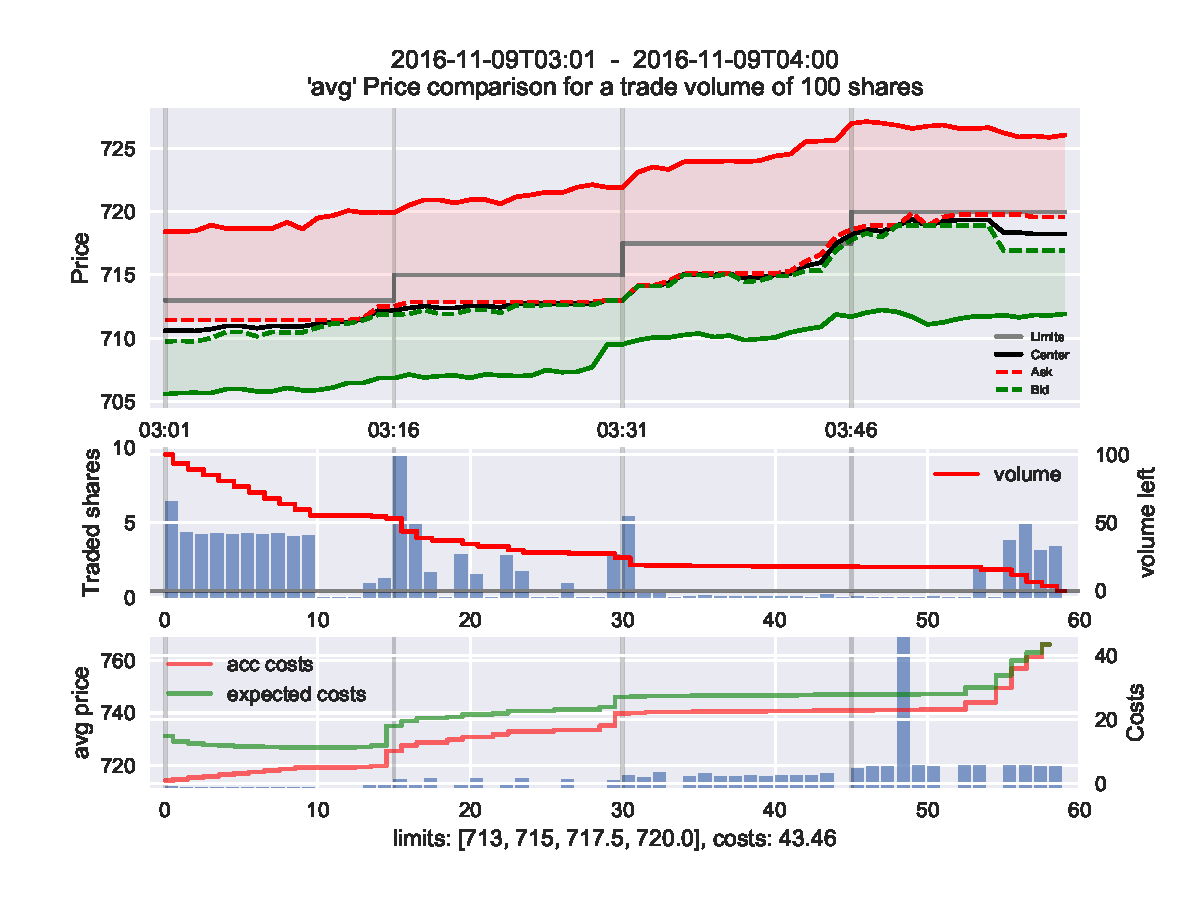
\includegraphics[width=0.8\textwidth]{content/drawings/trading_example17_good}
	\caption{Visualization of an exemplary trading strategy.}
	\label{fig:tradingstrategy17good}
\end{figure}

A total slippage of $340.86\$$ was generated, whereas a simple market order would have cost $784.32\$$.


\subsection{Model correctness}
\label{chap:modelcorrectness}
The presented model does not account for market reactions, induced by the currently executed trading strategy. It moronically follows the market trend, as it would have evolved without any intervention. Some sources of troubles are pictures below:

\begin{itemize}
\item As stated in \Cref{chap:tradeexecution}, the presented model can not distinguish between a limit order being removed from the market makers orderbook and a limit order essentially only being updated to another price level. In the latter case, the order presumably wouldn't have reappeared in the orderbooks after the simulator matched it.
\item Other market participants typically monitor market activity thoroughly, which is particularly true for purely electronic markets of digital assets, like bitcoins. It is delusive to assume, that no other market participants or trading bots react to large orders, that eat significantly into the orderbook.

%\begin{figure}[ht]
%	\centering
%	[placeholder]
%	\caption{Sample of a \emph{curious masterbook shape}.}
%	large part of order fulfilled, eaten deeply into the orderbook, deltabook brings in new orders close to original centerprice $\Rightarrow$ uncommon gap.
%	\label{fig:masterbook:curiousshape}
%\end{figure}

\item Orderbooks on a minutely basis miss a great part of the markets volatility. \\
In addition to orderbook snapshots, professional data providers typically grant access to market level 2 data (see \Cref{sec:marketdata:levels}) in form of log files as well. The log files consist of timestamped orderbook updates (typically of type \emph{remove} and \emph{modify}), which allow the reconstruction of the orderbook for an arbitrary time point. As mentioned in \Cref{chap:dataorigin}, Poloniex push API, to receive live order book updates and trades, was rather error-prone and occasionally failed to report important orderbook updates. As the valid reconstruction of orderbooks is highly vulnerable to missing logs, inconsistencies arose and the decision was made, to query orderbooks on a minutely basis only.
\item Hidden Orders, as introduced in \Cref{chap:ordertypes}, are not accounted for.
\end{itemize}

As a consequence, trading on the masterbook can only be seen as an rough approximation of true market behaviour. Curious masterbook shapes, resulting from the described simulation process, encourage to perform actual feature extraction on the original orderbooks, examining the market as it would have evolved without any interventions.







\cleardoublepage{}
\chapter{Reinforcement Learning Approach}
\label{chap:reinforcementlearning}
This chapter describes a \ac{RL} approach, used to tackle the important problem of optimized trade execution. To a large extend, it is based on the \ac{RL} formulation, as described by Nevmyvaka \etal \cite{Nevmyvaka:2006}. Q-learning and dynamic programming are fused to find an optimal, state-based strategy from a training set of historic orderbook data. Sampling the discretized state space\footnote{The state space describes actual trade progress (\ie \emph{remaining time} and \emph{remaining inventory}) as well as current market situation.} in a brute force manner, the authors achieved an impressive 50\% gain over the more simple Submit \& Leave Strategy (see \Cref{chap:tradingstrategies}).\\

Some of the assumptions made in the original approach deserve a discussion and leave room for potential improvements. As their work was based on a rather large, proprietary dataset of 1.5 years of millisecond time-scale limit order data from \acs{NASDAQ}, it was furthermore intriguing to evaluate its performance on a smaller, self-recorded dataset of limited resolution.


\section{General Framework}
\label{chap:reinforcementlearning:original}
In the first place, the general framework of the reinforcement learning problem is described.


\subsection{State space}
\label{chap:statespace}
The state space consists of various variables, describing the current trade progress (\emph{private variables}) and the current market situation as observable from orderbook data (\emph{market variables}). The two private variables \emph{remaining time} (\lstinline!time!) and \emph{remaining inventory} (\lstinline!volume!) make the base for all subsequent experiments, while optional market variables may be enclosed to potentially assist the process of decision finding.\\

Each \lstinline!state! $s \in <time, volume ,o_1, o_2, ...>$ forms a vector of at least both private variables, plus a variable number of market variables. More specifically, the following market variables were evaluated in terms of improvement over a state space based on two private variables only.
\begin{description}
\item[Bid-Ask Spread]: spread between best bid price and best ask price.
\item[Bid-Ask Volume Misbalance]: volume imbalance between orders at the best bid price and the best ask price.
\item[Immediate Market Order Cost]: costs, if remaining volume would be executed immediately, at the current market price.
\item[Signed Transaction Volume]: signed volume of all trades executed within last 15 seconds. A positive value indicates more buy orders, while a negative value complies to more sell orders being executed.
\end{description}

In the original approach, market variables were discretized into 0 (low), 1 (medium) and 2 (high), while the concrete category mapping process was not further described. Market variables are extracted from the original orderbooks, as if the market had evolved without our impact. Private variables where discretized in 4 to 8 bins, while greater resolutions led to strictly better results and linearily higher computation times.

\subsection{Action space}
\label{chap:actionspace}
Actions define the level of trading aggression to be performed. In the original approach, action $a \in \mathbb{R}$ defines the deviation between current best price and chosen limit price, as $bid + a$ (for buy orders) and $ask - a$ (for sell orders). As such, actions must cross the full bid-ask-spread to find matching orders in the opposing book. Large actions $a$ result in larger fractions of the order volume being matched immediately. Smaller or even negative actions $a$ help to prolong the actual execution, and may help to profit from opportune market movements.\\

In case of the market situation as shown in \Cref{table:orderbook:example:again}, a buy order with an aggressive action $a=1.4$ would map into $limit=bid+a=28.7+1.4=30.1$. This limit would allow trading up to 75 shares instantaneously.\\

\begin{table}
\centering
	\scalebox{0.8}{
\rowcolors{1}{}{black!5}
\begin{tabular}{|RRcRRR|}
\toprule
{} &  \text{Amount} &    Type &  \text{Volume} &  \text{VolumeAcc} &  \text{norm\_Price} \\
\midrule
31.00 &   200.0 &     ask &  6200.0 &     8425.0 &    1.074533 \\
30.00 &    50.0 &     ask &  1500.0 &     2225.0 &    1.039871 \\
29.00 &    25.0 &     ask &   725.0 &      725.0 &    1.005208 \\
28.85 &     NaN &  center &     NaN &        NaN &         NaN \\
28.70 &   200.0 &     bid &  5740.0 &     5740.0 &    0.994810 \\
28.50 &   100.0 &     bid &  2850.0 &     8590.0 &    0.987877 \\
28.00 &   300.0 &     bid &  8400.0 &    16990.0 &    0.970546 \\
\bottomrule
\end{tabular}
}
\caption{Action $a=1.4$ translates into $limit=28.7 + 1.4 = 30.1$.}
\label{table:orderbook:example:again}
\end{table}

The employed number of selectable actions and their actual value range was not further specified.


\subsection{Costs}
\label{chap:costs}
Costs are defined as the slippage induced from the previously chosen actions. The baseline is given by the initial center price. The following formula is used to compute (partial) costs in terms of price deviation from the idealized case of buying all shares at the initial center price:
\begin{equation}
\label{eq:imcost}
   cost_{im} = (avg\_paid - initial\_center) * volume\_traded
\end{equation}
\begin{equation}
   initial\_center = (\dfrac{ask_t+bid_t)}{2} | t=0
\end{equation}

Since the complete trade execution happens within a finite time horizon and full execution of the \lstinline!volume! is mandatory, partial costs can simply be summed up without any discounting. Utilizing the \ac{OTS}, it is not possible to compute occurring costs in advance exactly, as they depend on how the market evolves within the subsequent \lstinline!trading_period!.


\section{Backward learning}
\label{chap:backwardlearning}
In order to learn the optimal limit for each possible situation, orderbook windows are examined in a backward, brute-force manner as described in \Cref{alg:bruteforce:pseudocode}. Each orderbook window from the training data set is sampled $T*I*L$ times, where $T$ is the number of performed limit revisions, $I$ is the number of discrete volume states and $L$ is the number of available actions.\\

\begin{algorithm}[H] 
 \caption{Optimal\_strategy, as described in \Cite{Nevmyvaka:2006}.}
     \SetAlgoLined
     \footnotesize
     
     \KwIn{V=70.000\$, H=60min, T=4, I=[12.5\%..100\%], L=[-4..10]}

\For{t=1 to T}{
    \While{not end of data}{
        Transform (orderbook) $\rightarrow o_1..o_R$\;
        \For{i=0 to I}{
            \For{a=0 to L}{
                 Set $x = [t, i, o_1, ..., o_R]$\;
                    Simulate transition $x \rightarrow y$\;
                    Calculate immediate $\text{cost}_{im}(x, a)$\;
                    Look up argmax $\text{cost}(y, p)$\;
                    Update $\text{cost}([t, v, o_1, ..., o_R], a)$\;

            }
        }
        Select the highest-payout action argmax $\text{cost}(y, p)$ in every state $y$ to output optimal policy
    }
}
\label{alg:bruteforce:pseudocode}
\end{algorithm}\bigskip

While the algorithms running time depends solely on the resolution of the two private variables, the chosen action space and the size of the training data set, it is approximately independent of the number of market variables chosen. The precise transition simulation was not further described, but for this thesis the model described in \Cref{chap:tradeexecution} is utilized. The cost update rule is given below: 
\begin{equation}\label{eq:costfunction}
   cost(x_t, a) = \dfrac{n}{n+1} cost(x_t, a) + \dfrac{1}{n+1} [cost_{im}(x_t,a) + \arg\min_{p}cost(x_{t-1}, p)]
\end{equation}

The algorithm assumes the individual trading\_periods to be of an (approximately) Markovian nature, where the optimal action to choose at state $x_t$ with $t = \tau$ is completely independent of actions chosen previously ($t \geq \tau$).\\

As such, the state-action function can be computed inductively via dynamic programming. In a first round, expected costs for all actions in states being immediate predecessors of end states (\ie $t=1$) are computed according to \Cref{eq:costfunction}. \Cref{fig:heatmap:t1} visualizes the resulting optimal costs (right) and corresponding actions (left) after the first round has finished.

\begin{figure}[ht]
	\centering
   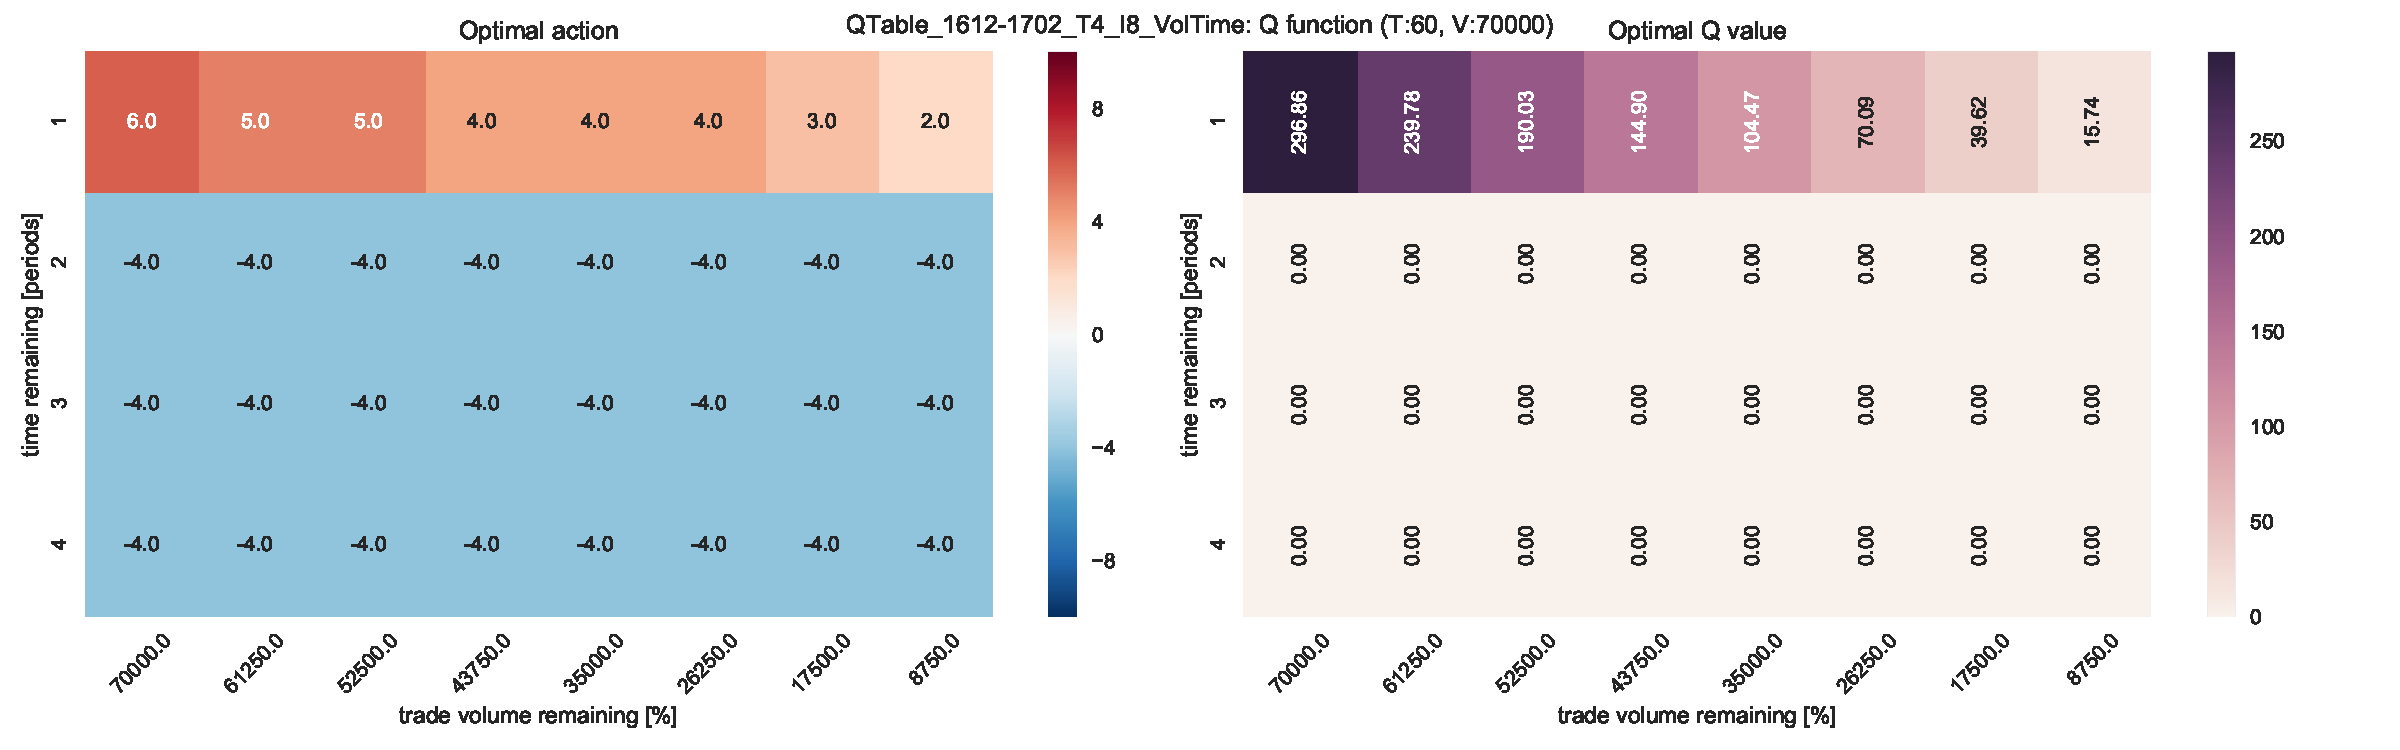
\includegraphics[width=0.8\textwidth]{content/drawings/heatmap_3months_t1}
	\caption{State-Action function, visualized after the first training round.}
	$T=4$, $I=8$, L=15
	\label{fig:heatmap:t1}
\end{figure}

Knowing the optimal state-action values for all states with $t=1$, all informations are given to compute the optimal state-action values for their predecessor states with $t=2$ (see \Cref{fig:heatmap:t2}).

\begin{figure}[ht]
	\centering
   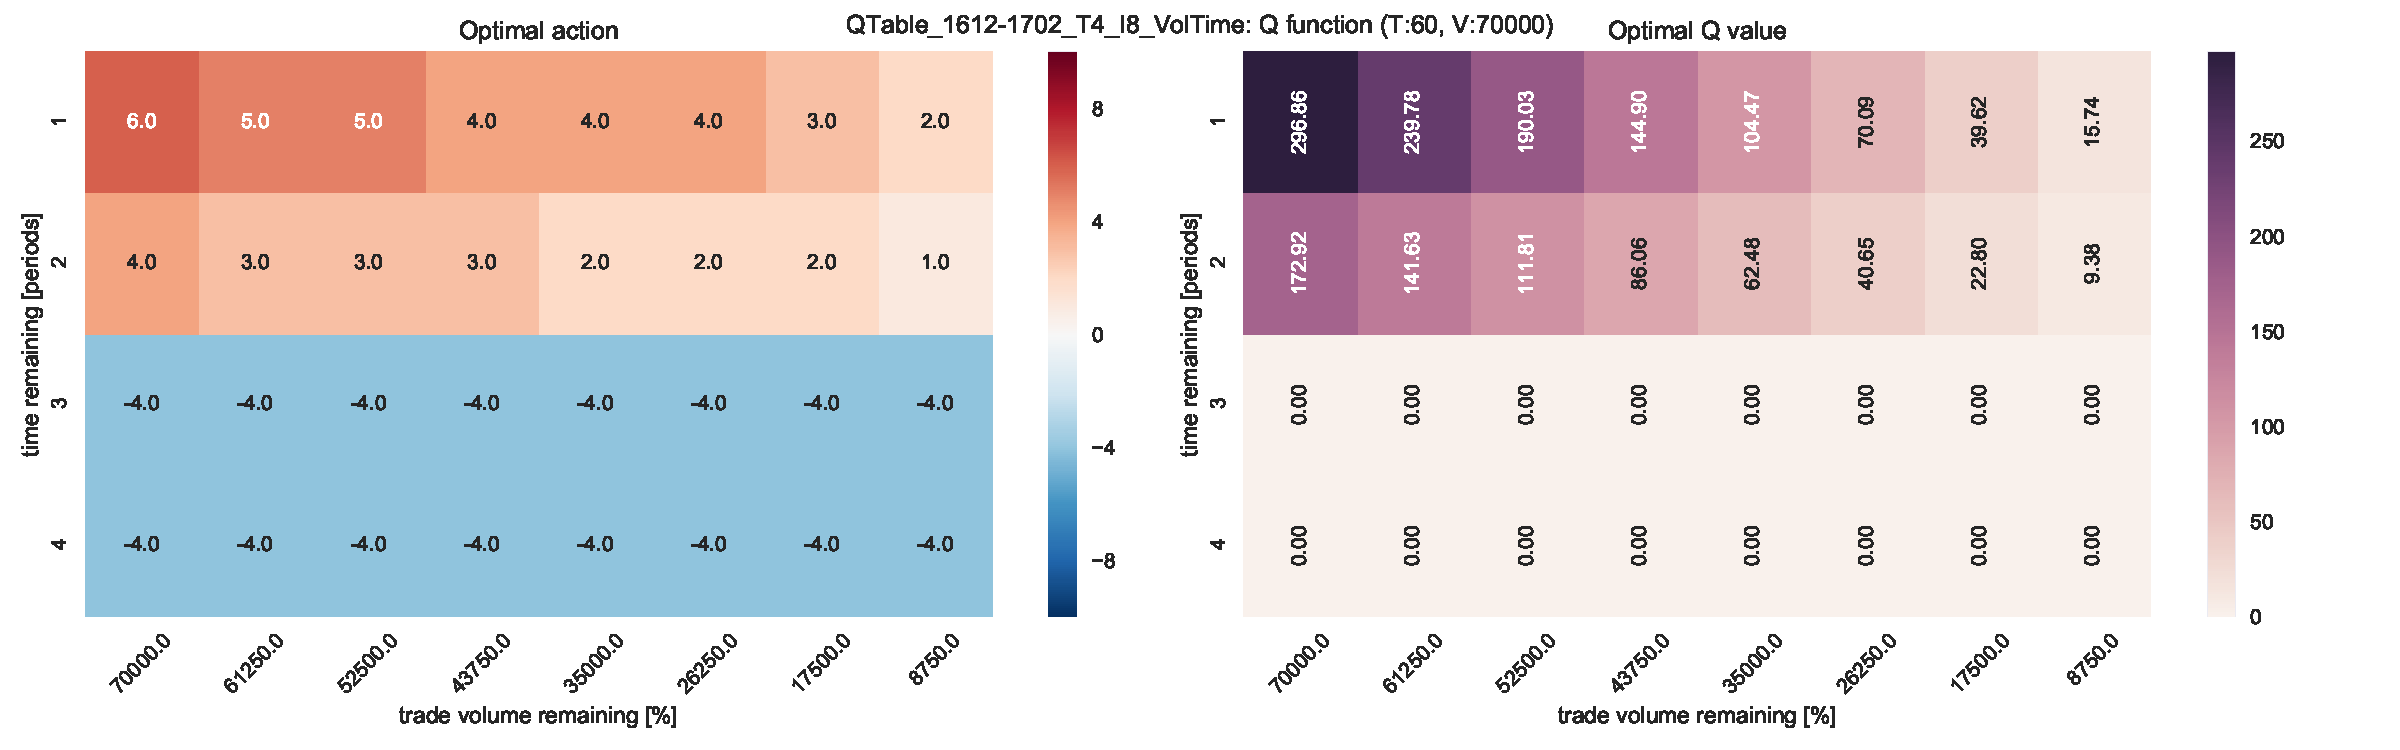
\includegraphics[width=0.8\textwidth]{content/drawings/heatmap_3months_t2}
	\caption{State-Action function, visualized after the second training round.}
	$T=4$, $I=8$, L=15
	\label{fig:heatmap:t2}
\end{figure}

After $T$ iterations a globally optimal policy, as shown in \Cref{fig:heatmap}, has been found. The annotated q values (right) denote the corresponding minimum over all available actions. The visualized state-action function was trained over orderbook snapshots from Nov, 10th 2017 10am to May, 31st 2017, partitioned into 4.154 orderbook windows of 60 minutes length each. Over a trading horizon of $T=4$ \lstinline!trading_periods!, $70.000\$$ cash (discretized in $I=8$ intervals) had to be traded into Bitcoins. The state space included the two private variables \lstinline!time! and \lstinline!volume! only, while the action space comprised $L=15$ actions. As such, a total of $4.154 * 4 * 8 * 15 = 1.993.920$ transition tuples were generated.\\

\begin{figure}[ht]
	\centering
   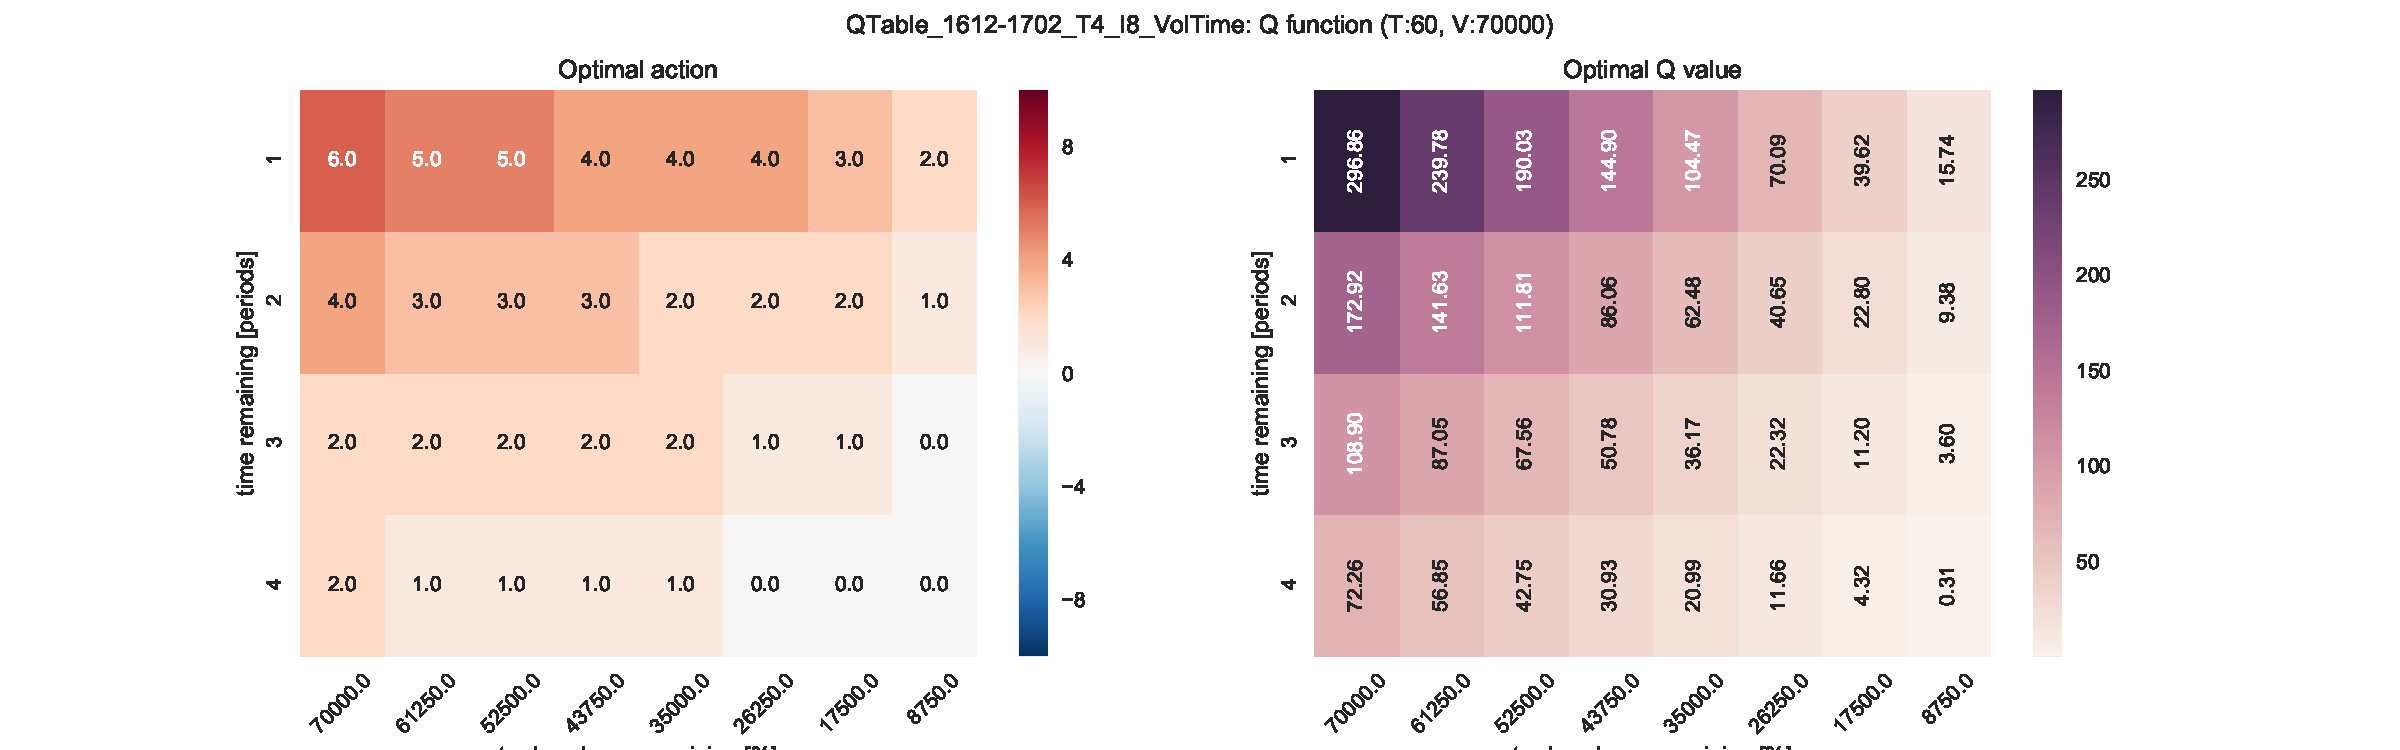
\includegraphics[width=1.\textwidth]{content/drawings/heatmap_3months}
	\caption{Final State-Action function.}
	$T=4$ (60min), $I=8$ (70.000\$), L=15 ([-4, -3, \ldots{}, 9, 10])
	\label{fig:heatmap}
\end{figure}

\Cref{fig:heatmap} illustrates clearly, how the optimal strategy becomes more aggressive as time ceases and a large portion of the trading volume remains unexecuted.
\vspace{0cm}

\section{Forward learning}
\label{chap:forwardlearning}
In order to collect more realistic transition samples (see subsequent discussion in \Cref{chap:backwardalgorithm:discussion:markovianassumption}), an alternative, \emph{forward sampling} method is presented.

\subsection{Forward Sampling \& Learning}
Rather than examining all available actions on the great variety of combinational possibilities the state space has to offer, the forward approach repeatedly simulates trades in their entirety. The once again utilized \ac{OTS} always starts with $V=100\%$, but may be initialized at random start points (\eg \lstinline!t=0, t=15, t=30, t=45!) and keeps going until the full trade is executed.\\

As such, the obtained transitions stem from a more natural and furthermore fully continuous environment. Only actually attainable states, that could arise in the (simulated) reality, are used as transition start points, potentially increasing their significance. As major disadvantage, this forward sampling approach does not assure exhaustive exploration of the state space. A thorough exploration is not self-evident and must be supervised.\\

The pseudo-code of the forward sampling approach is shown in \Cref{alg:forward:pseudocode}. The algorithm iterates over the training data, starts $E$ exploration phases per orderbook window and follows an $\epsilon$-greedy exploration strategy. Each exploration phase starts with $\epsilon=1.0$ which finally decays to $\epsilon=0.05$ according to $\epsilon=0.05^{e/E}$.\\

If $\epsilon$-greedy proposes an actions, that previously led to an end state (\ie trade completed), an alternative action is sampled according to a gaussian distribution with its peak at the originally proposed action. Before the actual random draw, probabilities of all dead-end-actions are set to zero, to forestall pointless resampling. In case of repeatedly running into dead-ends (\eg \lstinline!max_dead_ends=4!) the exploration phase is aborted and continues with the next orderbook.\\

After every \lstinline!retrain! exploration phases, the new samples are fit into the agents model (\eg \lstinline!retrain=256!) and the updated model used for future $\epsilon$-greedy exploration. Prior to the sampling phase, the training set is shuffled.\\

In contrast to the backward sampling method, market variables may be queried on the go, such that they entail the strategies impact. Because sample trajectories stem from a continuous state space function approximations prove handy. Here a RandomForestRegressor (\ie \ac{BT}) is utilized and retrained from scratch every \lstinline!retrain! exploration phases. The alternative approach of exploiting Neural Fitted Q-iteration \Cite{Riedmiller:2005:NFQ}, has been  postphoned to future experiments.\\

\begin{algorithm}[H] 
 \caption{Forward sampling and learning approach.}
     \SetAlgoLined
     \footnotesize
     
     \KwIn{data, V=$70.000\$$, H=60min, T=4, L=[-4..10], E=60, retrain=256}

Shuffle(data)\;
Split data into chunks of length $retrain$

\While{not end of chunks}{
\For{orderbook window in chunks}{
Init OTS(orderbook\_window, V, H, T, L)\;
    \For{epoch=0 to E}{
        Reset OTS to $V=100\%$ and random time point (in H)\;
        \Repeat{$V=0\%$}{
        Set $x_t=[\text{time\_left}, \text{volume\_left}, o_1, ..., o_R]$\;
        Enquire $\epsilon$-greedy action from model\;
        \If{action chain led to an end state previously}{choose other action}
        Apply action\;
        Remember transition \{$x_t, action, cost, x_{t+1}$\}
        }
    }
    Retrain model from collected transitions (growing batch)
    }
}

\label{alg:forward:pseudocode}
\end{algorithm}\bigskip







\section{Discussion}
\label{chap:backwardalgorithm:discussion}
While the presented backward algorithm exploits the available data profoundly in a brute force manner, the underlying assumptions deserve a short discussion. Alternative formulations are tested out, to potentially improve the algorithms cost saving capabilities.

\subsection{Subject of Trade}
\label{chap:backwardalgorithm:discussion:subjectTrade}
Nevmyvaka \etal \cite{Nevmyvaka:2006} tackled the problem of trading a certain amount of shares within a fixed time period. A more practicable problem definition must distinguish between the concrete trading direction. While their problem definition fits to the case of selling shares that are in the investors possessions, it does not mirror the opposite case properly. If the subject of trade is to obtain shares, it is more realistic to define a fixed amount of disposable \emph{cash}, rather than the number of \emph{shares}, that shall be acquired. Subsequently, all experiments in buy direction are instructed to commute a fixed amount of cash into as many shares as possible.\\
 
If cash is the subject of trade, the optional market variable \emph{Immediate Market Order Cost}  (\eg $72.321\$$) becomes meaningless, and will be replaced by \emph{Immediate Market Order Shares} (\eg 92 BTC), displaying the number of shares acquirable with a immediately.

\subsection{Discrete State Space}
The algorithms most obvious weakness lies in its vulnerability to seldomly observed market situations. Since the state-action function is implemented as a simple lookup table without any generalization capabilities, it is strictly dependent on a thorough exploration of the underlying state space. As exhaustive exploration is enforced for the value range of private variables only, market variables are entrusted to chance. Especially when increasing the state space dimension by adding multiple market variables simultaneously, the explanatory power of a learned state-action mapping depends crucially on the number of underlying observations. There exists even the chance of certain states never been monitored at all during the training phase.\\

The concrete discretization process was not further described or questioned. Particularly it is not stated, how boundaries between 0 (low), 1 (medium) and 2 (high) have been chosen, and how the trading performance may be influenced by a higher market variable resolution.

\begin{description}
\item[Potential Improvements] are described and tested in \Cref{chap:experiments}.\\
Firstly, the discretization is automatized, such that boundaries between bins are automatically derived from the training data. Varying discretization resolutions are tested. Secondly, the underlying lookup tables are replaced by function approximations, making discretization unnecessary.
\item[Alternative Market Variables] may be considered.\\
Except for \emph{Immediate Market Order Cost}, the market variables exploited (see \Cref{chap:statespace}) basically came from market level 1 data only. \Cref{chap:exp:additionalmarketvars} evaluates the impact of additional market level 2 features, describing potential imbalances between ask and bid book and forecasting estimated action consequences.
\end{description}



\subsection{Cost scaling}
\label{chap:backwardalgorithm:discussion:costscaling}
\begin{wrapfigure}{r}{0.35\textwidth}
	\centering
	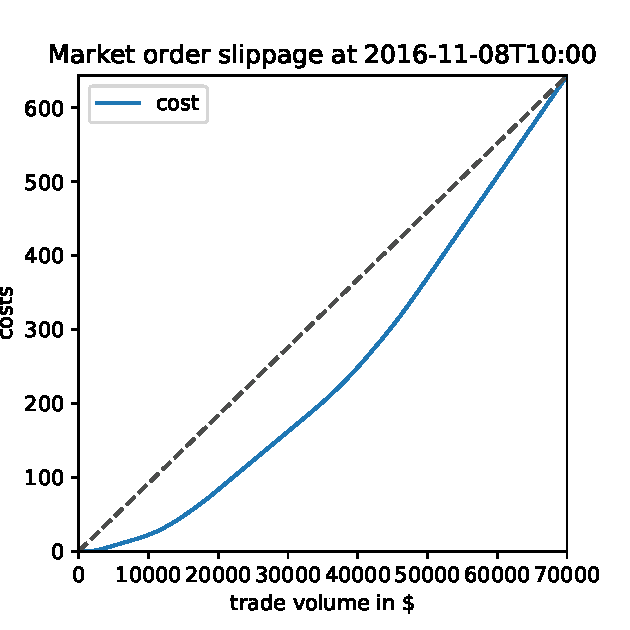
\includegraphics[width=0.3\textwidth,trim={0 0.2cm 0 0.7cm},clip]{content/drawings/nonlinearcosts}
	\caption{Non-linear slippage growth.}
	\label{fig:nonlinearcosts}
\end{wrapfigure}
While discretization of market variables mainly affects the strategies explanatory power, the resolution of private variable \lstinline!volume! leads to considerable rounding issues in regards to the cost function employed. As observed successor states $x_{t-1}$ must be discretized equally to allow looking up the corresponding minimal costs, the immediate costs, as computed in \Cref{eq:imcost}, must be scaled accordingly. Simply replacing \lstinline!volume_traded! with \lstinline!round(volume_traded)! falsifies the actual costs, as they correlate to the accomplished trade volume in an  unpredictable, non-linear manner as indicated in \Cref{fig:nonlinearcosts}. Nevmyvaka \etal \Cite{Nevmyvaka:2006} did not mention this problematic and presumably did not perform any cost scaling at all.

\begin{description}
\item[Potential Improvements]  A simple, but imprecise approach is to perform cost scaling, as described above. In general, this problem should be void, when function approximations are trained from the original float values, instead of rounded values.
\end{description}


\subsection{Markov Property}
\label{chap:backwardalgorithm:discussion:markovianassumption}
The proposed backward algorithm assumes individual \lstinline!trading_periods! to be of an (approximately) Markovian nature. This is in fact not true, as the \ac{OTS}'s internal masterbook shape depends drastically from the preceding trade history.\\

\Cref{fig:differingmasterbooks} shows differing masterbook shapes, that can build the base of a simulated \lstinline!trading_period!, \eg if starting at $t=45min$ and a remaining trade volume of 17.500\$. \ref{fig:differingmasterbooks:NoSim} shows the original orderbook, as if no orders had been matched by our strategy. This version of the masterbook is queried by the original backward algorithm, potentially resulting in more passive trading aggressions, as it does not account for the own impact on the market at all. \ref{fig:differingmasterbooks:SimMarketOrder} and \ref{fig:differingmasterbooks:SimEq} show two ideas, how the market impact can be incorporated. Both lead to different masterbook shapes and to different subsets of attainable prices.\\

\begin{figure}[ht]
	\centering
	\begin{subfigure}[t]{0.3\textwidth}
        		\centering
        		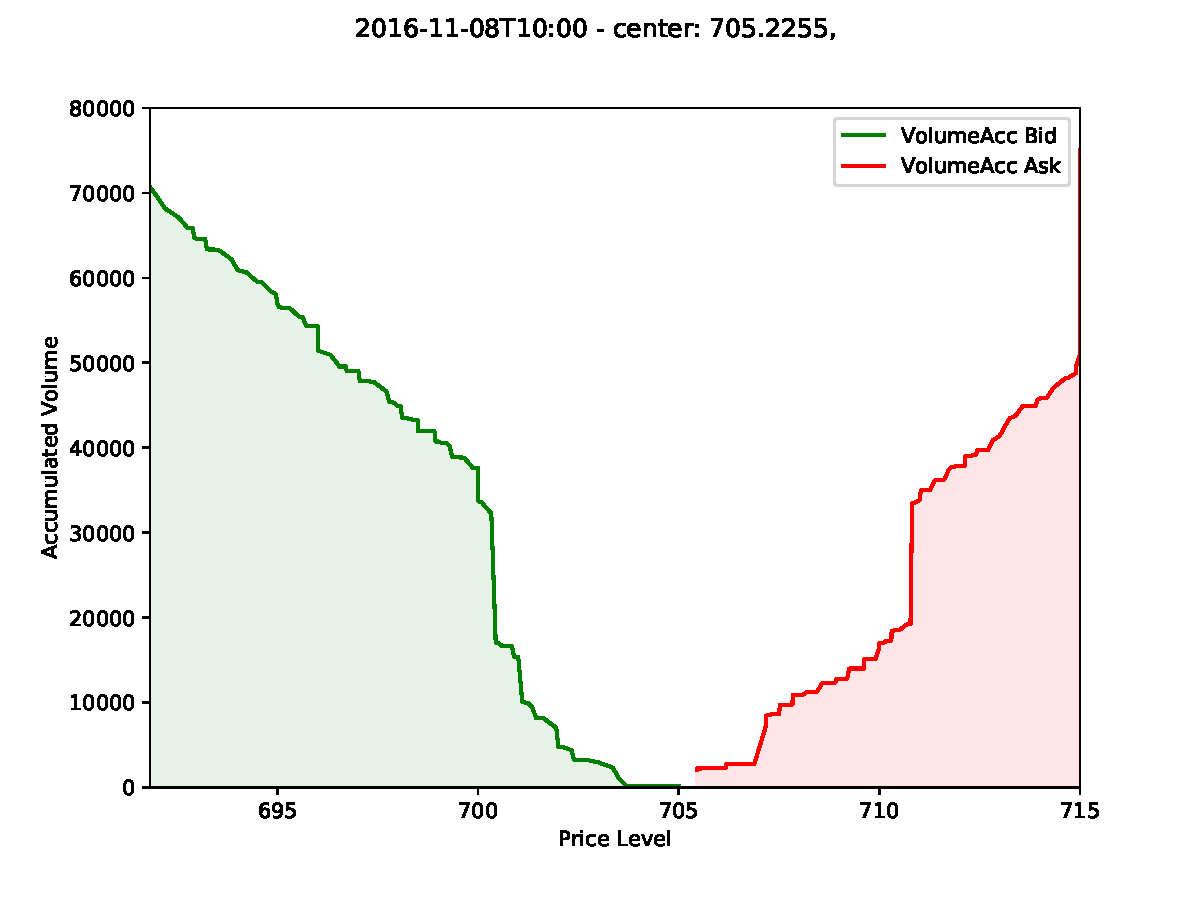
\includegraphics[width=\textwidth]{content/drawings/masterbook_customstart_NoSim}
        		\caption{Original Orderbook.}
		\label{fig:differingmasterbooks:NoSim}
    	\end{subfigure}
	\begin{subfigure}[t]{0.3\textwidth}
        		\centering
        		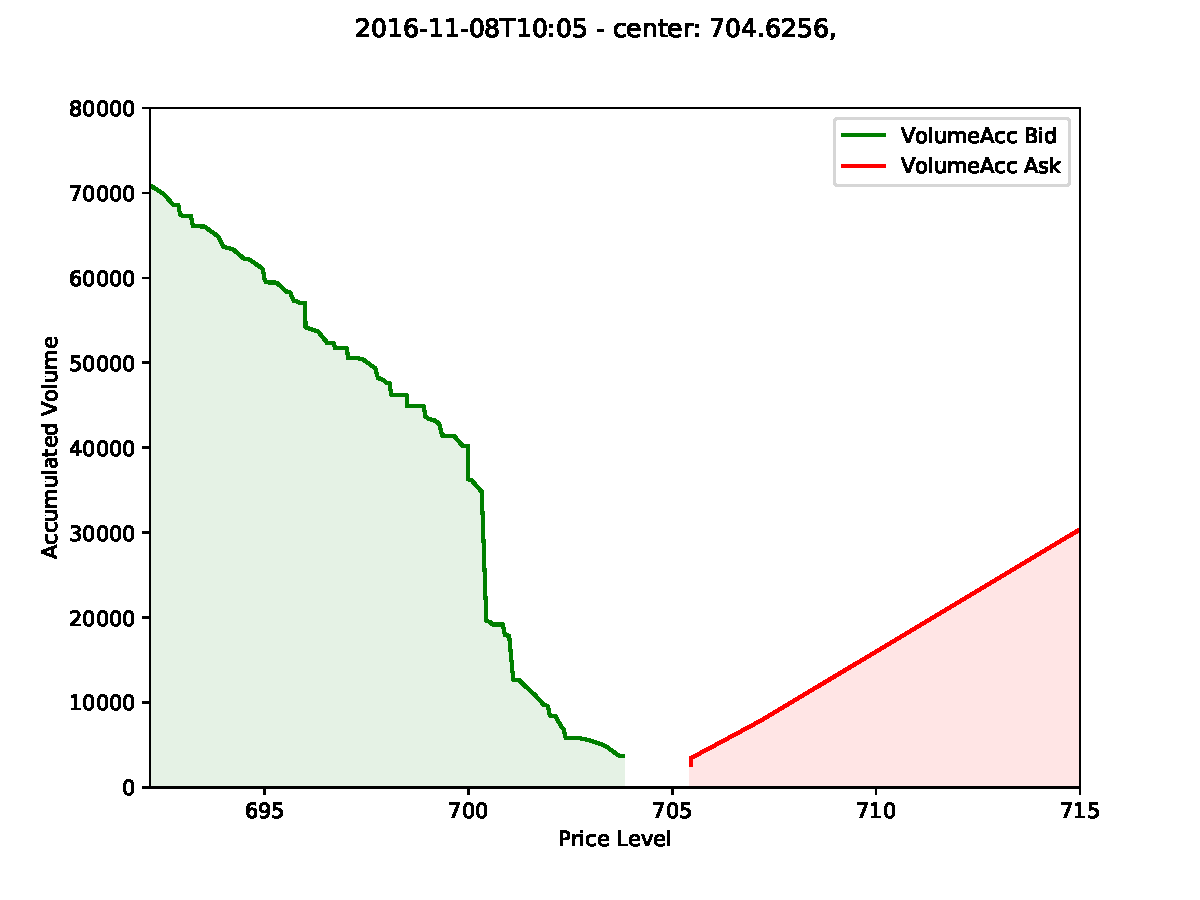
\includegraphics[width=\textwidth]{content/drawings/masterbook_customstart_SimMarketOrder}
        		\caption{Assuming 52.500 shares being matched at \lstinline!t=0!, then no further matches.}
		\label{fig:differingmasterbooks:SimMarketOrder}
    	\end{subfigure}%
	\begin{subfigure}[t]{0.3\textwidth}
        		\centering
        		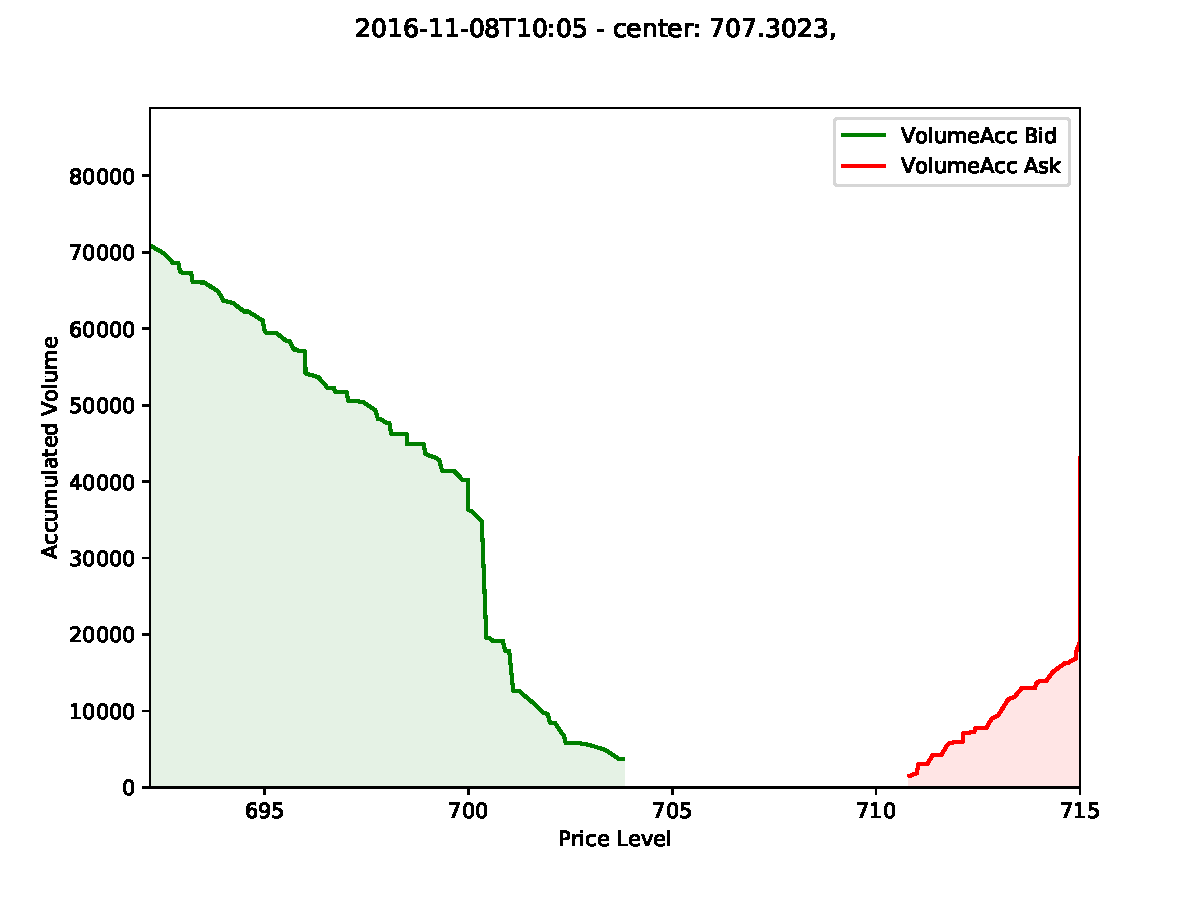
\includegraphics[width=\textwidth]{content/drawings/masterbook_customstart_SimEqual}
        		\caption{Assuming 52.500 shares being matched evenly at 1.166 shares per minute.}
		\label{fig:differingmasterbooks:SimEq}
    	\end{subfigure}%

	\caption{Different shaped masterbooks at \lstinline!t=45!.}
	The shapes differ, depending on the preceding trade history.
	\label{fig:differingmasterbooks}
\end{figure}

\begin{description}
\item[Potential Improvements] Initializing the \ac{OTS} outside the original start point ($t=0, V=100\%$), the supposedly traded volume must be incorporated, \eg as done in \Cref{fig:differingmasterbooks:SimEq}. Other than that, a more realistic sampling method may be applied: The forward sampling process, described in \Cref{chap:forwardlearning}, approaches sampling from the other side. Rather than evaluating actions on individual \lstinline!trading_periods!, the \ac{OTS} always starts with $V=100 \% $ and keeps going until the full trade is executed. As such, more realistic samples are generated. This does not give the problem a Markovian nature, but the internal masterbook is always of a realistic shape. In contrast to the backward approach, exhaustive exploration of the state space is not self-evident and must be enforced.
As a side benefit, the forward sampling approach generates more versatile samples for training the function approximates, as the generated samples do not necessarily start at \emph{discrete} start points only.
\end{description}



\subsection{Action Space}
\label{chap:backwardalgorithm:discussion:actionspace}
The mapping from actions to limits deserves some reflection as well. The proposed method (see \Cref{chap:actionspace}) adds the value of the chosen action directly to the current best price of the opposing book, such that the bid-ask spread must be crossed before any orders may be matched.\\

On the one hand, it seems pointless to fix the origin at the best price of the \emph{opposing} book. By doing so, it appears obvious, that decisions derived from state spaces including a variable for the current spread size, outperform decisions derived from state spaces not including this market variable. Indeed, the  bid-ask spread was posed as the market variable causing the greatest individual impact on cost reduction, namely -$7.97\%$, which is a major fraction of the maximum achievement of  $-12.85\%$\footnote{Strategies derived from five dimensional state spaces including the market variables Spread, ImmCost \& Signed Vol, as described in \Cref{chap:costs}, outperformed strategies derived from two dimensional state spaces, containing the private variables only, by $-12.85\%$ in average.}.\\

On the other hand, the proposed mapping method does not necessarily fit to the Bitcoin data at hand. As is shown in \Cref{fig:ploniexPriceHistory}, Bitcoin prices have burst from roughly 700\$ to more than 2.000\$ in the period of recording, \ie interpreting actions as the absolute difference to the current best prices, maps to significantly different levels of aggression as time passes.


\begin{description}
\item[Potential Improvements] lay in alternative action-limit mappings.\\
On the one hand side, the limit base may be fixed to the other side of the bid-ask-spread, reducing pointless dependencies on the speads size. On the other hand, actions should be interpreted as factors, rather than summands to allow for a consistent aggression interpretation. 
The mapping functions are thus redefined as follows:\\
\lstinline!limit_buy = ask * (1 + (a/1000))! instead of \lstinline!limit_buy = bid + a!\\
\lstinline!limit_sell = bid * (1 - (a/1000))! instead of \lstinline!limit_sell = ask - a!.

Actions $a$ now represent the deviation from the limit base in per mile. The influence of the chosen limit base is analyzed in \Cref{chap:exp:actionlimitmapping}.
\end{description}


\cleardoublepage{}
\chapter{Discussion and Experiments}
\label{chap:orderbookagents}
This chapter summarizes various experiments, that have been conducted to examine the agents ability to find optimal solutions to the problem of optimized trade execution. The recorded orderbook snapshots for currency pair USDT/BTC (see \Cref{chap:dataorigin}) have been split into training period (Nov, 10th 2016 - Apr, 30th 2017) and test period (May 2017).\\

All experiments refer to the very same environment settings and build up on each other to some extend. The agents common task is to buy Bitcoins worth of 70.000\$ within a trading horizon of 60 minutes. The problem definition is opposed to the task evaluated by Nevmyvaka \etal \cite{Nevmyvaka:2006}, where the number of shares (respectively Bitcoins) is fixed, rather than the amount of cash.\\

The training set translates into 4.154 orderbook windows, while the test set gives 724 orderbook windows. A period length of 15 minutes is assumed, such that the \ac{OTS} expects up to $T=4$ order limit prices. Private variable \lstinline!volume! is discretized in 8 intervals, \ie $I=[8.750\$,..,70.000\$]$, and the action space consists of fifteen actions $L=[-4, -3, ..., 8, 9, 10]$. In line with the formulas presented in \Cref{chap:actionspace}, these actions translate into order limits deviating by $-0.4\%$ to $+1.0\%$ from the current best price.


\subsection{Baseline}
\label{chap:experiments:baseline}
Simple \ac{SL} strategies (see \Cref{chap:tradingstrategies}) and immediate market order placements serve as benchmark for the performance measurement.\\

\begin{figure}[ht]
	\centering
	\begin{subfigure}[b]{0.5\textwidth}
        		\centering
        		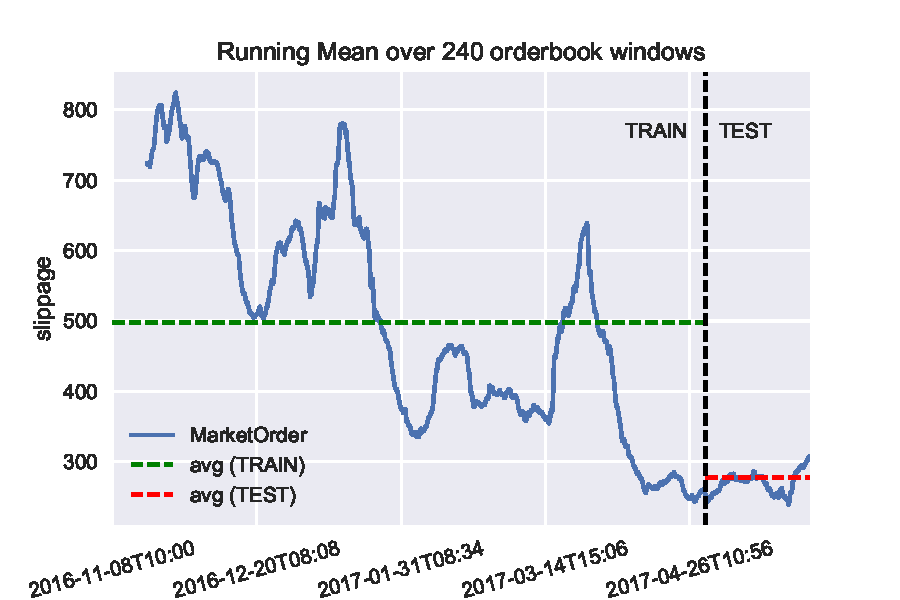
\includegraphics[width=\textwidth]{content/drawings/runningMean240_MarketPrice}
        		\caption{Observed Market Order Slippage.}
		\label{fig:runningmean:marketPrice}
    	\end{subfigure}%
	\begin{subfigure}[b]{0.5\textwidth}
        		\centering
        		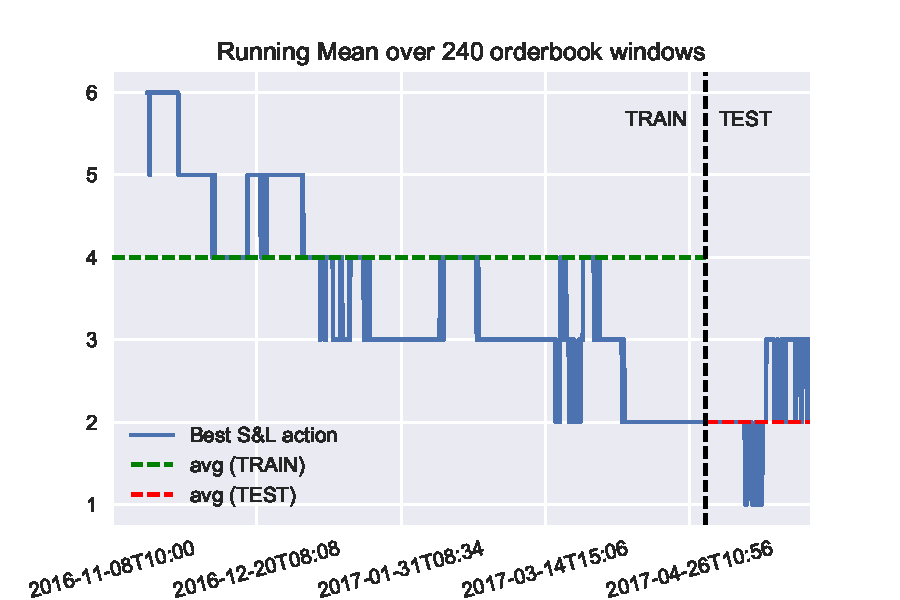
\includegraphics[width=\textwidth]{content/drawings/runningMean240_bestAction}
        		\caption{Best S\&L action.}
		\label{fig:runningmean:bestaction}
    	\end{subfigure}

	\caption{Concurrent to declining slippage, the optimal \ac{SL} actions become less aggressive as time passes.}
	\label{fig:runningmean}
\end{figure}


\begin{figure}[ht]
        	\centering
        	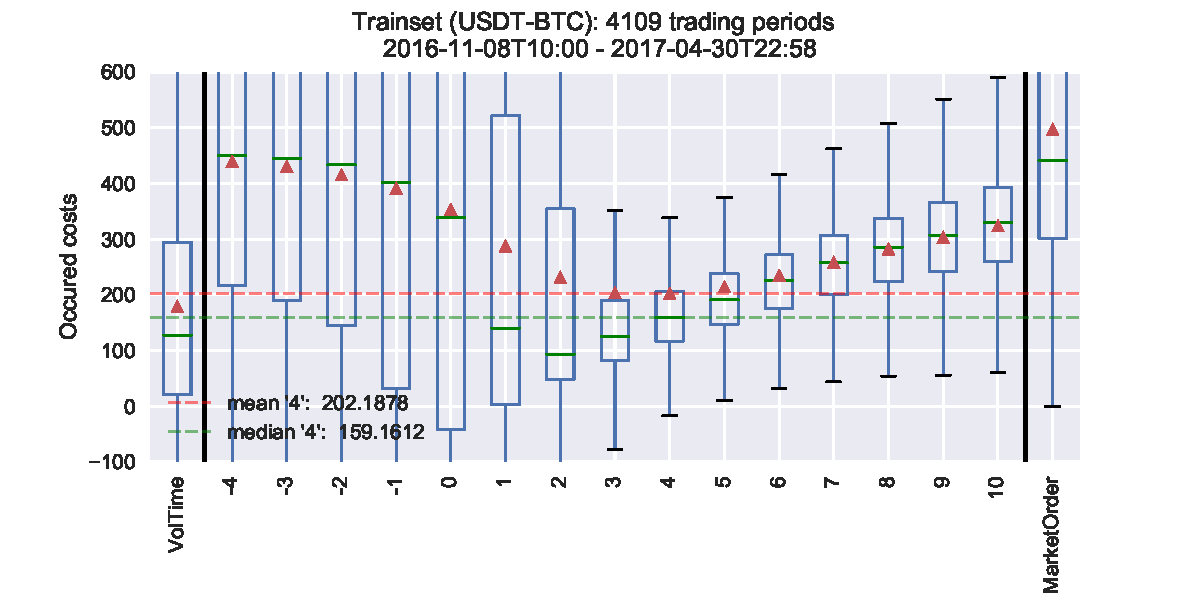
\includegraphics[width=\textwidth]{content/drawings/bestActionTrain}
	\caption{Average costs induced by the varying \ac{SL} actions over the full training period. In average, action 4 performed best.}
	\label{fig:bestAction}
\end{figure}

Due to bursting Bitcoin prices (see \Cref{chap:dataorigin}, \Cref{fig:ploniexPriceHistory}), the investigated sum of 70.000\$ constitutes a declining contingent of the total market volume. \Cref{fig:runningmean:marketPrice} shows a running average over the amount of slippage, as induced by immediate market orders. Concurrent to declining slippage, the optimal \ac{SL} actions become less aggressive as time passes. The green, dashed lines show the respective average over the training period, which significantly differs from the red, dotted line referring to the average over the test period. \Cref{fig:bestAction} shows the average costs, induced by varying \ac{SL} strategies within the training period.\\

In order to provide a more realistic and unexaggerated baseline, the optimal \ac{SL} action is estimated from the test period. As such, performances of subsequents experiments are compared to the performance of a simple market order and the \ac{SL} strategy "2", with the initial order limit fixed to 1.002 times the initial ask (\ie $+0.2\%$).


\section{Examined Issues}
\label{chap:backwardalgorithm:discussion}
While the presented backward algorithm exploits the available data profoundly in a brute force manner, the underlying assumptions deserve a short discussion. Alternative formulations are tested out, to potentially improve the algorithms cost saving capabilities.

\subsection{Action-Limit Mapping}
\label{chap:backwardalgorithm:discussion:actionspace}
By fixing the limit base at the best price of the \emph{opposing} book, it appears obvious, that decisions derived from state spaces including a variable for the current spread size, outperform decisions derived from state spaces not including this market variable. Indeed, in the original paper\Cite{Nevmyvaka:2006} the bid-ask spread was posed as the market variable causing the greatest individual impact on cost reduction, namely -$7.97\%$, which is a major fraction of the maximum achievement of  $-12.85\%$\footnote{Strategies derived from five dimensional state spaces including the market variables Spread, ImmCost \& Signed Vol, as described in \Cref{chap:costs}, outperformed strategies derived from two dimensional state spaces, containing the private variables only, by $-12.85\%$ in average.\Cite{Nevmyvaka:2006}}.\\

The positive impact of moving the limit base to the opposite book, as proposed in \Cref{chap:actionspace}, is shown in \Cref{chap:exp:actionlimitmapping}.


\subsection{Discrete State Space}
The most obvious weakness of the discrete backward approach lies in its vulnerability to seldomly observed market situations. Since the state-action function is implemented as a simple lookup table without any generalization capabilities, it is strictly dependent on a thorough exploration of the underlying state space. As exhaustive exploration is enforced for the value range of private variables only, market variables are entrusted to chance. Especially when increasing the state space dimension by adding multiple market variables simultaneously, the explanatory power of a learned state-action mapping depends crucially on the number of underlying observations. There exists even the chance of certain states never been monitored at all during the training phase.\\

Consequently, the impact of different market variables at varying levels of discretization is examined, starting in \Cref{chap:exp:additionalmarketvars}. Eventually, the effect of replacing the underlying lookup table with function approximators is studied in \Cref{chap:experiment:functionApprox}. 





\subsection{Markov Property}
\label{chap:backwardalgorithm:discussion:markovianassumption}
The proposed backward algorithm (see \Cref{chap:backwardlearning}, \Cref{alg:bruteforce:pseudocode}) assumes individual \lstinline!trading_periods! to be of an (approximately) Markovian nature. As explained in \Cref{chap:backwardapproach:precedingTrades}, the \ac{OTS}'s internal masterbook shape depends drastically from the preceding trade history. Since all relevant information from the history must be taken into account, two approaches are examined, that aim to generate more realistic samples and as such to strengthen the Markov Property of states:\\

The advantage of the improved backward algorithm, that incorporates preceding trades prior to actual trade simulations (see \Cref{chap:backwardapproach:precedingTrades}, \Cref{alg:bruteforceimproved:pseudocode}), is shown in \Cref{chap:exp:simulatedTrades}. \Cref{chap:experiments:forward} demonstrates, that the novel forward sampling algorithm described in \Cref{chap:forwardlearning} outperforms all other methods, as strategies are derived from a more realistic set of sample transitions.

% than that, a more realistic sampling method may be applied: The forward sampling process, described in \Cref{chap:forwardlearning}, approaches sampling from the other side. Rather than evaluating actions on individual \lstinline!trading_periods!, the \ac{OTS} always starts with $V=100 \% $ and keeps going until the full trade is executed. As such, more realistic samples are generated. This does not give the problem a Markovian nature, but the internal masterbook is always of a realistic shape. In contrast to the backward approach, exhaustive exploration of the state space is not self-evident and must be enforced.
%As a side benefit, the forward sampling approach generates more versatile samples for training the function approximates, as the generated samples do not necessarily start at \emph{discrete} start points only.







\section{Backward Learning}
\label{chap:experiments}
In the following, backward learning experiments that paved the way towards improved trade execution strategies are presented.

\subsection{Action-Limit Mapping}
\label{chap:exp:actionlimitmapping}
As mentioned in \Cref{chap:backwardalgorithm:discussion:actionspace}, it seems pointless to force actions to cross the bid-ask-spread before any orders can be matched. \Cref{fig:actionlimitmapping} shows exemplary for November 2016, how the choice of the limit base affects the agents trading performance.\\

\begin{table}[ht]
	\centering
		\scalebox{0.7}{
\rowcolors{1}{}{black!5}
\begin{tabular}{|lRR|}
\toprule
{} &           slippage & performance \\
\midrule
currBid         	     &  220.19 & 92.6\%\\
currBid\_mSpread &  218.71 & 91.9\%\\
currBid\_spread     &  215.76 & 90.7\%\\
\midrule
currAsk                  &  214.00 & 90.0\%\\
currAsk\_mSpread &  214.53 &90.2\%\\
currAsk\_spread    &  215.38 & 90.6\%\\
\midrule
S\&L: 5         	      & 237.75 & 100.0\%\\
MarketOrder          & 737.58 & 310.2\%\\
\bottomrule
\end{tabular}	
		} 
	\caption{Evaluating the impact of different limit base levels.}
	\small Results stem from applying the respective strategies on all 537 orderbook\\ windows recorded between Nov, 10th 2016 and Nov, 30th 2016.
	\label{fig:actionlimitmapping}
\end{table}

While buy orders, forcing agents to cross the bid-ask-spread (\ie \lstinline!currBid*!), typically benefit from the two market variables \lstinline!spread! and \lstinline!marketSpread!, this is not necessarily the case for agents which have the limit base fixed to the opposing best price (\ie \lstinline!currAsk*!). As the latter agents consistently showed better performance, the limit base is henceforth fixed to the best price of the corresponding trading direction.





\subsection{Additional Market Variables}
\label{chap:exp:additionalmarketvars}
In addition to the originally proposed market variables (see \Cref{chap:statespace}), the following orderbook features have been examined:

\begin{description}
\item[marketPrice*] describes the relative difference between current center price and the worst price that must be paid (or is received) in case of simple market orders.

\item[sharecount\_*] quotes the number of Bitcoins, immediately available for $70.000\$$.\\
\lstinline!sharecount_buy! is tantamount to the originally proposed \lstinline!ImmCost! (See \Cref{chap:backwardalgorithm:discussion:subjectTrade}).

\item[center\_price] was added as a consequence of the findings from \Cref{chap:experiments:baseline}, \Cref{fig:runningmean}: Apparently, as the ratio between current Bitcoin price and the investable $70.000\$$ increases, an optimal strategy may have to place less aggressive order limits.

\item[\_a*\_effects] quotes the minimum volume immediately obtainable by individual actions. The value is a lower bound of the truly obtainable volume, because only the current orderbook is retrievable. New opportunities, arising within the forthcoming \lstinline!trading_period! are unacquainted and not included.
\end{description}


 \Cref{tab:eval:additionalMarketVariables} shows the performance of individual QTable agents trained on both private variables plus one discretized market variable attached at a time. While observed trading costs undercut those induced by simple market orders by $-49.16\%$, the gain in comparison to the optimal \ac{SL} strategy lies at $-8.93\%$.\\
 
Adding the market variable \lstinline!spread! yields a notable improvement of $-4.84\%$ over the plain \lstinline!VolTime!-agent. By increasing the discretization level to 5, the performance can be further improved to $-6.34\%$, verifying the findings of Nevmyvaka�\etal \Cite{Nevmyvaka:2006}. However, in contrast to their reported results, the market variable \lstinline!sharecount_buy! falls flat with a worsening of $+6.70\%$ (compared to $-4.26\%$).\\
 
Disappointing is the futility of \lstinline!center_price!. For a discretization level of 5, the corresponding agent underperforms the plain \lstinline!VolTime!-agent by $+7.35\%$. Potentially, this may be explained by a compulsorily underexploited training set: Due to generally rising Bitcoin prices, the majority of prices in the test period will map to the highest discretization value available, which, in a simple lookup-table, resembles only a fraction of the assessed training set.\\

\begin{table}[ht]
	\centering
	\scalebox{0.6}{
	\rowcolors{1}{}{black!5}
\begin{tabular}{|lRRR|RRRR|}
\toprule
{} &  \text{slippage} &     \text{med} &     \text{std} &   \text{perf\_2} &   \text{perf\_4} &   \text{perf\_M} & \text{perf\_VolTime} \\
\midrule
center\_price\_disc3            &    149.57 &   46.15 &  420.14 &   -3.44\% &  -15.19\% &  -46.10\% &       -0.70\% \\
center\_price\_disc5            &    161.70 &   37.83 &  450.36 &    +4.39\% &   -8.32\% &  -41.73\% &        \cellcolor{red!25}+7.35\% \\
marketPrice\_buy\_worst\_disc5  &    146.83 &   39.62 &  351.77 &   -5.21\% &  -16.75\% &  -47.08\% &       -2.52\% \\
marketPrice\_sell\_worst\_disc5 &    148.94 &   42.71 &  388.86 &   -3.85\% &  -15.55\% &  -46.33\% &       -1.12\% \\
marketPrice\_spread\_disc5     &    150.46 &   44.15 &  371.32 &   -2.87\% &  -14.69\% &  -45.78\% &       -0.11\% \\
marketPrice\_imbalance\_disc5      &    150.10 &   68.68 &  336.60 &   -3.10\% &  -14.90\% &  -45.91\% &       -0.35\% \\
sharecount\_buy\_disc3         &    149.57 &   46.15 &  420.14 &   -3.44\% &  -15.19\% &  -46.10\% &       -0.70\% \\
sharecount\_buy\_disc5         &    160.73 &   37.78 &  449.22 &    +3.76\% &   -8.87\% &  -42.08\% &        \cellcolor{red!25}+6.70\% \\
sharecount\_imbalance\_disc5   &    148.03 &   40.49 &  372.86 &   -4.44\% &  -16.07\% &  -46.65\% &       -1.73\% \\
sharecount\_sell\_disc5        &    151.50 &   47.49 &  425.35 &   -2.20\% &  -14.10\% &  -45.40\% &        +0.58\% \\
sharecount\_spread\_disc5      &    148.93 &   40.84 &  352.12 &   -3.86\% &  -15.56\% &  -46.33\% &       -1.13\% \\
spread\_disc3                 &    147.41 &   35.48 &  370.96 &   \cellcolor{black!20}-4.84\% &  -16.42\% &  -46.88\% &       -2.14\% \\
spread\_disc5                 &    \cellcolor{green!25}141.07 &   \cellcolor{green!25}37.39 &  \cellcolor{green!25}349.72 &   \cellcolor{green!25}-8.93\% &  \cellcolor{green!25}-20.02\% &  \cellcolor{green!25}-49.16\% &       \cellcolor{green!25}-6.34\% \\
spread\_disc9                 &    142.80 &   36.69 &  364.76 &   -7.81\% &  -19.03\% &  -48.54\% &       -5.20\% \\
\midrule
VolTime                      &    150.63 &   33.83 &  358.66 &   -2.76\% &  -14.60\% &  -45.72\% &        0.00\% \\
2                            &    154.90 &   68.62 &  389.15 &    0.00\% &  -12.17\% &  -44.18\% &        +2.84\% \\
4                            &    176.37 &  141.66 &  273.58 &   +13.86\% &    0.00\% &  -36.44\% &       +17.09\% \\
MarketOrder                  &    277.49 &  246.48 &  158.66 &   +79.14\% &   +57.33\% &    0.00\% &       +84.22\% \\
\bottomrule
\end{tabular}
	}  		 
        		\caption{Evaluating the impact of additional market variables.}
		\small Average performance over the test period may 2017, currency pair USDT/BTC.\\
		See \Cref{appendix:additionalMarketVariables}, \Cref{tab:eval:additionalMarketVariables:fulltable} for complete results.
		\label{tab:eval:additionalMarketVariables}

\end{table}

The different discretization levels yield rather mixed results. While \lstinline!spread! typically performed best in case of 5 levels, no clear statement can be made for the other variables.\\

The exact reason, why factually only adding \lstinline!spread! causes a beneficial effect, is unclear, but one possible explanations lies in the data set employed. The original experiment assessed a different data quality. Due to the low resolution of the available orderbook snapshots, a large fraction of the market activity remains inaccessible and consequently the majority of trading opportunities are missed by the agents. Furthermore, the minute time-scaled data inevitably requires the trading horizon to be rather long. Experiments with shorter time horizons nullified the achievable savings, while longer time horizons led to unacceptable computation times. Consequently, the agents where trained on $4.109$ sixty-minute orderbook windows, while Nevmyvaka \etal invoked $45.000$ two-minute orderbook windows.


\subsection*{Look-Ahead Features}
\label{chap:experiments:lookahead}
In order to proof the algorithms general ability to find costs reducing strategies, look-ahead features\footnote{look-ahead features provide a glance into the future, and are thus equivalent to cheating.} were added to the universe of market variables. \lstinline!future_center*! quotes percentual changes between the current center price and the center price in 5, 15 and 60 minutes respectively. This hypothetical knowledge about future price trends reduces observed trading costs by $-12.47\%$ (\ie $-14.88\%$ over simple \ac{SL} strategy).\\

\begin{table}[ht]
	\centering
	\scalebox{0.6}{
	\rowcolors{1}{}{black!5}
\begin{tabular}{|lRRR|RRRR|}
\toprule
{} &  \text{slippage} &     \text{med} &     \text{std} &   \text{perf\_2} &   \text{perf\_4} &   \text{perf\_M} & \text{perf\_VolTime} \\
\midrule
ob\_direction\_disc5           &     61.99 &   97.52 &  319.84 &  \cellcolor{black!20}-59.98\% &  -64.85\% &  -77.66\% &      \cellcolor{black!20}-58.84\% \\
future\_center5\_disc5         &    141.61 &   41.79 &  389.58 &   -8.58\% &  -19.71\% &  -48.97\% &       -5.98\% \\
future\_center15\_disc5        &    133.78 &   40.90 &  405.88 &  -13.63\% &  -24.15\% &  -51.79\% &      -11.18\% \\
future\_center60\_disc5        &    131.85 &   47.63 &  391.46 &  \cellcolor{green!25}-14.88\% &  -25.25\% &  -52.49\% &      \cellcolor{green!25}-12.47\% \\
\midrule
VolTime                      &    150.63 &   33.83 &  358.66 &   -2.76\% &  -14.60\% &  -45.72\% &        0.00\% \\
2                            &    154.90 &   68.62 &  389.15 &    0.00\% &  -12.17\% &  -44.18\% &        +2.84\% \\
4                            &    176.37 &  141.66 &  273.58 &   +13.86\% &    0.00\% &  -36.44\% &       +17.09\% \\
MarketOrder                  &    277.49 &  246.48 &  158.66 &   +79.14\% &   +57.33\% &    0.00\% &       +84.22\% \\
\bottomrule
\end{tabular}
	}  		 
        		\caption{Evaluating the impact of look-ahead features.}
		\small Average performance over the test period may 2017, currency pair USDT/BTC.\\
		\label{tab:eval:additionalMarketVariables:lookahead}

\end{table}

A vastly larger impact ($-58.84\%$ respectively $-59.98\%$) is caused by the look-ahead feature \lstinline!ob_direction!, quoting the general price trend of the currently observed orderbook window. In contrast to the \lstinline!future_center*! variables, it's value stays constant within individual orderbook windows: \lstinline!ob_direction = orderbook[-1].get_center() / orderbook[0].get_center()!, which seems to provoke more stable strategies.


\subsection*{Constant Market Variables}
\label{chap:exp:additionalmarketvars:constant}
The findings from the look-ahead features encouraged for a supplementary experiment. Rather than considering the actual market situation, the market variables are observed once (at \lstinline!t=0!), and kept frozen for the remaining trading horizon. Hope was, to provoke more stable strategies, as the agents could potentially decide on a \emph{major} strategy and consequently only adapt the limits to the private variables representing the actual trade progress.\\

\begin{table}[ht]
	\centering
	\scalebox{0.6}{
	\rowcolors{1}{}{black!5}
\begin{tabular}{|lRRR|RRRR|}
\toprule
{} &  \text{slippage} &     \text{med} &     \text{std} &   \text{perf\_2} &   \text{perf\_4} &   \text{perf\_M} & \text{perf\_VolTime} \\
\midrule
center\_orig\_disc3            &    158.96 &   48.93 &  431.17 &    2.62\% &   -9.87\% &  -42.71\% &        +5.54\% \\
center\_orig\_disc5            &    150.37 &   47.01 &  422.14 &   -2.92\% &  -14.74\% &  -45.81\% &       \cellcolor{red!25}-0.17\% \\
marketPrice\_buy\_worst\_disc5  &    150.74 &   50.15 &  402.13 &   -2.69\% &  -14.54\% &  -45.68\% &        +0.07\% \\
marketPrice\_sell\_worst\_disc5 &    157.56 &   43.95 &  379.33 &    +1.72\% &  -10.66\% &  -43.22\% &        +4.61\% \\
marketPrice\_spread\_disc5     &    152.19 &   53.07 &  398.10 &   -1.75\% &  -13.71\% &  -45.15\% &        +1.04\% \\
marketPrice\_imbalance\_disc5      &    147.16 &   47.03 &  383.19 &   -5.00\% &  -16.57\% &  -46.97\% &       \cellcolor{black!20}-2.30\% \\
sharecount\_buy\_disc3         &    149.57 &   46.15 &  420.14 &   -3.44\% &  -15.19\% &  -46.10\% &       -0.70\% \\
sharecount\_buy\_disc5         &    150.37 &   47.01 &  422.14 &   -2.92\% &  -14.74\% &  -45.81\% &       \cellcolor{red!25}-0.17\% \\
sharecount\_imbalance\_disc5   &    152.44 &   53.41 &  400.89 &   -1.59\% &  -13.57\% &  -45.06\% &        +1.20\% \\
sharecount\_sell\_disc5        &    150.37 &   47.01 &  422.14 &   -2.92\% &  -14.74\% &  -45.81\% &       -0.17\% \\
sharecount\_spread\_disc5      &    149.23 &   53.41 &  402.65 &   -3.66\% &  -15.39\% &  -46.22\% &       -0.93\% \\
spread\_disc3                 &    148.92 &   41.70 &  361.12 &   -3.86\% &  -15.57\% &  -46.33\% &       -1.14\% \\
spread\_disc5                 &    \cellcolor{green!25}143.56 &   \cellcolor{green!25}40.78 &  \cellcolor{green!25}350.74 &   \cellcolor{green!25}-7.32\% &  \cellcolor{green!25}-18.60\% &  \cellcolor{green!25}-48.26\% &       \cellcolor{green!25}-4.69\% \\
spread\_disc9                 &    145.54 &   43.25 &  352.05 &   -6.04\% &  -17.48\% &  -47.55\% &       -3.38\% \\
\midrule
VolTime                      &    150.63 &   33.83 &  358.66 &   -2.76\% &  -14.60\% &  -45.72\% &        0.00\% \\
2                            &    154.90 &   68.62 &  389.15 &    0.00\% &  -12.17\% &  -44.18\% &        +2.84\% \\
4                            &    176.37 &  141.66 &  273.58 &   +13.86\% &    0.00\% &  -36.44\% &       +17.09\% \\
MarketOrder                  &    277.49 &  246.48 &  158.66 &   +79.14\% &   +57.33\% &    0.00\% &       +84.22\% \\
\bottomrule
\end{tabular}
	}  		 
        		\caption{Evaluating the impact of constant market variables.}
		\small Average performance over the test period may 2017, currency pair USDT/BTC.\\
		See \Cref{appendix:fixedMarketVars}, \Cref{tab:eval:additionalMarketVariables:fixed:fulltable} for complete results.
		\label{tab:eval:additionalMarketVariables:fixed}

\end{table}

While \Cref{tab:eval:additionalMarketVariables:fixed} shows improved performance for previous bad performers, the leading \lstinline!VolTimeSpread!-agent dropped from $-8.93\%$ to $-7.32\%$. Contrary to initial hopes, this approach did not lead to superior performance and was not further pursued.\\

\subsection{Simulation of preceding trades}
\label{chap:exp:simulatedTrades}
As described in \Cref{chap:backwardalgorithm:discussion:markovianassumption}, the \ac{OTS}'s internal masterbook shape depends drastically from the preceding trade history. In the following, the effect of incorporating the own impact on the market is investigated.\\

\begin{table}[ht]
	\centering
	\scalebox{0.6}{
	\rowcolors{1}{}{black!5}
\begin{tabular}{|lRRR|RRRRR}
\toprule
{} &  \text{slippage} &     \text{med} &     \text{std} &   \text{perf\_2} &   \text{perf\_4} &   \text{perf\_M} & \text{perf\_VolTime} \\
\midrule
center\_orig\_disc3              &    158.97 &   48.93 &  431.16 &    +2.62\% &   -9.87\% &  -42.71\% &        +5.54\% \\
center\_orig\_disc5              &    150.47 &   47.49 &  422.12 &   -2.86\% &  -14.69\% &  -45.78\% &       -0.11\% \\
marketPrice\_buy\_worst\_disc5    &    148.33 &   47.46 &  400.73 &   -4.24\% &  -15.90\% &  -46.55\% &       -1.53\% \\
marketPrice\_sell\_worst\_disc5   &    154.06 &   42.10 &  370.91 &   -0.54\% &  -12.65\% &  -44.48\% &        +2.28\% \\
marketPrice\_spread\_disc5       &    151.12 &   53.07 &  395.68 &   -2.44\% &  -14.32\% &  -45.54\% &        +0.33\% \\
marketPrice\_imbalance\_disc5        &    143.86 &   47.05 &  375.43 &   -7.13\% &  -18.44\% &  -48.16\% &       -4.49\% \\
sharecount\_buy\_disc3           &    149.57 &   46.15 &  420.14 &   -3.44\% &  -15.19\% &  -46.10\% &       -0.70\% \\
sharecount\_buy\_disc5           &    150.47 &   47.49 &  422.12 &   -2.86\% &  -14.69\% &  -45.78\% &       -0.11\% \\
sharecount\_imbalance\_disc5     &    151.92 &   53.41 &  400.69 &   -1.92\% &  -13.86\% &  -45.25\% &        +0.86\% \\
sharecount\_sell\_disc5          &    149.93 &   47.01 &  420.70 &   -3.21\% &  -14.99\% &  -45.97\% &       -0.47\% \\
sharecount\_spread\_disc5        &    149.36 &   53.41 &  402.86 &   -3.58\% &  -15.31\% &  -46.17\% &       -0.84\% \\
spread\_disc3                   &    145.63 &   41.89 &  346.00 &   -5.98\% &  -17.43\% &  -47.52\% &       -3.32\% \\
spread\_disc5                   &    139.87 &   41.22 &  336.30 &   \cellcolor{green!25}-9.70\% &  -20.69\% &  \cellcolor{green!25}-49.59\% &       -7.14\% \\
spread\_disc9                   &    141.30 &   42.80 &  336.88 &   -8.78\% &  -19.89\% &  -49.08\% &       -6.19\% \\
\midrule
ob\_direction\_disc5             &     62.03 &   97.52 &  320.76 &  -59.95\% &  -64.83\% &  -77.64\% &      -58.82\% \\
\midrule
VolTime\_simulatedTrades &    \cellcolor{green!25}147.86 &   \cellcolor{green!25}42.10 &  \cellcolor{green!25}346.17 &   \cellcolor{green!25}-4.55\% &  \cellcolor{green!25}-16.17\% &  \cellcolor{green!25}-46.72\% &       \cellcolor{green!25}-1.84\% \\
VolTime                        &    150.63 &   33.83 &  358.66 &   -2.76\% &  -14.60\% &  -45.72\% &        0.00\% \\
2                              &    154.90 &   68.62 &  389.15 &    0.00\% &  -12.17\% &  -44.18\% &        +2.84\% \\
4                              &    176.37 &  141.66 &  273.58 &   +13.86\% &    0.00\% &  -36.44\% &       +17.09\% \\
MarketOrder                    &    277.49 &  246.48 &  158.66 &   +79.14\% &   +57.33\% &    0.00\% &       +84.22\% \\
\bottomrule
\end{tabular}


\begin{tabular}{||R|}
\toprule
 \text{perf: \Cref{tab:eval:additionalMarketVariables}} \\
\midrule
 -0.70\% \\
 +7.35\% \\
 -2.52\% \\
 -1.12\% \\
 -0.11\% \\
 -0.35\% \\
 -0.70\% \\
 +6.70\% \\
 -1.73\% \\
 +0.58\% \\
 -1.13\% \\
 -2.14\% \\
 -6.34\% \\
 -5.20\% \\
\midrule
-58.84\% \\
\midrule
\\
 \\
 \\
 \\
 \\
\bottomrule
\end{tabular}
}  		 
        		\caption{Evaluating the impact of incorporating preceding trades.}
		\small Average performance over the test period may 2017, currency pair USDT/BTC.\\
		See \Cref{appendix:simPreTrades}, \Cref{tab:eval:additionalMarketVariables:simulatedTrades:fulltable} for complete results.
		\label{tab:eval:additionalMarketVariables:simulatedTrades}

\end{table}

The backward sampling phase is modified, such that prior to the actual trade simulations, the supposedly consumed trading volume is removed from the masterbook. The trading volume affected is matched and removed from the masterbook evenly along the elapsed time, as is indicated in \Cref{chap:backwardapproach:precedingTrades}, \Cref{fig:differingmasterbooks:SimEq}.\\


\Cref{tab:eval:additionalMarketVariables:simulatedTrades} attests a clear improvement over the original sampling method, if preceding trades are incorporated into the \ac{OTS} masterbook. \Cref{fig:heatmap:VolTimeSimpre} shows, how the plain \lstinline!VolTime!-agent becomes slightly more aggressive,  which improves the performance over the optimal \ac{SL} strategy from $-2.76\%$ to $-4.55\%$.\\


\begin{figure}[ht]
	\centering	
	\begin{subfigure}[b]{0.8\textwidth}
        		\centering
        		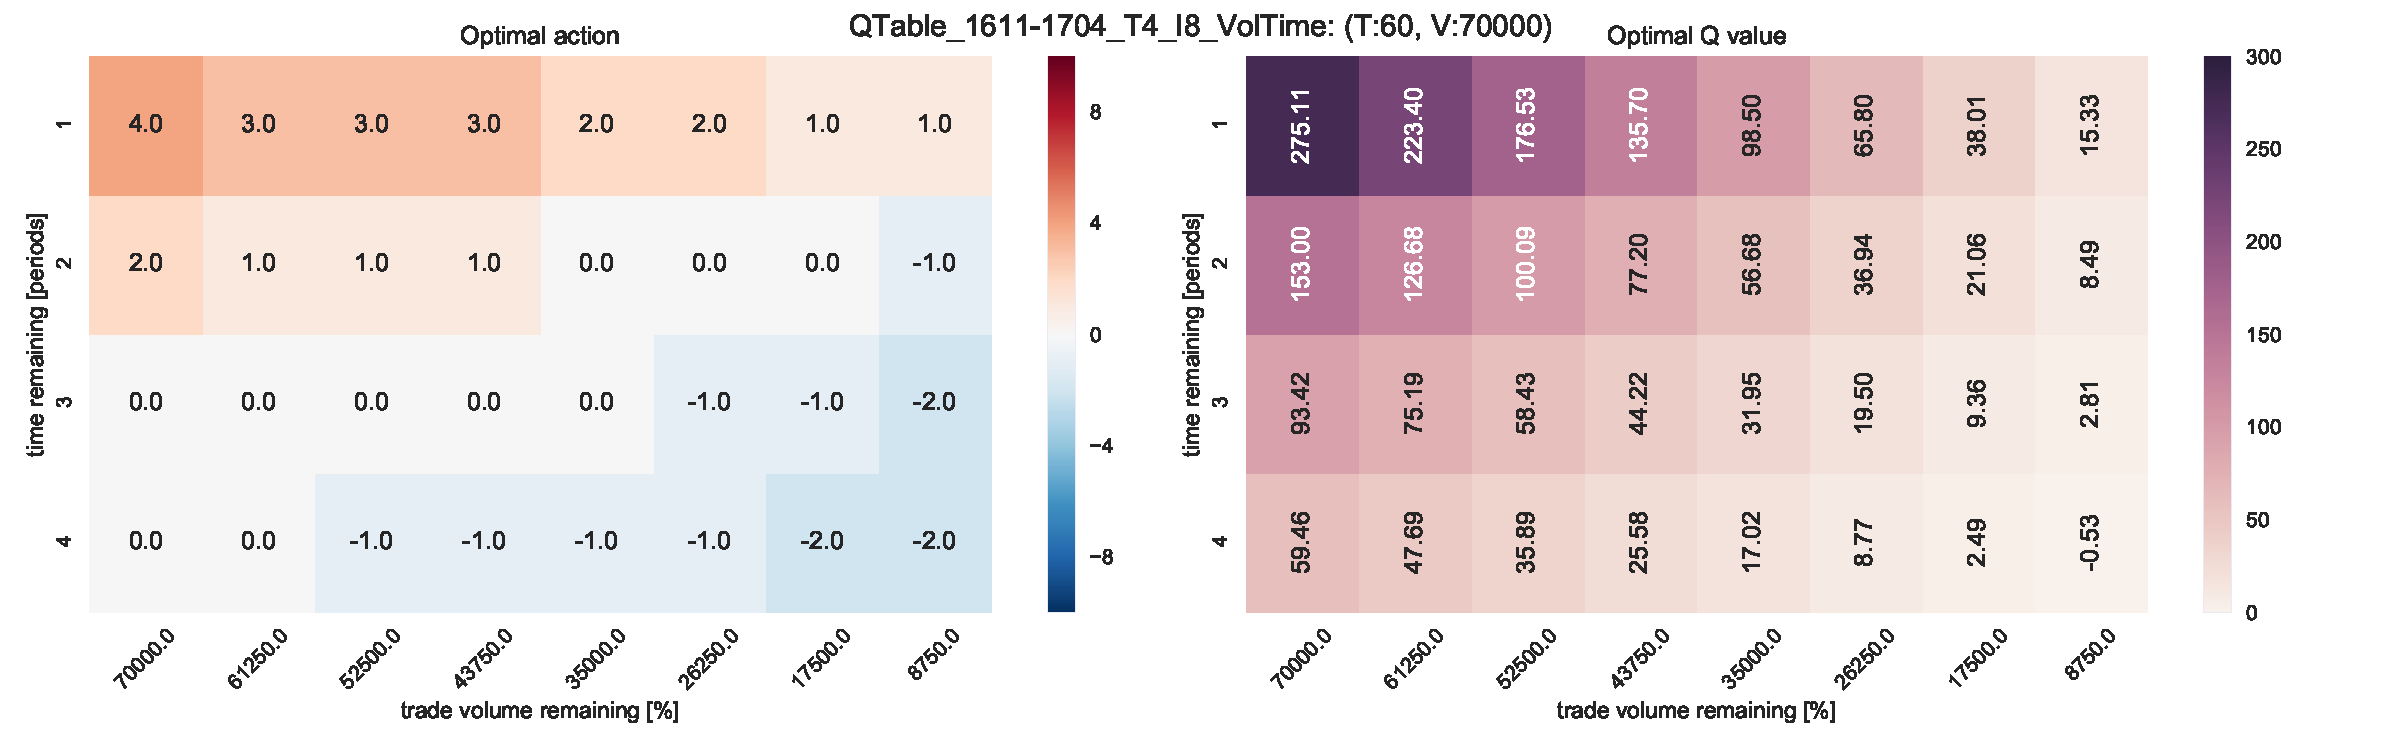
\includegraphics[width=\textwidth]{content/drawings/heatmap_VolTime}
        		\caption{QTable of \lstinline!VolTime!-agent.}
    	\end{subfigure}
	\begin{subfigure}[b]{0.8\textwidth}
        		\centering
        		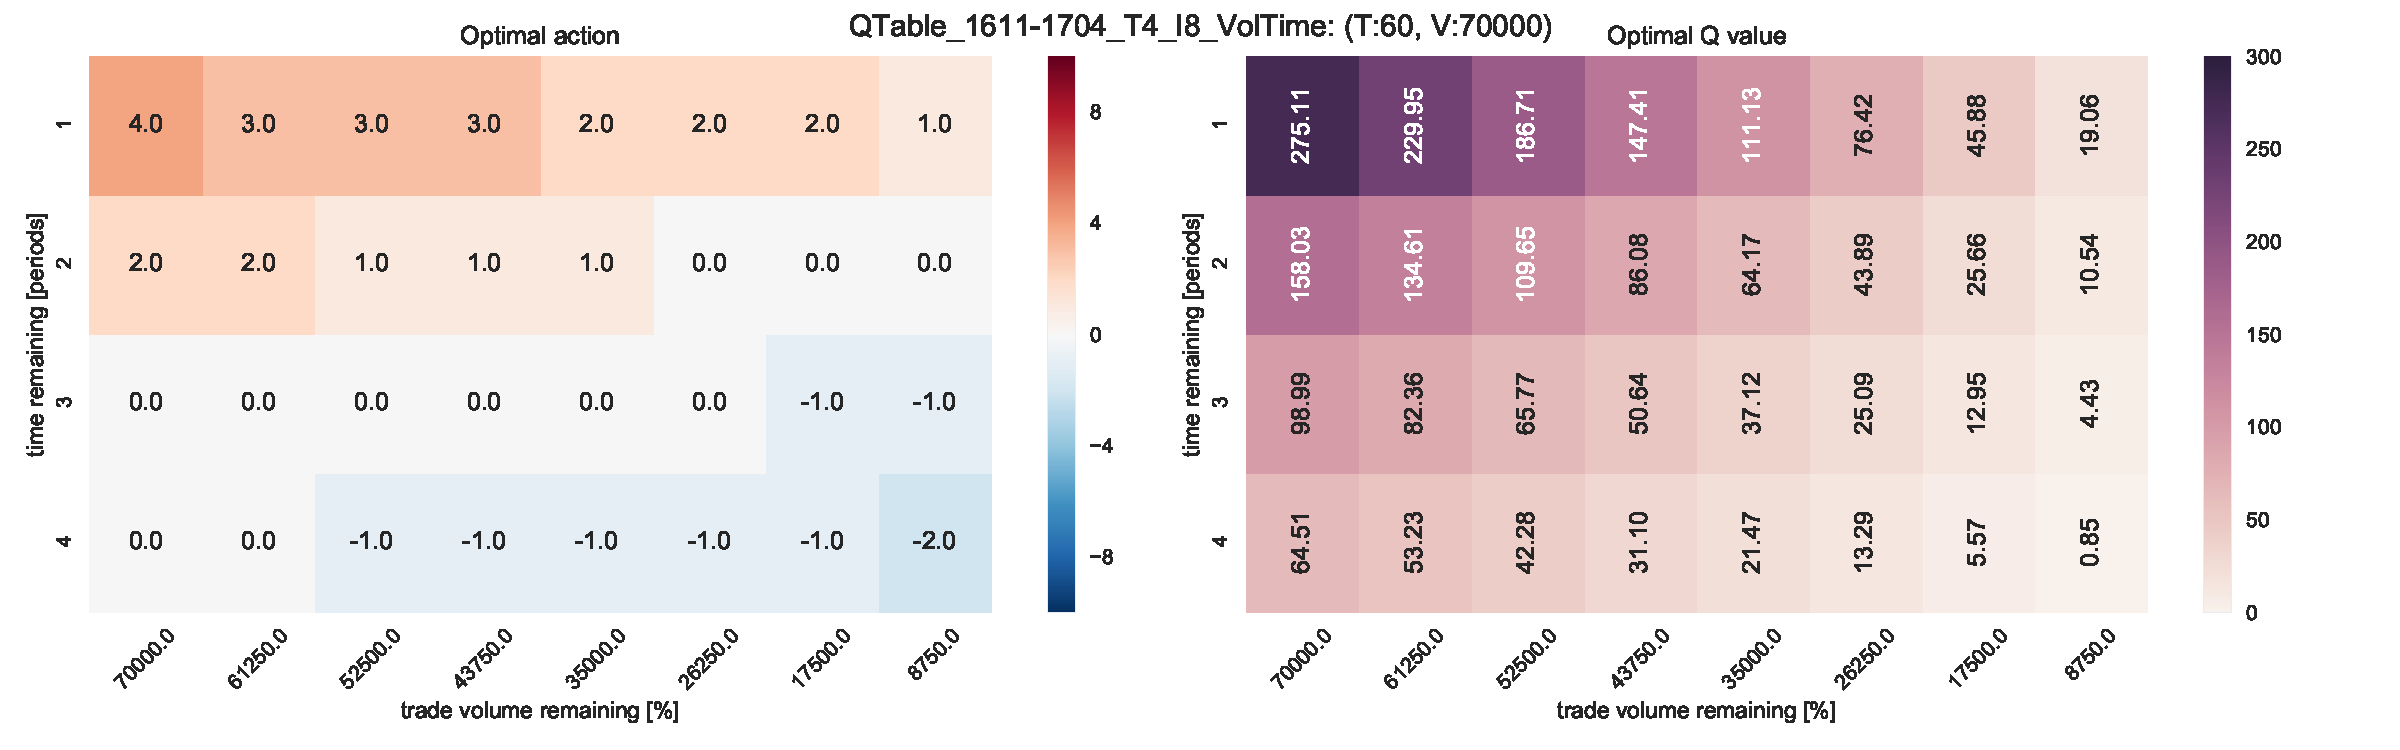
\includegraphics[width=\textwidth]{content/drawings/heatmap_VolTimeSimpre}
        		\caption{QTable of \lstinline!VolTime_simulatedTrades!-agent.}
		
    	\end{subfigure}
	
	\caption{A slight increase in aggression, if preceding trades are incorporated.}
	\label{fig:heatmap:VolTimeSimpre}
	$T=4$, $I=8$, L=15

\end{figure}

The best performing \lstinline!VolTimeSpread_disc5!-agent now undercuts costs induced by simple market orders by $-49.59\%$ (before: $-49.16\%$), the gain in comparison to the optimal \ac{SL} strategy enlarged to $-9.70\%$ (before: $-8.93\%$).\\

\subsection{Estimating Action Effects}
\label{chap:eval:additionalMarketVariables:actioneffects}

\Cref{tab:eval:additionalMarketVariables:_a_} evaluates the impact of adding (lower bound) knowledge about consequences of individual actions to the state space. That way, \lstinline!_a_4_! quotes the minimum volume immediately obtainable by a limit order placed $+0.4\%$ above the current ask price.\\

Potentially due to coarse discretization, these variables cause no major impact. Almost all \lstinline!_a*_!-agents perform worse than the underlying \lstinline!VolTime_simulatedTrades!-agent.

\begin{table}[ht]
	\centering
	\scalebox{0.6}{
	\rowcolors{1}{}{black!5}
\begin{tabular}{|lRRR|RRRR|}
\toprule
{} &  \text{slippage} &     \text{med} &     \text{std} &   \text{perf\_2} &   \text{perf\_4} &   \text{perf\_M} & \text{perf\_VolTime} \\
\midrule
\_a\_-4\_disc5 &    149.84 &   40.54 &  368.50 &  -3.27\% &  -15.04\% &  -46.00\% &       -0.52\% \\
\_a\_-3\_disc5 &    150.70 &   37.95 &  372.15 &  -2.71\% &  -14.55\% &  -45.69\% &        +0.05\% \\
\_a\_0\_disc5  &    153.01 &   45.17 &  375.98 &  -1.22\% &  -13.25\% &  -44.86\% &        +1.58\% \\
\_a\_1\_disc5  &    148.56 &   41.60 &  385.79 &  -4.10\% &  -15.77\% &  -46.46\% &       -1.37\% \\
\_a\_2\_disc5  &    149.47 &   43.47 &  368.49 &  -3.50\% &  -15.25\% &  -46.13\% &       -0.77\% \\
\_a\_3\_disc5  &    145.04 &   42.42 &  365.27 &  -6.37\% &  -17.76\% &  -47.73\% &       -3.71\% \\
\_a\_4\_disc5  &    155.52 &   40.84 &  373.98 &   +0.40\% &  -11.82\% &  -43.95\% &        +3.25\% \\
\_a\_5\_disc5  &    152.05 &   38.53 &  372.03 &  -1.84\% &  -13.79\% &  -45.21\% &        +0.94\% \\
\_a\_6\_disc5  &    151.80 &   40.39 &  371.41 &  -2.00\% &  -13.93\% &  -45.29\% &        +0.78\% \\
\_a\_7\_disc5  &    148.61 &   40.39 &  363.67 &  -4.06\% &  -15.74\% &  -46.44\% &       -1.34\% \\
\_a\_8\_disc5  &    152.46 &   41.26 &  363.02 &  -1.57\% &  -13.56\% &  -45.06\% &        +1.22\% \\
\_a\_9\_disc5  &    151.59 &   40.84 &  363.68 &  -2.14\% &  -14.05\% &  -45.37\% &        +0.64\% \\
\_a\_10\_disc5 &    150.28 &   40.84 &  363.70 &  -2.99\% &  -14.80\% &  -45.84\% &       -0.23\% \\
\midrule
VolTime\_simulatedTrades &    147.86 &   42.10 &  346.17 &   -4.55\% &  -16.17\% &  -46.72\% &       -1.84\% \\
VolTime     &    150.63 &   33.83 &  358.66 &  -2.76\% &  -14.60\% &  -45.72\% &        0.00\% \\
2           &    154.90 &   68.62 &  389.15 &   0.00\% &  -12.17\% &  -44.18\% &        +2.84\% \\
4           &    176.37 &  141.66 &  273.58 &  +13.86\% &    0.00\% &  -36.44\% &       +17.09\% \\
MarketOrder &    277.49 &  246.48 &  158.66 &  +79.14\% &   +57.33\% &    0.00\% &       +84.22\% \\
\bottomrule
\end{tabular}
}  		 
        		\caption{Evaluating the impact of action-consequence knowledge.}
		\small Average performance over the test period may 2017, currency pair USDT/BTC.\\
		
		\label{tab:eval:additionalMarketVariables:_a_}
\end{table}



\subsection{Function Approximation: BatchTree}
\label{chap:experiment:functionApprox}
In a final experiment the look-up table is replaced by an approximation thereof. This eliminates any need for discretization, avoids the cost scaling problem and as such, potentially helps to exploit the underlying sample transitions better. Various \ac{BT}-Agents are trained on the sample transitions collected by the improved backward exploration algorithm, that incorporates preceding trades (see \Cref{chap:exp:simulatedTrades}). Results are shown in \Cref{tab:eval:BatchTree:simPreTrades}.\\

\begin{table}[ht]
	\centering
	\scalebox{0.6}{
\rowcolors{1}{}{black!5}
\begin{tabular}{|lRRR|RRRR|}
\toprule
{} &  \text{slippage} &     \text{med} &     \text{std} &   \text{perf\_2} &   \text{perf\_4} &   \text{perf\_M} & \text{perf\_VolTime} \\
\midrule
BT\_VolTime\_a4\_   &    163.21 &   25.48 &  466.45 &   +5.36\% &   -7.46\% &  -41.18\% &        +8.35\% \\
\cellcolor{green!25}BT\_VolTime\_a*\_       &    \cellcolor{green!25}143.24 &   38.53 &  373.35 &  \cellcolor{green!25}-7.53\% &  -18.78\% &  -48.38\% &       -4.90\% \\
BT\_VolTime &    151.08 &   47.39 &  391.02 &  \cellcolor{black!20}-2.47\% &  -14.34\% &  -45.55\% &        +0.30\% \\
\cellcolor{red!25}BT\_VolTimeSpread &    \cellcolor{red!25}249.07 &  237.29 &  142.11 & \cellcolor{red!25}+60.79\% &   +41.22\% &  -10.24\% &       +65.36\% \\
\midrule
VolTime\_simulatedTrades &    147.86 &   42.10 &  346.17 &   \cellcolor{black!20}-4.55\% &  -16.17\% &  -46.72\% &       -1.84\% \\
VolTime          &    150.63 &   33.83 &  358.66 &  -2.76\% &  -14.60\% &  -45.72\% &        0.00\% \\
2                &    154.90 &   68.62 &  389.15 &   0.00\% &  -12.17\% &  -44.18\% &        +2.84\% \\
4                &    176.37 &  141.66 &  273.58 &  +13.86\% &    0.00\% &  -36.44\% &       +17.09\% \\
MarketOrder      &    277.49 &  246.48 &  158.66 &  +79.14\% &   +57.33\% &    0.00\% &       +84.22\% \\
\bottomrule
\end{tabular}
}  		 
        		\caption{Evaluating the performance of function approximators.}
		\small Average performance over the test period may 2017, currency pair USDT/BTC.\\
		
		\label{tab:eval:BatchTree:simPreTrades}
\end{table}

While the plain \lstinline!BT_VolTime!-agent performs de facto worse than the original, discrete \lstinline!VolTime!-agent ($-2.47\%$ vs. $-4.55\%$),  agents employing individual market variables perform terribly if fed with continuous values. The worst of all, \lstinline!BT_VolTimeSpread!-agent,  performs $+60.79\%$ worse than the optimal \ac{SL} strategy!\\

Conversely, a \ac{BT}-agent trained on all fifteen \lstinline!_a*_effects!-variables simultaneously lifts the \ac{BT} performance from $-2.47\%$ to $-7.53\%$, which is a good result. Unfortunately, it does not catch up with the previously attained $-9.7\%$ (see \Cref{chap:exp:simulatedTrades}).\\


\Cref{fig:heatmap:BatchTree:SimPreTrades} shows exemplary for the plain \lstinline!VolTime!-agent, how the \ac{BT}-agent is able to deliver a more accurate resolution of q-values and optimal actions.

\begin{figure}[ht]
	\centering	
	\begin{subfigure}[b]{0.8\textwidth}
        		\centering
        		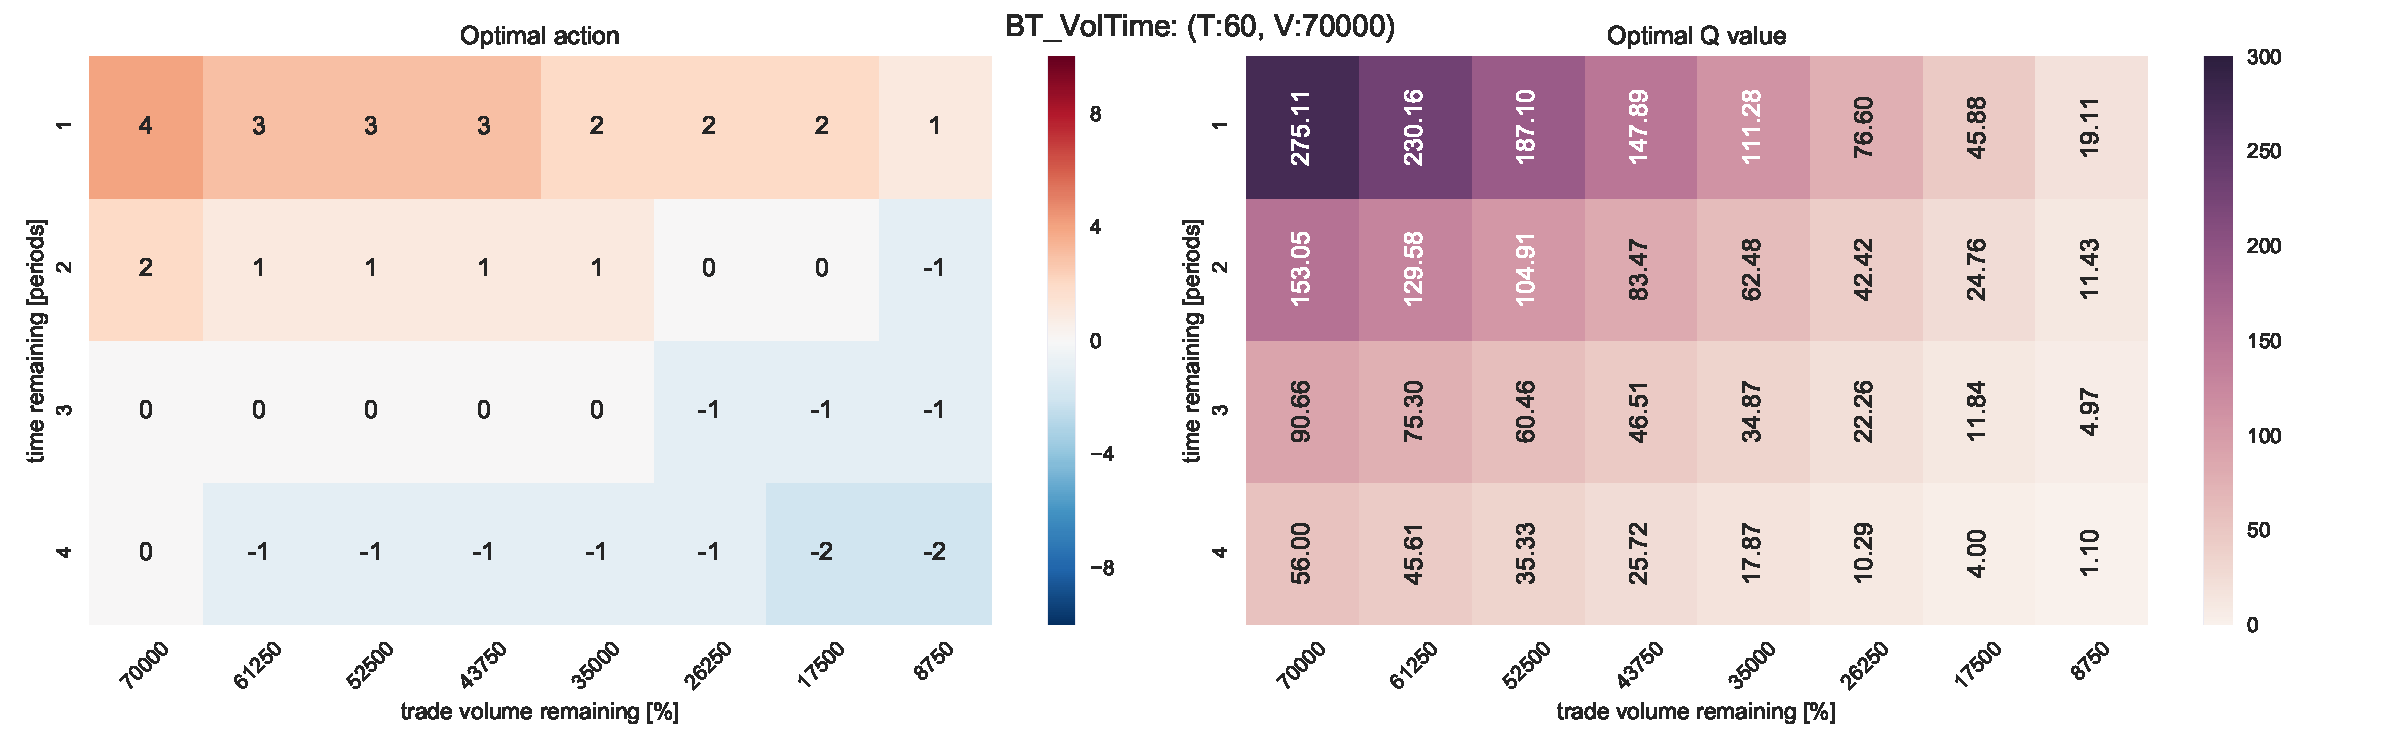
\includegraphics[width=\textwidth]{content/drawings/BT_VolTime_3_vol08}
        		\caption{QTable by \lstinline!VolTime!-agent.}
    	\end{subfigure}
	\begin{subfigure}[b]{0.8\textwidth}
        		\centering
        		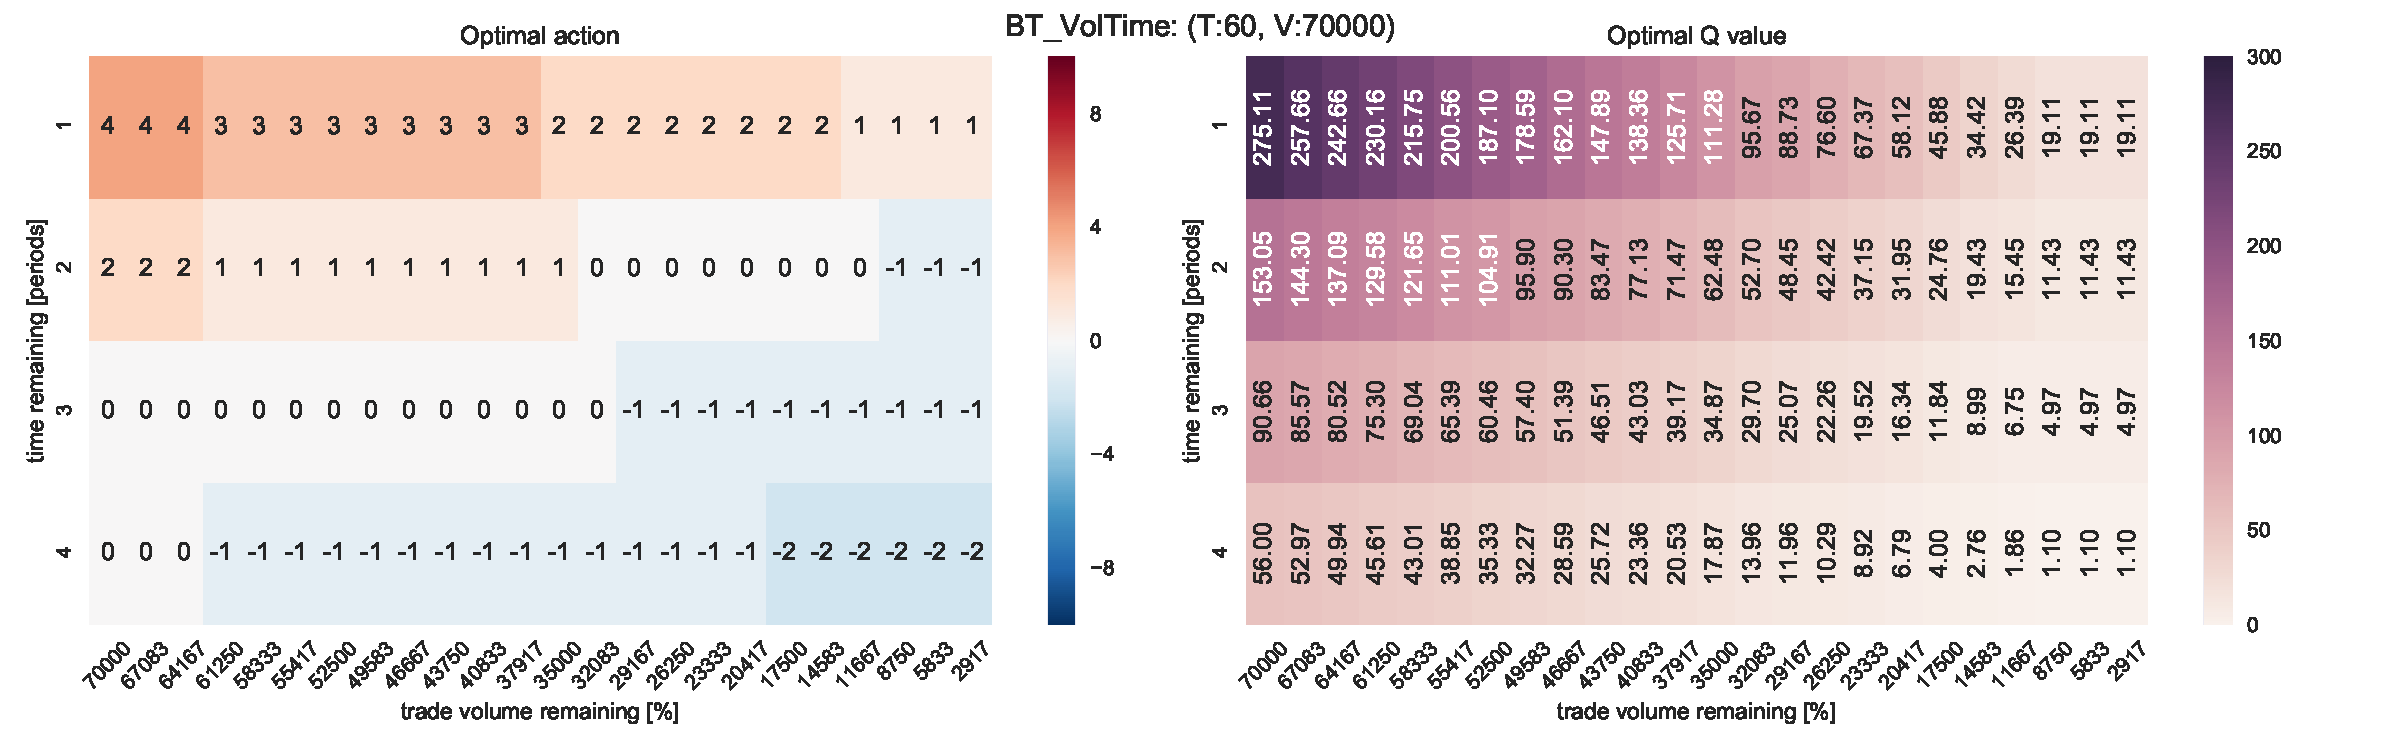
\includegraphics[width=\textwidth]{content/drawings/BT_VolTime_3_vol24}
        		\caption{QTable approximation by \lstinline!BT_VolTime!-agent (High resolution).}
		
    	\end{subfigure}
	
	\caption{The \ac{BT}-agent generalizes to continuous states.}
	\label{fig:heatmap:BatchTree:SimPreTrades}

\end{figure}









\section{Forward Learning}
\label{chap:experiments:forward}
Based on the same training data and simulator settings as used in the preceding Backward Learning Experiments, the novel forward sampling approach, described in \Cref{chap:forwardlearning}, is examined.\\

The \lstinline!BT_Forward!-agent samples from the previously shuffled training data, following an $\epsilon$-greedy strategy. In each exploration phase the respective orderbook window is run through up to 60 times, while only disparate paths are traced. After every 256 exploration phases, the underlying RandomForestRegressor is retrained from scratch, using all transition samples collected to this point. Intermediate models are stored, to document the learning progress over time. The continuous state space consists of both private variables and the fifteen action-effect-variables \lstinline!_a*_!, as introduced in \Cref{chap:exp:additionalmarketvars}.\\

The performance of all sixteen intermediate models is shown in \Cref{tab:eval:ForwardSampling:BT}. Starting vaguely halfway through the training data, the \lstinline!BT_Forward!-agent outperforms all previously examined agents, before the final model constitutes the overall winner with an improvement of $-11.41\%$ over the optimal \ac{SL} strategy.\\

\begin{table}[h!]
	\centering
	\scalebox{0.6}{
\rowcolors{1}{}{black!5}
\begin{tabular}{|lRRR|RRRR|}
\toprule
{} &  \text{slippage} &     \text{med} &     \text{std} &   \text{perf\_2} &   \text{perf\_4} &   \text{perf\_M} & \text{perf\_VolTime} \\
\midrule
BT\_Forward\_samples\_025.078  &    143.72 &   74.69 &  300.93 &   -7.22\% &  -18.52\% &  -48.21\% &       -4.59\% \\
BT\_Forward\_samples\_043.334  &    147.92 &   82.24 &  310.49 &   -4.51\% &  -16.13\% &  -46.69\% &       -1.80\% \\
BT\_Forward\_samples\_061.103  &    149.56 &   77.33 &  288.56 &   -3.45\% &  -15.20\% &  -46.10\% &       -0.71\% \\
BT\_Forward\_samples\_079.809  &    146.67 &   77.20 &  277.43 &   -5.31\% &  -16.84\% &  -47.14\% &       -2.62\% \\
BT\_Forward\_samples\_097.615  &    143.45 &   73.18 &  281.71 &   -7.40\% &  -18.67\% &  -48.31\% &       -4.77\% \\
BT\_Forward\_samples\_116.008 &    144.26 &   77.94 &  285.80 &   -6.87\% &  -18.21\% &  -48.01\% &       -4.23\% \\
BT\_Forward\_samples\_134.011 &    138.22 &   73.30 &  269.71 &  -10.77\% &  -21.63\% &  -50.19\% &       -8.24\% \\
BT\_Forward\_samples\_152.352 &    136.90 &   69.59 &  264.95 &  -11.62\% &  -22.38\% &  -50.66\% &       -9.11\% \\
BT\_Forward\_samples\_170.605 &    137.75 &   77.50 &  261.17 &  -11.07\% &  -21.90\% &  -50.36\% &       -8.55\% \\
BT\_Forward\_samples\_188.224 &    137.64 &   73.71 &  253.37 &  -11.14\% &  -21.96\% &  -50.40\% &       -8.62\% \\
BT\_Forward\_samples\_206.409 &    137.10 &   74.22 &  257.54 &  -11.49\% &  -22.27\% &  -50.59\% &       -8.98\% \\
BT\_Forward\_samples\_224.083 &    142.90 &   75.43 &  265.78 &   -7.75\% &  -18.98\% &  -48.50\% &       -5.13\% \\
BT\_Forward\_samples\_242.342 &    129.85 &   74.43 &  239.96 &  -16.17\% &  -26.37\% &  -53.20\% &      -13.79\% \\
BT\_Forward\_samples\_261.018 &    137.98 &   75.69 &  248.07 &  -10.92\% &  -21.77\% &  -50.27\% &       -8.39\% \\
BT\_Forward\_samples\_279.347 &    138.79 &   75.28 &  258.49 &  -10.40\% &  -21.31\% &  -49.98\% &       -7.86\% \\
BT\_Forward\_samples\_298.020 &    \cellcolor{green!25}137.23 &   \cellcolor{green!25}78.71 &  \cellcolor{green!25}242.88 &  \cellcolor{green!25}-11.41\% &  \cellcolor{green!25}-22.19\% &  \cellcolor{green!25}-50.55\% &       \cellcolor{green!25}-8.89\% \\
\midrule
VolTime                        &    150.63 &   33.83 &  358.66 &   -2.76\% &  -14.60\% &  -45.72\% &        0.00\% \\
2                              &    154.90 &   68.62 &  389.15 &    0.00\% &  -12.17\% &  -44.18\% &        +2.84\% \\
4                              &    176.37 &  141.66 &  273.58 &   +13.86\% &    0.00\% &  -36.44\% &       +17.09\% \\
MarketOrder                    &    277.49 &  246.48 &  158.66 &   +79.14\% &   +57.33\% &    0.00\% &       +84.22\% \\
\bottomrule
\end{tabular}
}  		 
        		\caption{Performance growth of the final \lstinline!BT_Forward!-agent.}
		\small Average performance over the test period may 2017, currency pair USDT/BTC.\\
		
		\label{tab:eval:ForwardSampling:BT}
\end{table}

\Cref{fig:BTForward:performance} visualized the \lstinline!BT_Forward!-agents performance evolution over the training phase. The horizontal lines refer to baselines and previously achieved performances.\\

\begin{figure}[h!]
	\centering
	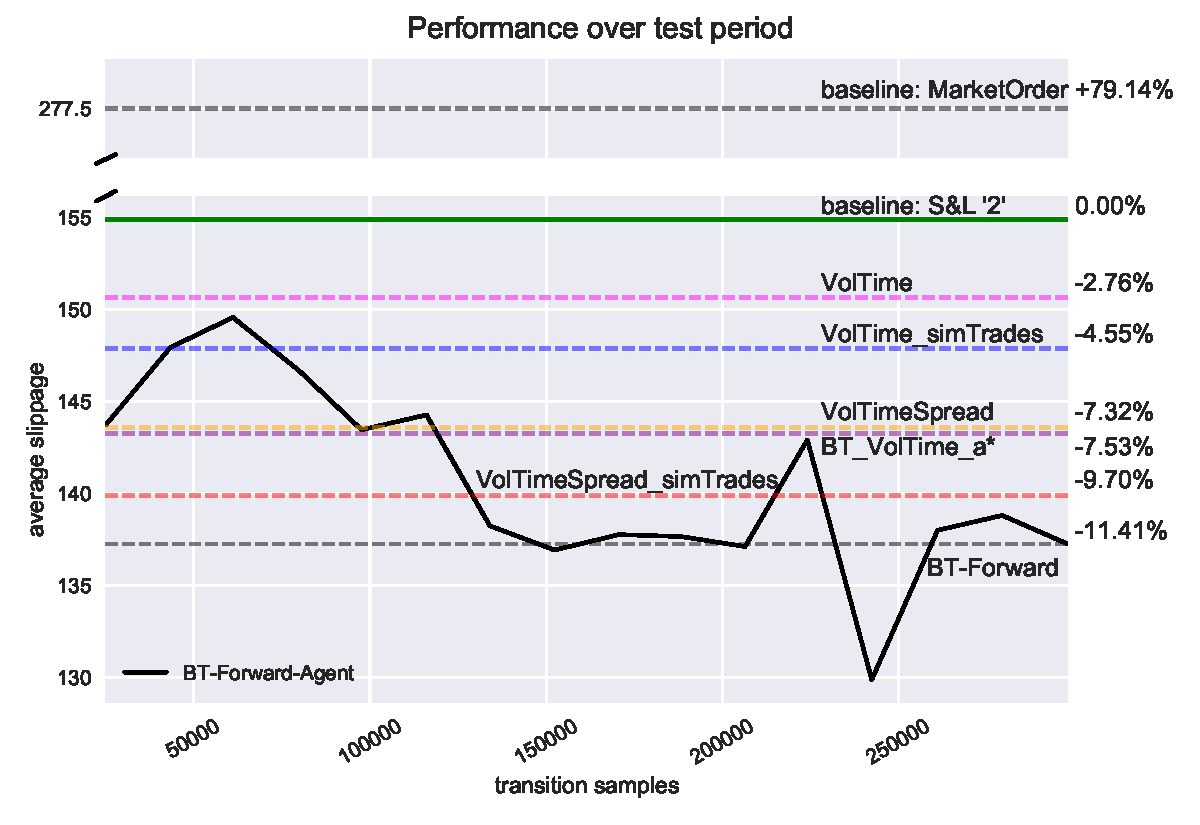
\includegraphics[width=0.8\textwidth]{content/drawings/BT_Forward_Performance}
	\caption{The \lstinline!BT_Forward!-agent performance on the test period.}
	\label{fig:BTForward:performance}

\end{figure}











\cleardoublepage{}
\chapter{Conclusion}\label{chap:conclusion}
Due to the volume of data, the real world example shown in \Cref{chap:example} would have been a tough job on any single local workstation or students notebook. When analyzing big data, it is a great relief or even an inevitable thing to use a cluster of computer for distributed storage and data processing.\\

Hadoop is a great and powerful cluster framework and R is a highly popular and well-advanced programming language for statisticians. In a world of ever growing data, Hadoop and R make a perfect fit. Both combined, the mightful analytic capabilities of R can be applied to big data.




\eject
 

	\appendix
	\pagestyle{scrheadings}
		\settocdepth{section}
			\chapter{Appendix}

\section{Additional Market Variables}
\label{appendix:additionalMarketVariables}
\begin{table}[ht]
	\centering

\scalebox{0.6}{
\begin{tabular}{lRRR|RRRR}
\toprule
{} &  \text{slippage} &     \text{med} &     \text{std} &   \text{perf\_2} &   \text{perf\_4} &   \text{perf\_M} & \text{perf\_VolTime} \\
\midrule
center\_orig\_disc3            &    149.57 &   46.15 &  420.14 &   -3.44\% &  -15.19\% &  -46.10\% &       -0.70\% \\
center\_orig\_disc5            &    161.70 &   37.83 &  450.36 &    +4.39\% &   -8.32\% &  -41.73\% &        +7.35\% \\
center\_orig\_disc9            &    161.65 &   38.83 &  450.40 &    +4.36\% &   -8.35\% &  -41.74\% &        +7.32\% \\
ImmCost\_buy\_worst\_disc3  &    148.35 &   41.26 &  361.17 &   -4.23\% &  -15.89\% &  -46.54\% &       -1.51\% \\
ImmCost\_buy\_worst\_disc5  &    146.83 &   39.62 &  351.77 &   -5.21\% &  -16.75\% &  -47.08\% &       -2.52\% \\
ImmCost\_buy\_worst\_disc9  &    150.53 &   39.66 &  368.95 &   -2.82\% &  -14.65\% &  -45.75\% &       -0.07\% \\
ImmCost\_sell\_worst\_disc3 &    146.72 &   41.91 &  385.13 &   -5.28\% &  -16.81\% &  -47.13\% &       -2.59\% \\
ImmCost\_sell\_worst\_disc5 &    148.94 &   42.71 &  388.86 &   -3.85\% &  -15.55\% &  -46.33\% &       -1.12\% \\
ImmCost\_sell\_worst\_disc9 &    149.28 &   45.05 &  390.19 &   -3.63\% &  -15.36\% &  -46.20\% &       -0.89\% \\
ImmCost\_spread\_disc3     &    150.27 &   40.95 &  355.46 &   -2.99\% &  -14.80\% &  -45.84\% &       -0.23\% \\
ImmCost\_spread\_disc5     &    150.46 &   44.15 &  371.32 &   -2.87\% &  -14.69\% &  -45.78\% &       -0.11\% \\
ImmCost\_spread\_disc9     &    151.98 &   47.12 &  372.53 &   -1.89\% &  -13.83\% &  -45.23\% &        +0.90\% \\
ImmCost\_imbalance\_disc3      &    148.42 &   50.44 &  358.49 &   -4.19\% &  -15.85\% &  -46.51\% &       -1.47\% \\
ImmCost\_imbalance\_disc5      &    150.10 &   68.68 &  336.60 &   -3.10\% &  -14.90\% &  -45.91\% &       -0.35\% \\
ImmCost\_imbalance\_disc9      &    150.50 &   64.44 &  357.22 &   -2.84\% &  -14.67\% &  -45.76\% &       -0.09\% \\
sharecount\_buy\_disc3         &    149.57 &   46.15 &  420.14 &   -3.44\% &  -15.19\% &  -46.10\% &       -0.70\% \\
sharecount\_buy\_disc5         &    160.73 &   37.78 &  449.22 &    +3.76\% &   -8.87\% &  -42.08\% &        +6.70\% \\
sharecount\_buy\_disc9         &    161.65 &   38.83 &  450.40 &    +4.36\% &   -8.35\% &  -41.74\% &        +7.32\% \\
sharecount\_imbalance\_disc3   &    148.57 &   40.68 &  353.91 &   -4.08\% &  -15.76\% &  -46.46\% &       -1.36\% \\
sharecount\_imbalance\_disc5   &    148.03 &   40.49 &  372.86 &   -4.44\% &  -16.07\% &  -46.65\% &       -1.73\% \\
sharecount\_imbalance\_disc9   &    153.27 &   47.28 &  380.38 &   -1.05\% &  -13.10\% &  -44.77\% &        +1.75\% \\
sharecount\_sell\_disc3        &    149.57 &   46.15 &  420.14 &   -3.44\% &  -15.19\% &  -46.10\% &       -0.70\% \\
sharecount\_sell\_disc5        &    151.50 &   47.49 &  425.35 &   -2.20\% &  -14.10\% &  -45.40\% &        +0.58\% \\
sharecount\_sell\_disc9        &    150.37 &   46.15 &  424.22 &   -2.93\% &  -14.75\% &  -45.81\% &       -0.17\% \\
sharecount\_spread\_disc3      &    147.57 &   40.95 &  350.33 &   -4.73\% &  -16.33\% &  -46.82\% &       -2.03\% \\
sharecount\_spread\_disc5      &    148.93 &   40.84 &  352.12 &   -3.86\% &  -15.56\% &  -46.33\% &       -1.13\% \\
sharecount\_spread\_disc9      &    146.61 &   39.62 &  373.00 &   -5.35\% &  -16.87\% &  -47.16\% &       -2.66\% \\
spread\_disc3                 &    147.41 &   35.48 &  370.96 &   -4.84\% &  -16.42\% &  -46.88\% &       -2.14\% \\
spread\_disc5                 &    141.07 &   37.39 &  349.72 &   -8.93\% &  -20.02\% &  -49.16\% &       -6.34\% \\
spread\_disc9                 &    142.80 &   36.69 &  364.76 &   -7.81\% &  -19.03\% &  -48.54\% &       -5.20\% \\
\midrule
ob\_direction\_disc3           &     65.80 &   81.55 &  335.76 &  -57.52\% &  -62.69\% &  -76.29\% &      -56.32\% \\
ob\_direction\_disc5           &     61.99 &   97.52 &  319.84 &  -59.98\% &  -64.85\% &  -77.66\% &      -58.84\% \\
ob\_direction\_disc9           &     57.20 &   86.64 &  321.42 &  -63.07\% &  -67.57\% &  -79.38\% &      -62.02\% \\
future\_center5\_disc3         &    133.58 &   40.40 &  377.88 &  -13.76\% &  -24.26\% &  -51.86\% &      -11.31\% \\
future\_center5\_disc5         &    141.61 &   41.79 &  389.58 &   -8.58\% &  -19.71\% &  -48.97\% &       -5.98\% \\
future\_center15\_disc3        &    107.74 &   31.91 &  364.92 &  -30.44\% &  -38.91\% &  -61.17\% &      -28.47\% \\
future\_center15\_disc5        &    133.78 &   40.90 &  405.88 &  -13.63\% &  -24.15\% &  -51.79\% &      -11.18\% \\
future\_center15\_disc9        &    121.11 &   47.41 &  411.10 &  -21.82\% &  -31.33\% &  -56.36\% &      -19.60\% \\
future\_center60\_disc3        &    139.20 &   36.02 &  398.05 &  -10.14\% &  -21.07\% &  -49.83\% &       -7.58\% \\
future\_center60\_disc5        &    131.85 &   47.63 &  391.46 &  -14.88\% &  -25.25\% &  -52.49\% &      -12.47\% \\
future\_center60\_disc9        &    131.57 &   48.52 &  422.35 &  -15.06\% &  -25.40\% &  -52.59\% &      -12.65\% \\
\midrule
VolTime                      &    150.63 &   33.83 &  358.66 &   -2.76\% &  -14.60\% &  -45.72\% &        0.00\% \\
2                            &    154.90 &   68.62 &  389.15 &    0.00\% &  -12.17\% &  -44.18\% &        +2.84\% \\
4                            &    176.37 &  141.66 &  273.58 &   +13.86\% &    0.00\% &  -36.44\% &       +17.09\% \\
MarketOrder                  &    277.49 &  246.48 &  158.66 &   +79.14\% &   +57.33\% &    0.00\% &       +84.22\% \\
\bottomrule
\end{tabular}
}

        		\caption[Full version of \Cref{tab:eval:additionalMarketVariables}]{Average trading costs within the test period May 2017.}
		See \Cref{chap:exp:additionalmarketvars} for the actual experiment description. This is the full version of \Cref{tab:eval:additionalMarketVariables}.
		\label{tab:eval:additionalMarketVariables:fulltable}

\end{table}




\section{Constant Market Variables}
\label{appendix:fixedMarketVars}
\begin{table}[ht]
	\centering

\scalebox{0.6}{
\begin{tabular}{lRRR|RRRR}
\toprule
{} &  \text{slippage} &     \text{med} &     \text{std} &   \text{perf\_2} &   \text{perf\_4} &   \text{perf\_M} & \text{perf\_VolTime} \\
\midrule
VolTime                      &    150.63 &   33.83 &  358.66 &   95.04\% &   85.40\% &   54.28\% &      100.00\% \\
center\_orig\_disc3            &    149.57 &   46.15 &  420.14 &   94.37\% &   84.81\% &   53.90\% &       99.30\% \\
center\_orig\_disc5            &    150.37 &   47.01 &  422.14 &   94.88\% &   85.26\% &   54.19\% &       99.83\% \\
center\_orig\_disc9            &    149.76 &   46.15 &  420.67 &   94.49\% &   84.91\% &   53.97\% &       99.43\% \\
ImmCost\_buy\_worst\_disc3  &    149.46 &   44.67 &  398.72 &   94.31\% &   84.74\% &   53.86\% &       99.23\% \\
ImmCost\_buy\_worst\_disc5  &    150.22 &   50.15 &  402.48 &   94.78\% &   85.17\% &   54.13\% &       99.73\% \\
ImmCost\_buy\_worst\_disc9  &    155.55 &   44.67 &  417.02 &   98.14\% &   88.19\% &   56.06\% &      103.27\% \\
ImmCost\_sell\_worst\_disc3 &    150.13 &   41.26 &  352.48 &   94.73\% &   85.12\% &   54.10\% &       99.67\% \\
ImmCost\_sell\_worst\_disc5 &    157.24 &   42.71 &  378.90 &   99.21\% &   89.15\% &   56.67\% &      104.39\% \\
ImmCost\_sell\_worst\_disc9 &    148.66 &   48.86 &  360.92 &   93.80\% &   84.29\% &   53.57\% &       98.69\% \\
ImmCost\_spread\_disc3     &    152.15 &   51.32 &  391.87 &   96.00\% &   86.26\% &   54.83\% &      101.01\% \\
ImmCost\_spread\_disc5     &    151.25 &   53.07 &  397.30 &   95.43\% &   85.75\% &   54.51\% &      100.41\% \\
ImmCost\_spread\_disc9     &    150.43 &   41.60 &  382.41 &   94.91\% &   85.29\% &   54.21\% &       99.87\% \\
ImmCost\_imbalance\_disc3      &    148.05 &   51.06 &  379.25 &   93.41\% &   83.94\% &   53.35\% &       98.29\% \\
ImmCost\_imbalance\_disc5      &    147.26 &   47.03 &  383.23 &   92.91\% &   83.49\% &   53.07\% &       97.76\% \\
ImmCost\_imbalance\_disc9      &    146.76 &   53.75 &  377.13 &   92.60\% &   83.21\% &   52.89\% &       97.43\% \\
sharecount\_buy\_disc3         &    149.57 &   46.15 &  420.14 &   94.37\% &   84.81\% &   53.90\% &       99.30\% \\
sharecount\_buy\_disc5         &    150.37 &   47.01 &  422.14 &   94.88\% &   85.26\% &   54.19\% &       99.83\% \\
sharecount\_buy\_disc9         &    149.76 &   46.15 &  420.67 &   94.49\% &   84.91\% &   53.97\% &       99.43\% \\
sharecount\_imbalance\_disc3   &    151.21 &   52.13 &  397.27 &   95.40\% &   85.73\% &   54.49\% &      100.39\% \\
sharecount\_imbalance\_disc5   &    152.44 &   53.41 &  400.89 &   96.18\% &   86.43\% &   54.94\% &      101.21\% \\
sharecount\_imbalance\_disc9   &    155.03 &   57.56 &  394.20 &   97.81\% &   87.90\% &   55.87\% &      102.92\% \\
sharecount\_sell\_disc3        &    149.57 &   46.15 &  420.14 &   94.37\% &   84.81\% &   53.90\% &       99.30\% \\
sharecount\_sell\_disc5        &    150.37 &   47.01 &  422.14 &   94.88\% &   85.26\% &   54.19\% &       99.83\% \\
sharecount\_sell\_disc9        &    149.53 &   46.15 &  420.50 &   94.35\% &   84.78\% &   53.89\% &       99.27\% \\
sharecount\_spread\_disc3      &    150.66 &   48.23 &  419.32 &   95.06\% &   85.42\% &   54.29\% &      100.02\% \\
sharecount\_spread\_disc5      &    149.23 &   53.41 &  402.65 &   94.16\% &   84.61\% &   53.78\% &       99.07\% \\
sharecount\_spread\_disc9      &    148.64 &   52.13 &  408.67 &   93.78\% &   84.27\% &   53.57\% &       98.68\% \\
spread\_disc3                 &    148.83 &   41.70 &  360.98 &   93.91\% &   84.39\% &   53.64\% &       98.81\% \\
spread\_disc5                 &    143.12 &   40.78 &  350.14 &   90.30\% &   81.15\% &   51.58\% &       95.02\% \\
spread\_disc9                 &    144.66 &   43.25 &  352.39 &   91.27\% &   82.02\% &   52.13\% &       96.04\% \\
2                            &    158.49 &   69.66 &  400.59 &  100.00\% &   89.86\% &   57.12\% &      105.22\% \\
4                            &    176.37 &  141.66 &  273.58 &  111.28\% &  100.00\% &   63.56\% &      117.09\% \\
MarketOrder                  &    277.49 &  246.48 &  158.66 &  175.08\% &  157.33\% &  100.00\% &      184.22\% \\
\bottomrule
\end{tabular}
}

        		\caption[Full version of \Cref{tab:eval:additionalMarketVariables}]{Average trading costs within the test period May 2017.}
		See \Cref{chap:exp:additionalmarketvars:constant} for the actual experiment description. This is the full version of \Cref{tab:eval:additionalMarketVariables:fixed}.
		\label{tab:eval:additionalMarketVariables:fixed:fulltable}
\end{table}





















\section{Simulation of preceding trades}
\label{appendix:simPreTrades}
\begin{table}[ht]
	\centering

\scalebox{0.6}{
\begin{tabular}{lRRR|RRRR}
\toprule
{} &  \text{slippage} &     \text{med} &     \text{std} &   \text{perf\_2} &   \text{perf\_4} &   \text{perf\_M} & \text{perf\_VolTime} \\
\midrule
center\_orig\_disc3              &    158.97 &   48.93 &  431.16 &    +2.62\% &   -9.87\% &  -42.71\% &        +5.54\% \\
center\_orig\_disc5              &    150.47 &   47.49 &  422.12 &   -2.86\% &  -14.69\% &  -45.78\% &       -0.11\% \\
center\_orig\_disc9              &    149.76 &   46.15 &  420.66 &   -3.32\% &  -15.09\% &  -46.03\% &       -0.57\% \\
ImmCost\_buy\_worst\_disc3    &    148.49 &   45.78 &  396.35 &   -4.14\% &  -15.81\% &  -46.49\% &       -1.42\% \\
ImmCost\_buy\_worst\_disc5    &    148.33 &   47.46 &  400.73 &   -4.24\% &  -15.90\% &  -46.55\% &       -1.53\% \\
ImmCost\_buy\_worst\_disc9    &    154.36 &   39.16 &  414.24 &   -0.35\% &  -12.48\% &  -44.37\% &        +2.48\% \\
ImmCost\_sell\_worst\_disc3   &    150.23 &   40.84 &  351.30 &   -3.02\% &  -14.82\% &  -45.86\% &       -0.26\% \\
ImmCost\_sell\_worst\_disc5   &    154.06 &   42.10 &  370.91 &   -0.54\% &  -12.65\% &  -44.48\% &        +2.28\% \\
ImmCost\_sell\_worst\_disc9   &    152.07 &   49.16 &  362.68 &   -1.83\% &  -13.78\% &  -45.20\% &        +0.96\% \\
ImmCost\_spread\_disc3       &    151.10 &   52.13 &  390.08 &   -2.45\% &  -14.33\% &  -45.55\% &        +0.31\% \\
ImmCost\_spread\_disc5       &    151.12 &   53.07 &  395.68 &   -2.44\% &  -14.32\% &  -45.54\% &        +0.33\% \\
ImmCost\_spread\_disc9       &    148.45 &   41.60 &  380.40 &   -4.16\% &  -15.83\% &  -46.50\% &       -1.44\% \\
ImmCost\_imbalance\_disc3        &    145.82 &   47.88 &  374.09 &   -5.86\% &  -17.32\% &  -47.45\% &       -3.19\% \\
ImmCost\_imbalance\_disc5        &    143.86 &   47.05 &  375.43 &   -7.13\% &  -18.44\% &  -48.16\% &       -4.49\% \\
ImmCost\_imbalance\_disc9        &    144.90 &   51.39 &  365.94 &   -6.45\% &  -17.84\% &  -47.78\% &       -3.80\% \\
sharecount\_buy\_disc3           &    149.57 &   46.15 &  420.14 &   -3.44\% &  -15.19\% &  -46.10\% &       -0.70\% \\
sharecount\_buy\_disc5           &    150.47 &   47.49 &  422.12 &   -2.86\% &  -14.69\% &  -45.78\% &       -0.11\% \\
sharecount\_buy\_disc9           &    149.76 &   46.15 &  420.67 &   -3.32\% &  -15.09\% &  -46.03\% &       -0.57\% \\
sharecount\_imbalance\_disc3     &    153.26 &   53.41 &  398.42 &   -1.06\% &  -13.10\% &  -44.77\% &        +1.75\% \\
sharecount\_imbalance\_disc5     &    151.92 &   53.41 &  400.69 &   -1.92\% &  -13.86\% &  -45.25\% &        +0.86\% \\
sharecount\_imbalance\_disc9     &    154.33 &   57.43 &  394.25 &   -0.37\% &  -12.49\% &  -44.38\% &        +2.46\% \\
sharecount\_sell\_disc3          &    149.57 &   46.15 &  420.14 &   -3.44\% &  -15.19\% &  -46.10\% &       -0.70\% \\
sharecount\_sell\_disc5          &    149.93 &   47.01 &  420.70 &   -3.21\% &  -14.99\% &  -45.97\% &       -0.47\% \\
sharecount\_sell\_disc9          &    149.53 &   46.15 &  420.50 &   -3.47\% &  -15.22\% &  -46.11\% &       -0.73\% \\
sharecount\_spread\_disc3        &    150.35 &   48.23 &  418.91 &   -2.94\% &  -14.76\% &  -45.82\% &       -0.19\% \\
sharecount\_spread\_disc5        &    149.36 &   53.41 &  402.86 &   -3.58\% &  -15.31\% &  -46.17\% &       -0.84\% \\
sharecount\_spread\_disc9        &    148.47 &   50.52 &  410.27 &   -4.15\% &  -15.82\% &  -46.50\% &       -1.43\% \\
spread\_disc3                   &    145.63 &   41.89 &  346.00 &   -5.98\% &  -17.43\% &  -47.52\% &       -3.32\% \\
spread\_disc5                   &    139.87 &   41.22 &  336.30 &   -9.70\% &  -20.69\% &  -49.59\% &       -7.14\% \\
spread\_disc9                   &    141.30 &   42.80 &  336.88 &   -8.78\% &  -19.89\% &  -49.08\% &       -6.19\% \\
\midrule
ob\_direction\_disc3             &     69.01 &  101.49 &  323.00 &  -55.45\% &  -60.87\% &  -75.13\% &      -54.18\% \\
ob\_direction\_disc5             &     62.03 &   97.52 &  320.76 &  -59.95\% &  -64.83\% &  -77.64\% &      -58.82\% \\
ob\_direction\_disc9             &     57.74 &   87.92 &  321.20 &  -62.73\% &  -67.26\% &  -79.19\% &      -61.67\% \\
\midrule
VolTime\_simulatedTrades &    147.86 &   42.10 &  346.17 &   -4.55\% &  -16.17\% &  -46.72\% &       -1.84\% \\
VolTime                        &    150.63 &   33.83 &  358.66 &   -2.76\% &  -14.60\% &  -45.72\% &        0.00\% \\
2                              &    154.90 &   68.62 &  389.15 &    0.00\% &  -12.17\% &  -44.18\% &        +2.84\% \\
4                              &    176.37 &  141.66 &  273.58 &   +13.86\% &    0.00\% &  -36.44\% &       +17.09\% \\
MarketOrder                    &    277.49 &  246.48 &  158.66 &   +79.14\% &   +57.33\% &    0.00\% &      +84.22\% \\
\bottomrule
\end{tabular}}

        		\caption[Full version of \Cref{tab:eval:additionalMarketVariables:simulatedTrades}]{Average trading costs within the test period May 2017.}
		See \Cref{chap:exp:simulatedTrades} for the actual experiment description. This is the full version of \Cref{tab:eval:additionalMarketVariables:simulatedTrades}.
		\label{tab:eval:additionalMarketVariables:simulatedTrades:fulltable}
\end{table}
			\clearpage
				 
	\backmatter
		\pagestyle{empty}
			\chapter{Glossary}
				\begin{acronym}
					\acro{OTS}{Orderbook Trading Simulator}
					\acro{RL}{Reinforcement Learning}	
					\acro{SL}[S\&L]{Submit \& Leave Strategy}
					\acro{SR}[S\&R]{Submit \& Revise Strategy}
					\acro{NASDAQ}{National Association of Securities Dealers Automated Quotations (American Stock Exchange))}	
				\end{acronym}
			%\printbibliography[heading=bibintoc]
%\printbibliography[heading=bibnumbered]  
\chapter{References}
\printbibliography[heading=none]  %Überschrift von chapter
%    \adjustmtc % minitoc fix

\eject
%\clearpage
			\listoffigures 

\listoftables 

\lstlistoflistings

\begingroup 
  \let\chapter=\section

    \listofalgorithms
 \endgroup 

			
\end{document}